%%%%%%%%%%%%%%%%%%%%%%%%%%%%%%%%%%%%
\label{sec:gbb-data_mc_comp}

The flavor fraction fits are performed in each bins of each observable to determine the $b\bar b $ fractions in data. 

\subsection{$\Delta R$}

In total, there are six bins of the $\Delta R$ observable we are measuring. The flavor fraction fits are performed in $\Delta R \in\{[0.2, 0.25], [0.25, 0.3], [0.3, 0.4], [0.4,0.5], [0.5,0.6], [0.6,0.7]\}$. The pre-fit and post-fit Data/MC comparison are shown in Figures~\ref{fig:dR-prefits-leading},\ref{fig:dR-prefits-subleading},\ref{fig:dR-postfits-leading},\ref{fig:dR-postfits-subleading}. The MC predicted and fitted fraction of each flavor component are shown in Fig>~\ref{fig:dR-fitfrac}. Four sets of fit cross check are performed: (1) using \sdzero as discriminant (2) using \subsubsdzero (3) using $p_T$ parameterized templates and (4) without track jet kinematic reweighting. The cross check results are summarized in Fig.~\ref{fig:dR-fitfrac-crosscheck}. We observe closure of the fitted signal (`BB') event fraction in all the cross checks within fitting uncertainties. The size of each of the systematic uncertainty is summarized in Table~\ref{tab:dRsys}.

\begin{figure}[htbp]
  \centering
 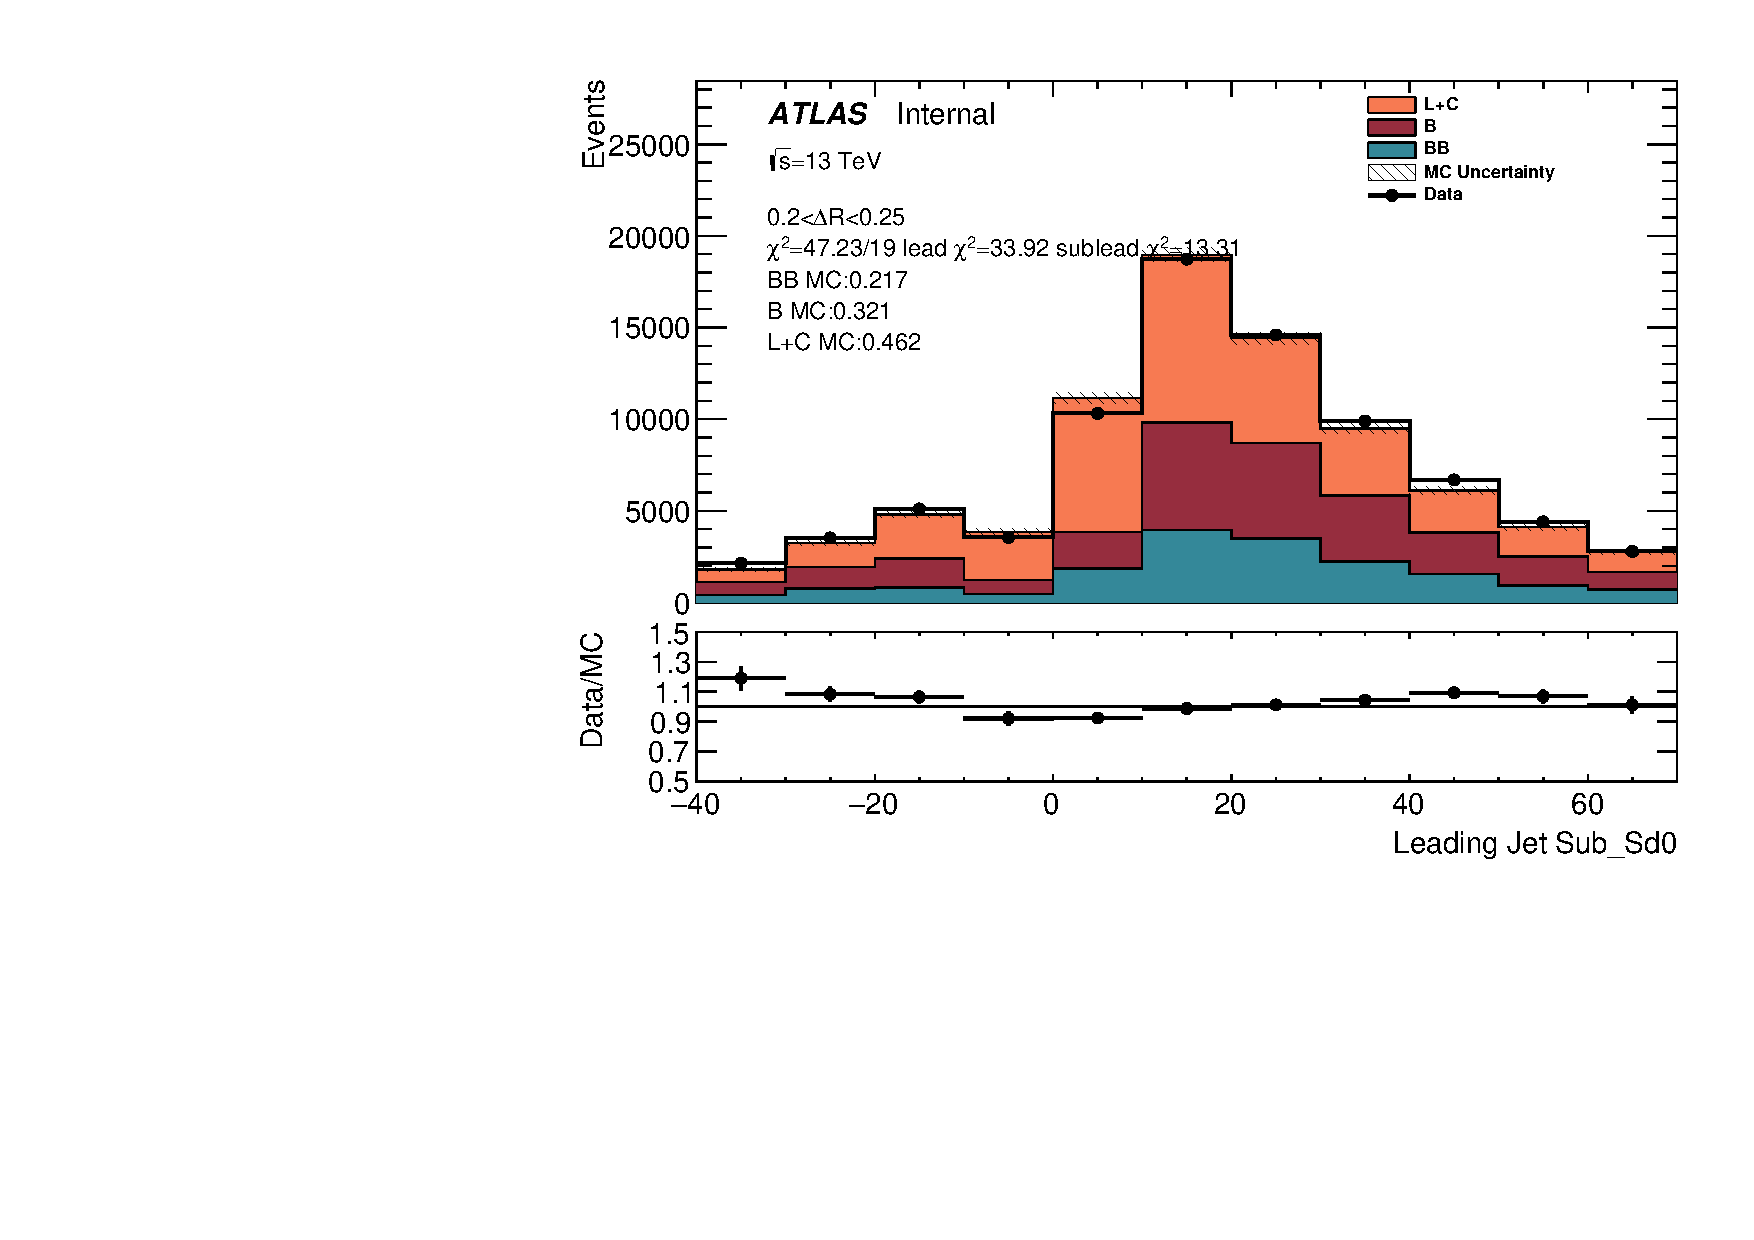
\includegraphics[width=0.32\textwidth]{figures/gbb/Sub_Sd0_Fits/Canv_PreFit_02-DeltaR-025_LpT_INF_SpT_INF_coarse_x.pdf}
 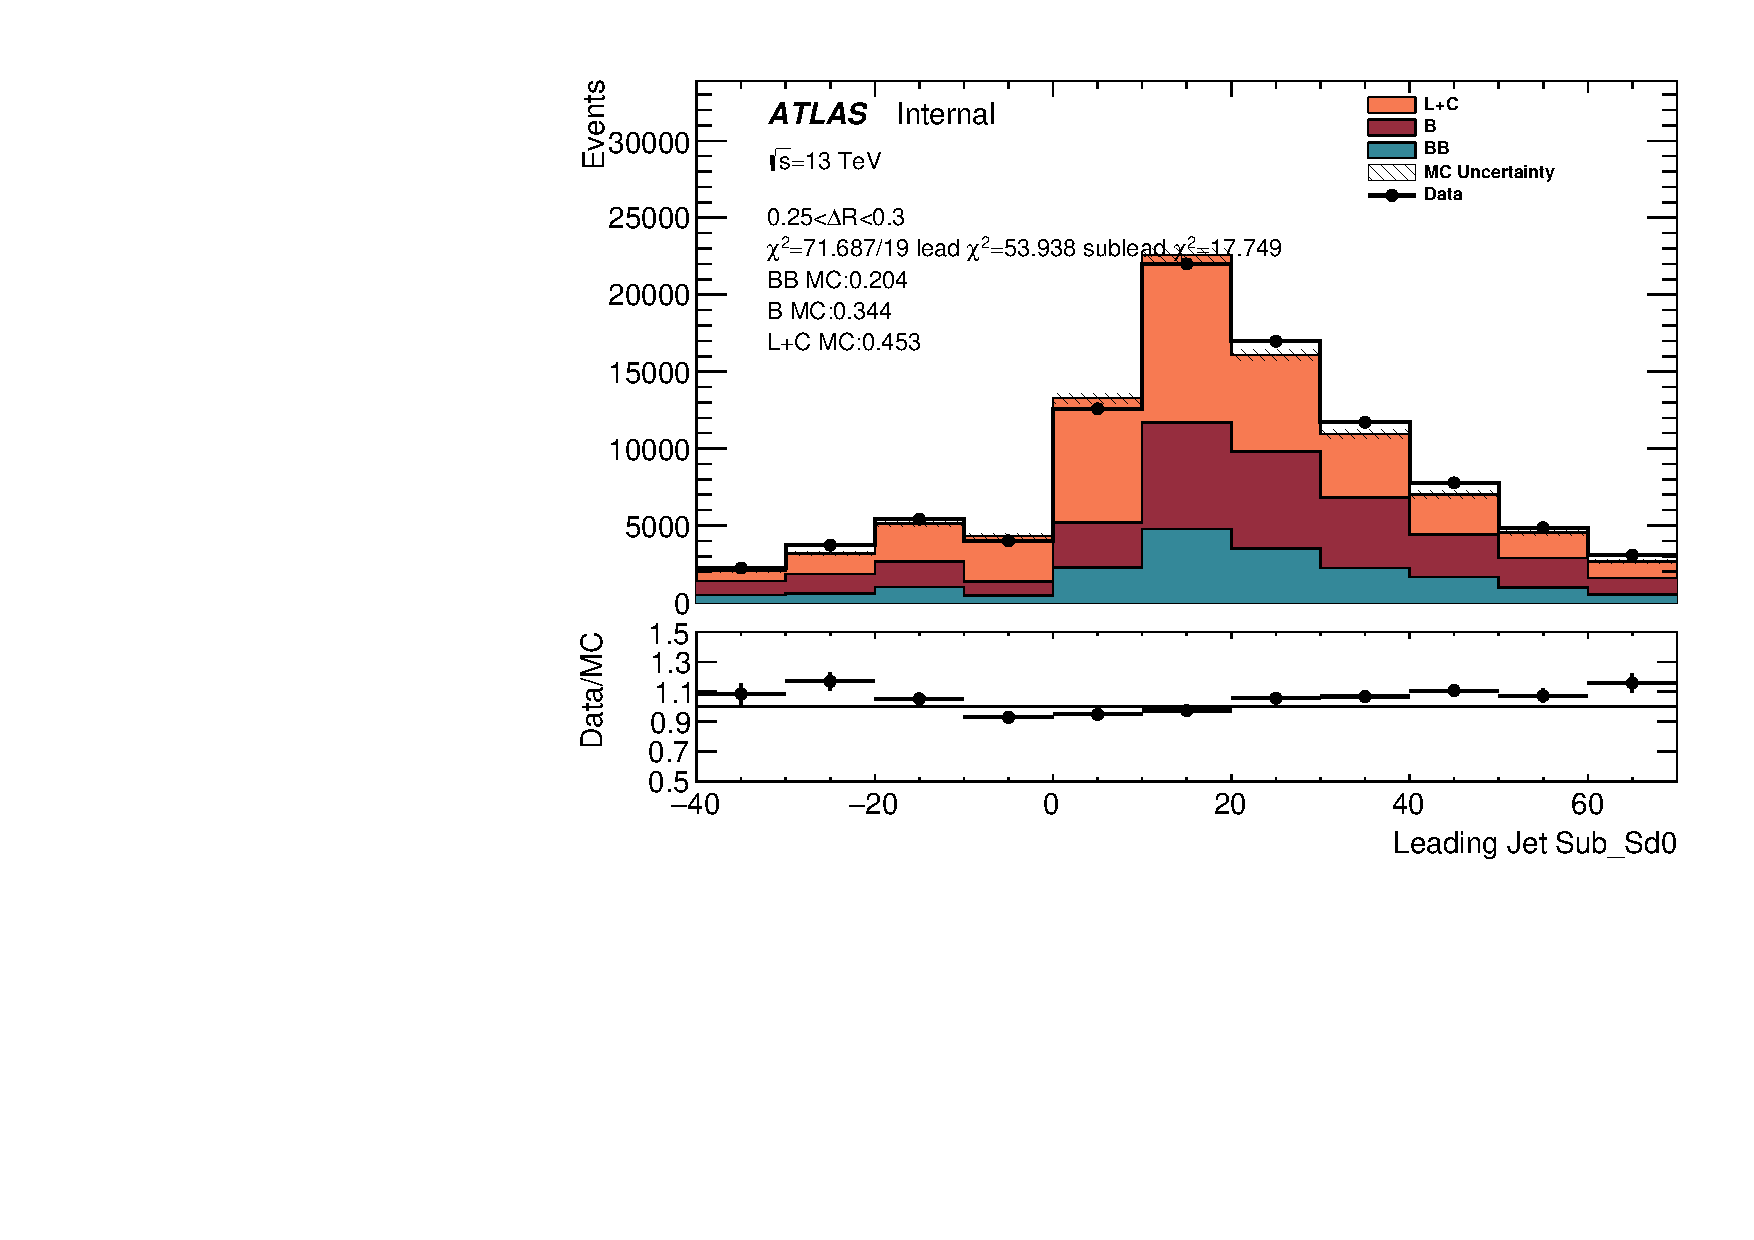
\includegraphics[width=0.32\textwidth]{figures/gbb/Sub_Sd0_Fits/Canv_PreFit_025-DeltaR-03_LpT_INF_SpT_INF_coarse_x.pdf}
 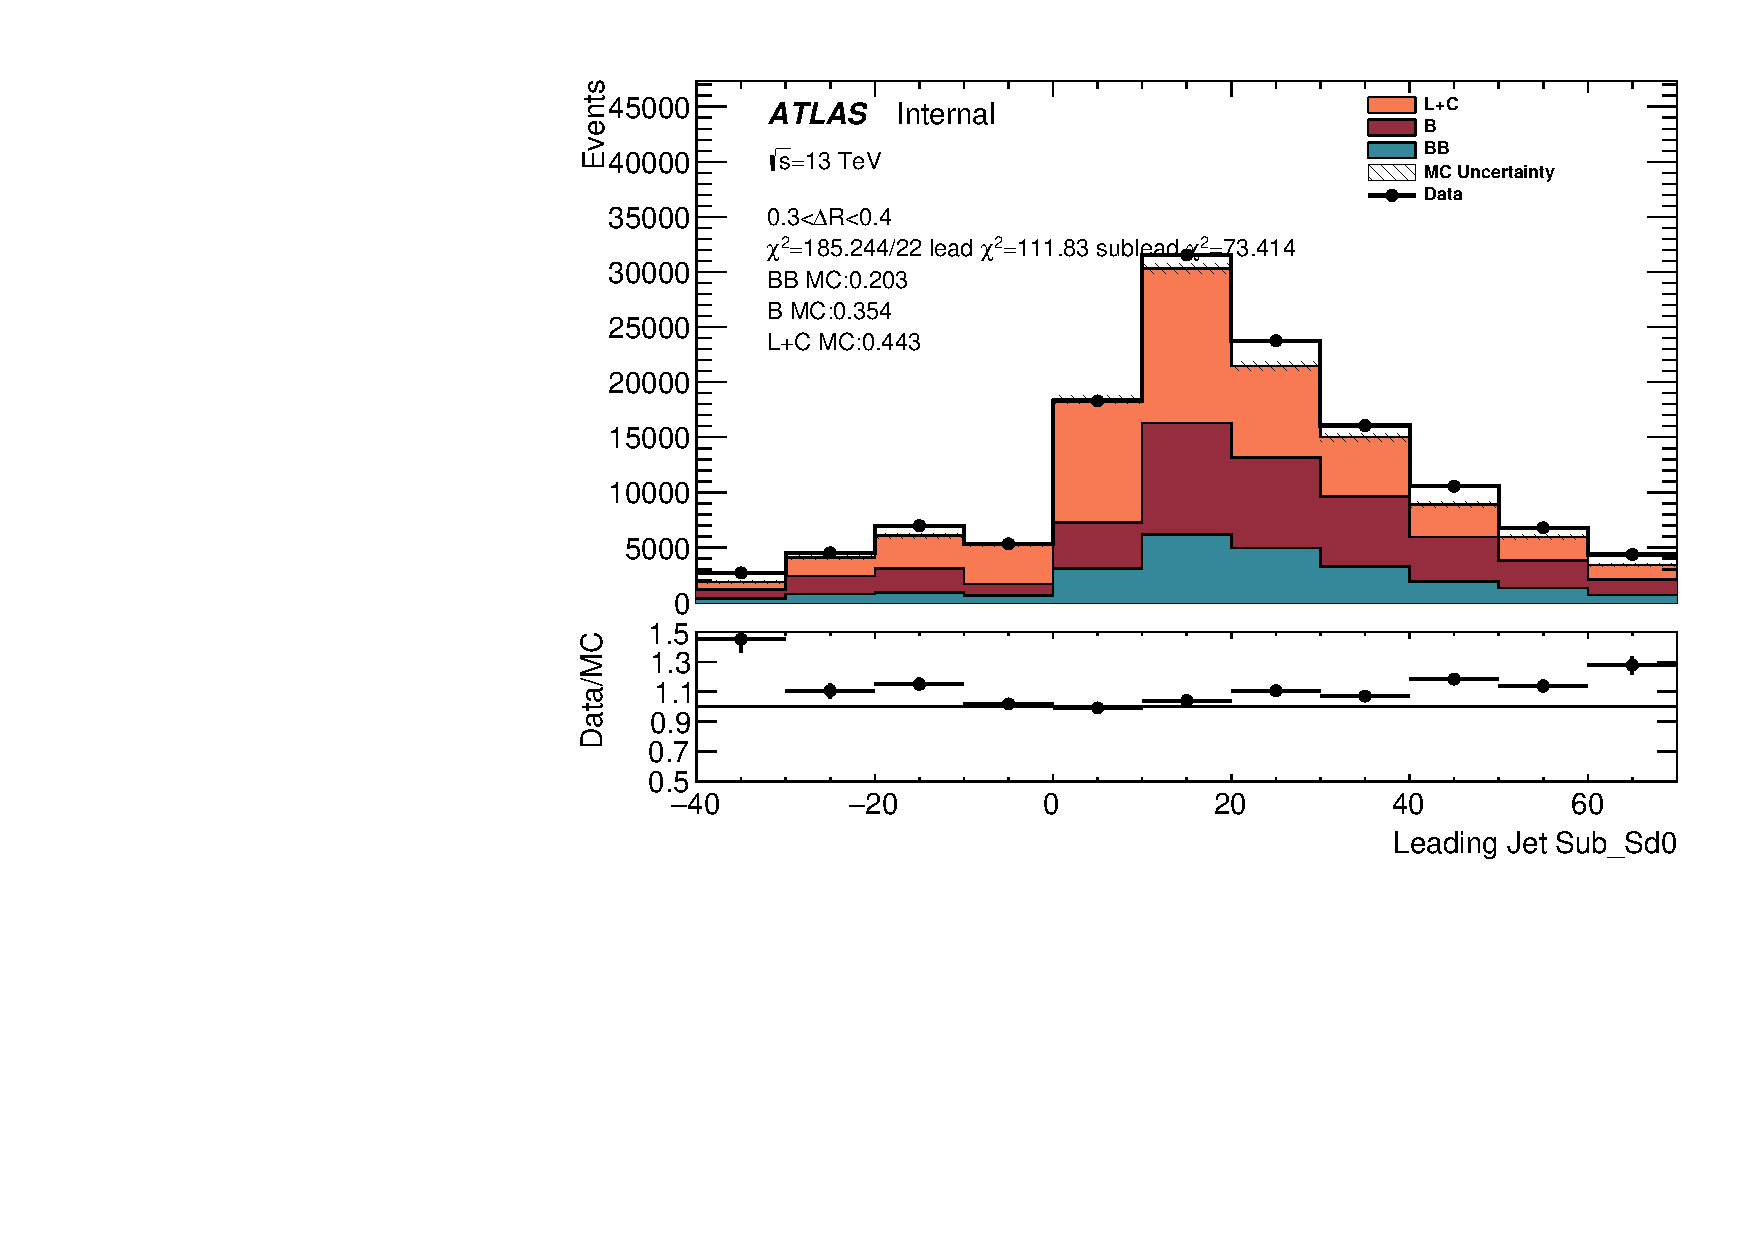
\includegraphics[width=0.32\textwidth]{figures/gbb/Sub_Sd0_Fits/Canv_PreFit_03-DeltaR-04_LpT_INF_SpT_INF_coarse_x.pdf}\\
 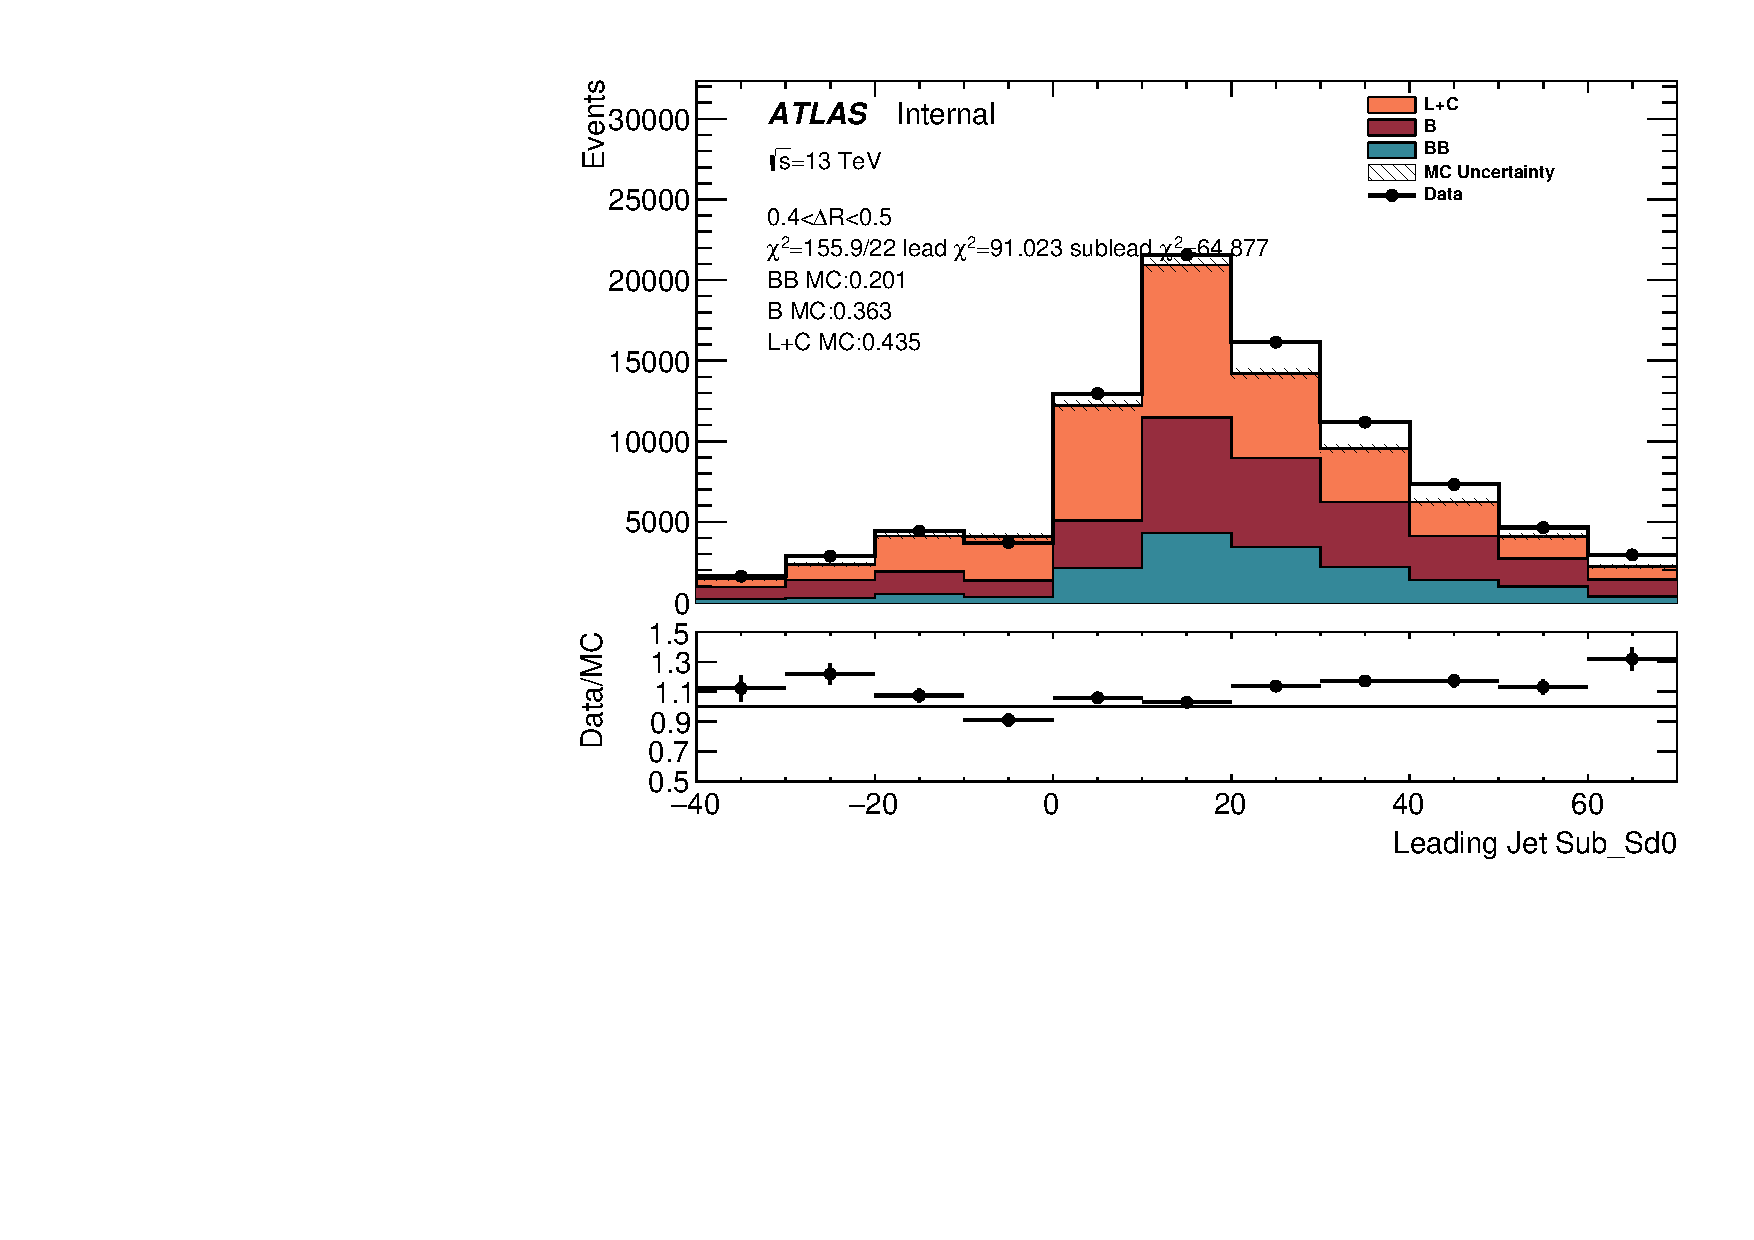
\includegraphics[width=0.32\textwidth]{figures/gbb/Sub_Sd0_Fits/Canv_PreFit_04-DeltaR-05_LpT_INF_SpT_INF_coarse_x.pdf}
 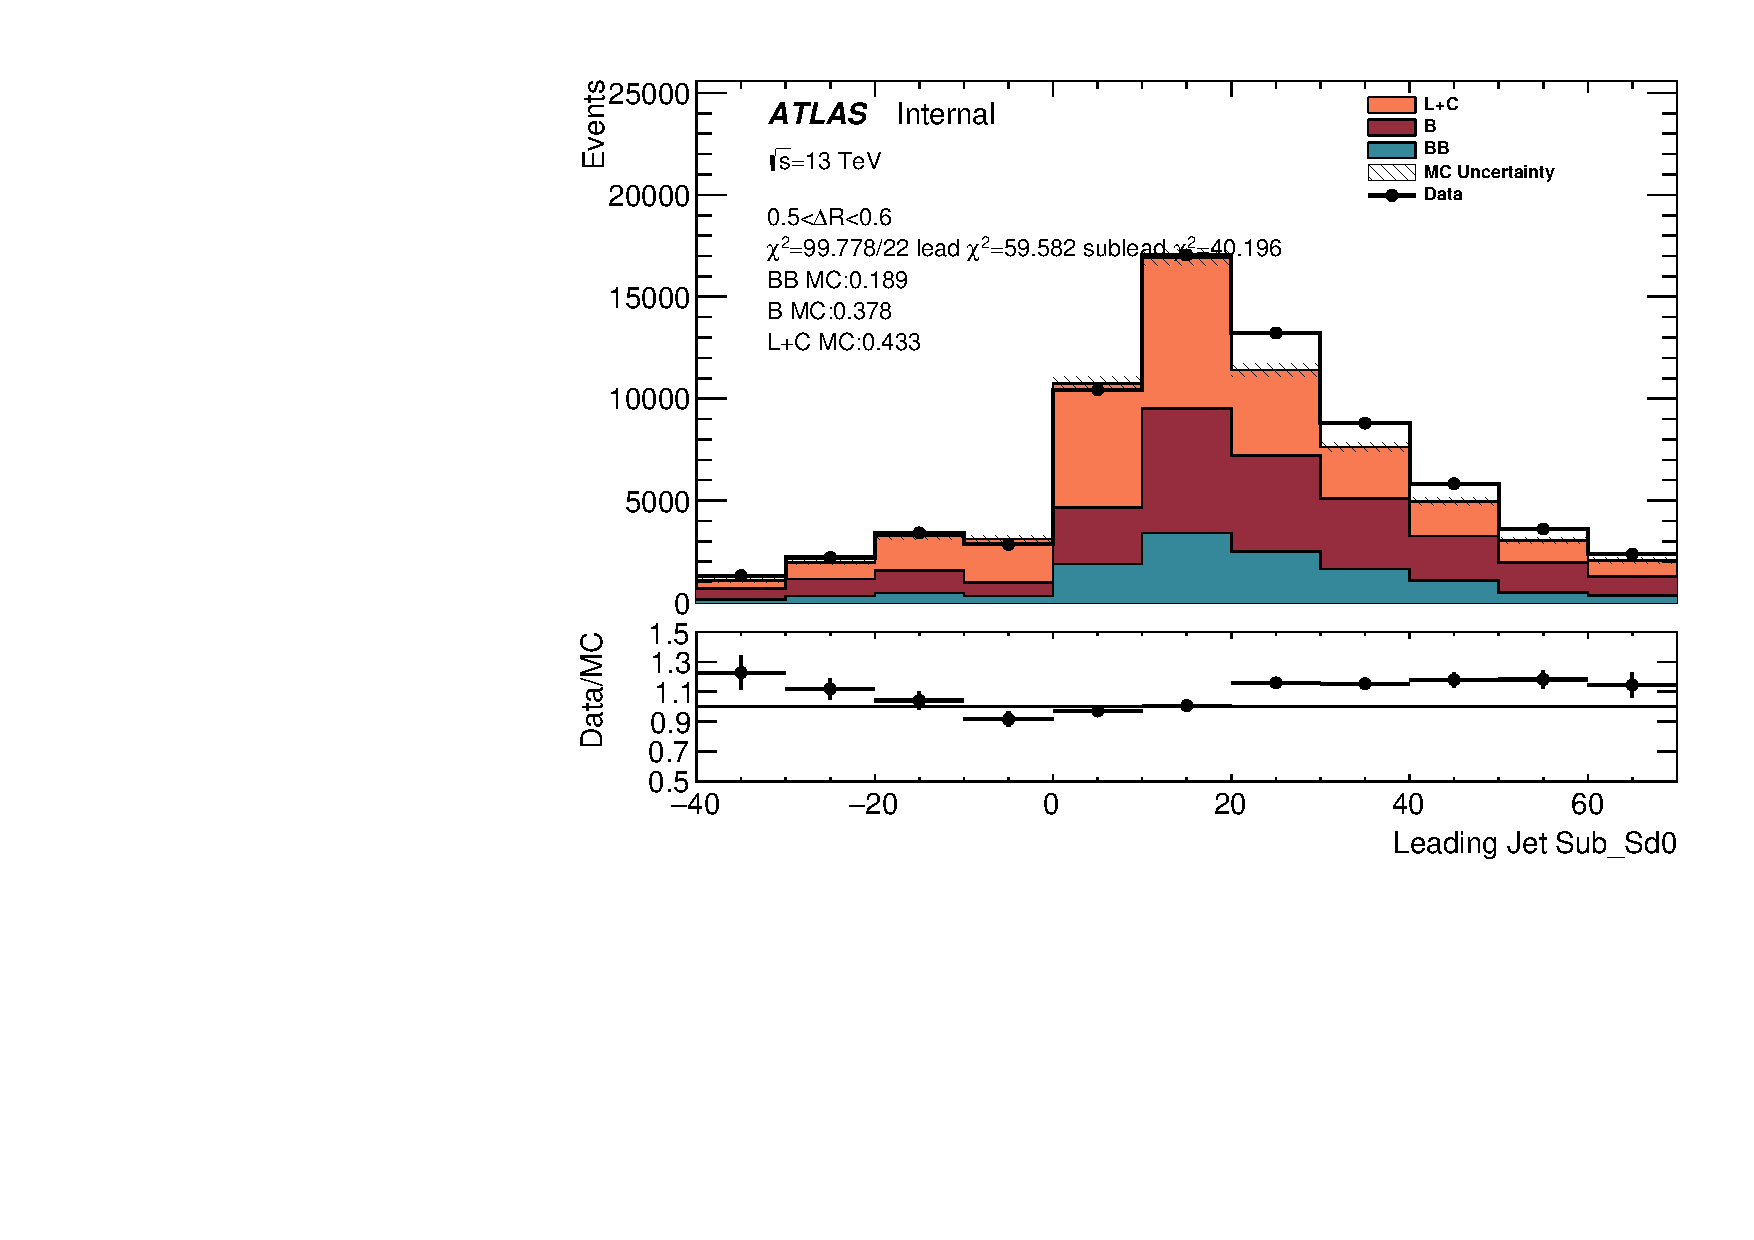
\includegraphics[width=0.32\textwidth]{figures/gbb/Sub_Sd0_Fits/Canv_PreFit_05-DeltaR-06_LpT_INF_SpT_INF_coarse_x.pdf}
 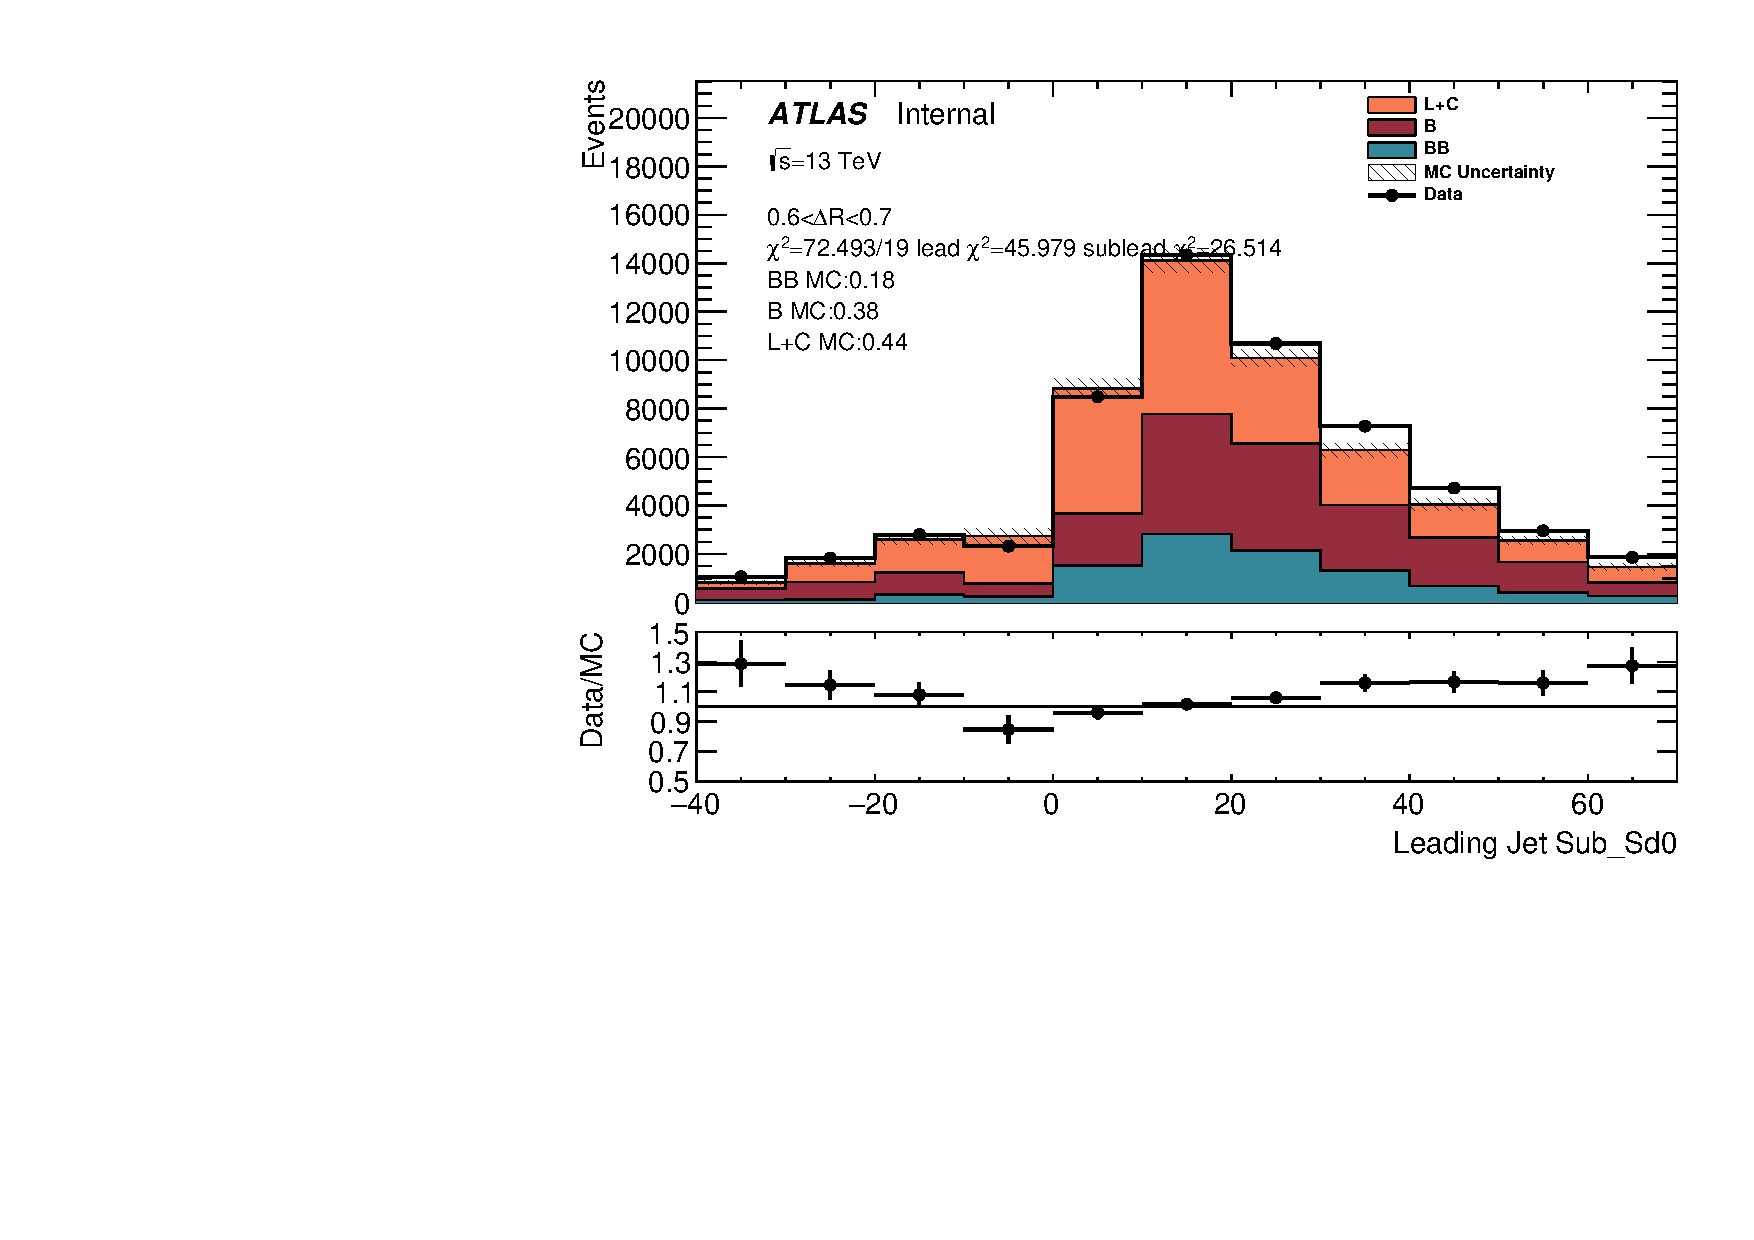
\includegraphics[width=0.32\textwidth]{figures/gbb/Sub_Sd0_Fits/Canv_PreFit_06-DeltaR-07_LpT_INF_SpT_INF_coarse_x.pdf}\\

\caption{Pre-fit \subsdzero distributions of the leading track jet in bins of $\Delta R$. }
  \label{fig:dR-prefits-leading}
\end{figure}


\begin{figure}[htbp]
  \centering
 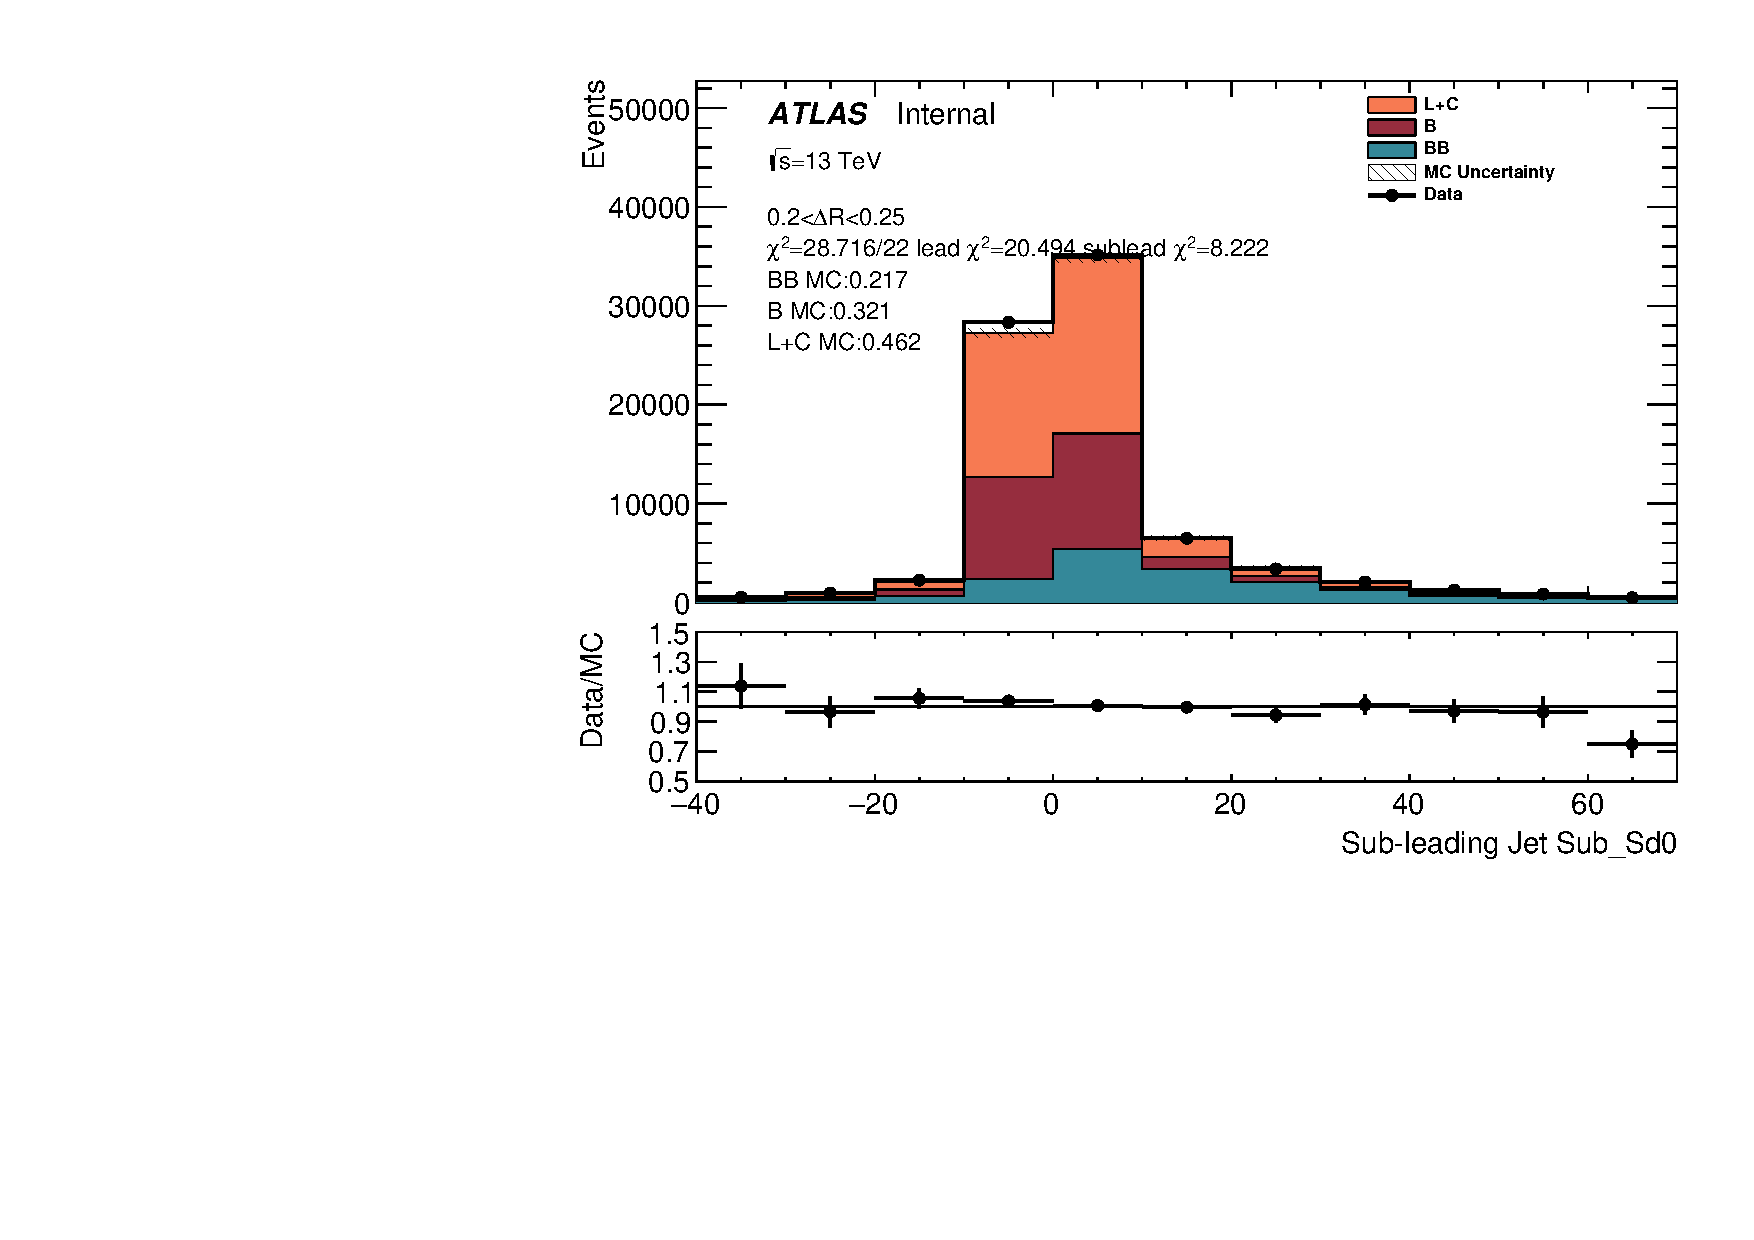
\includegraphics[width=0.32\textwidth]{figures/gbb/Sub_Sd0_Fits/Canv_PreFit_02-DeltaR-025_LpT_INF_SpT_INF_coarse_y.pdf}
 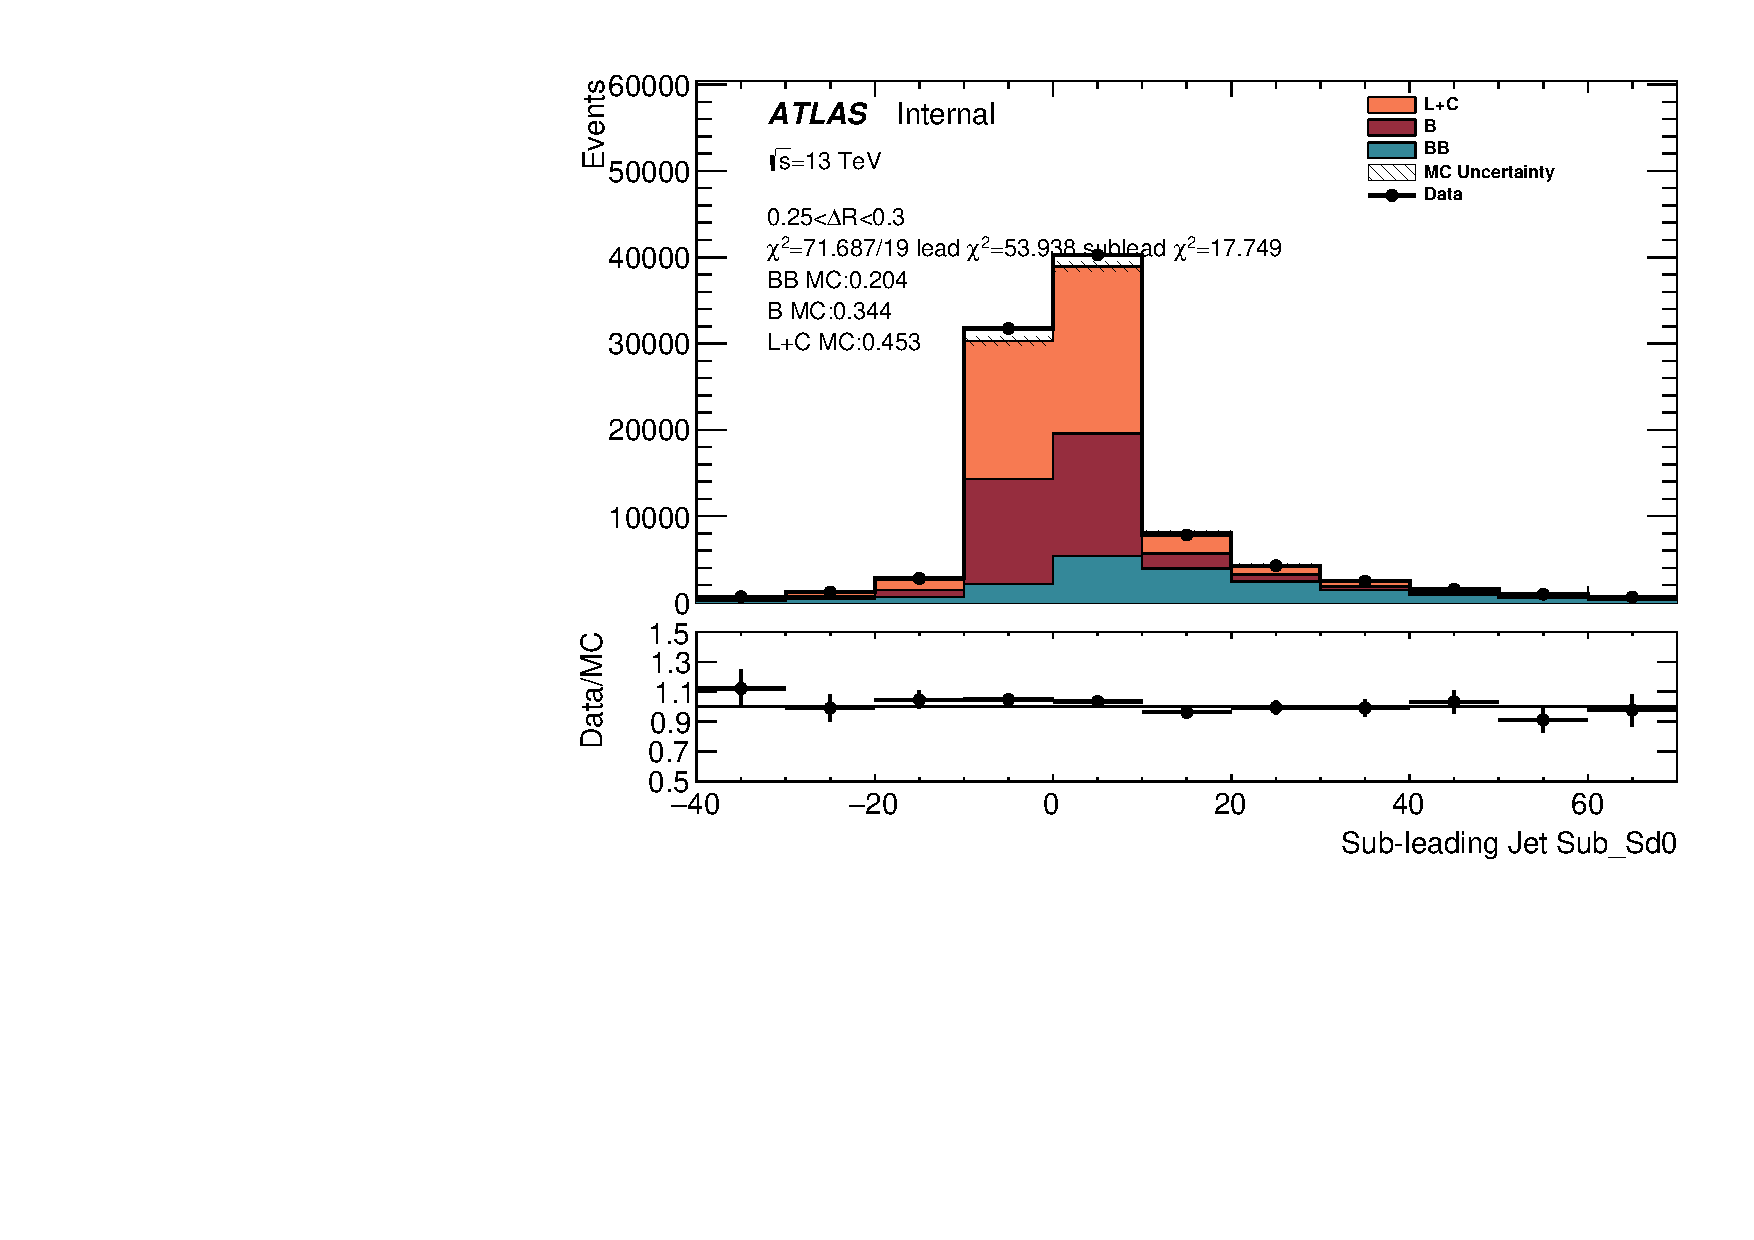
\includegraphics[width=0.32\textwidth]{figures/gbb/Sub_Sd0_Fits/Canv_PreFit_025-DeltaR-03_LpT_INF_SpT_INF_coarse_y.pdf}
 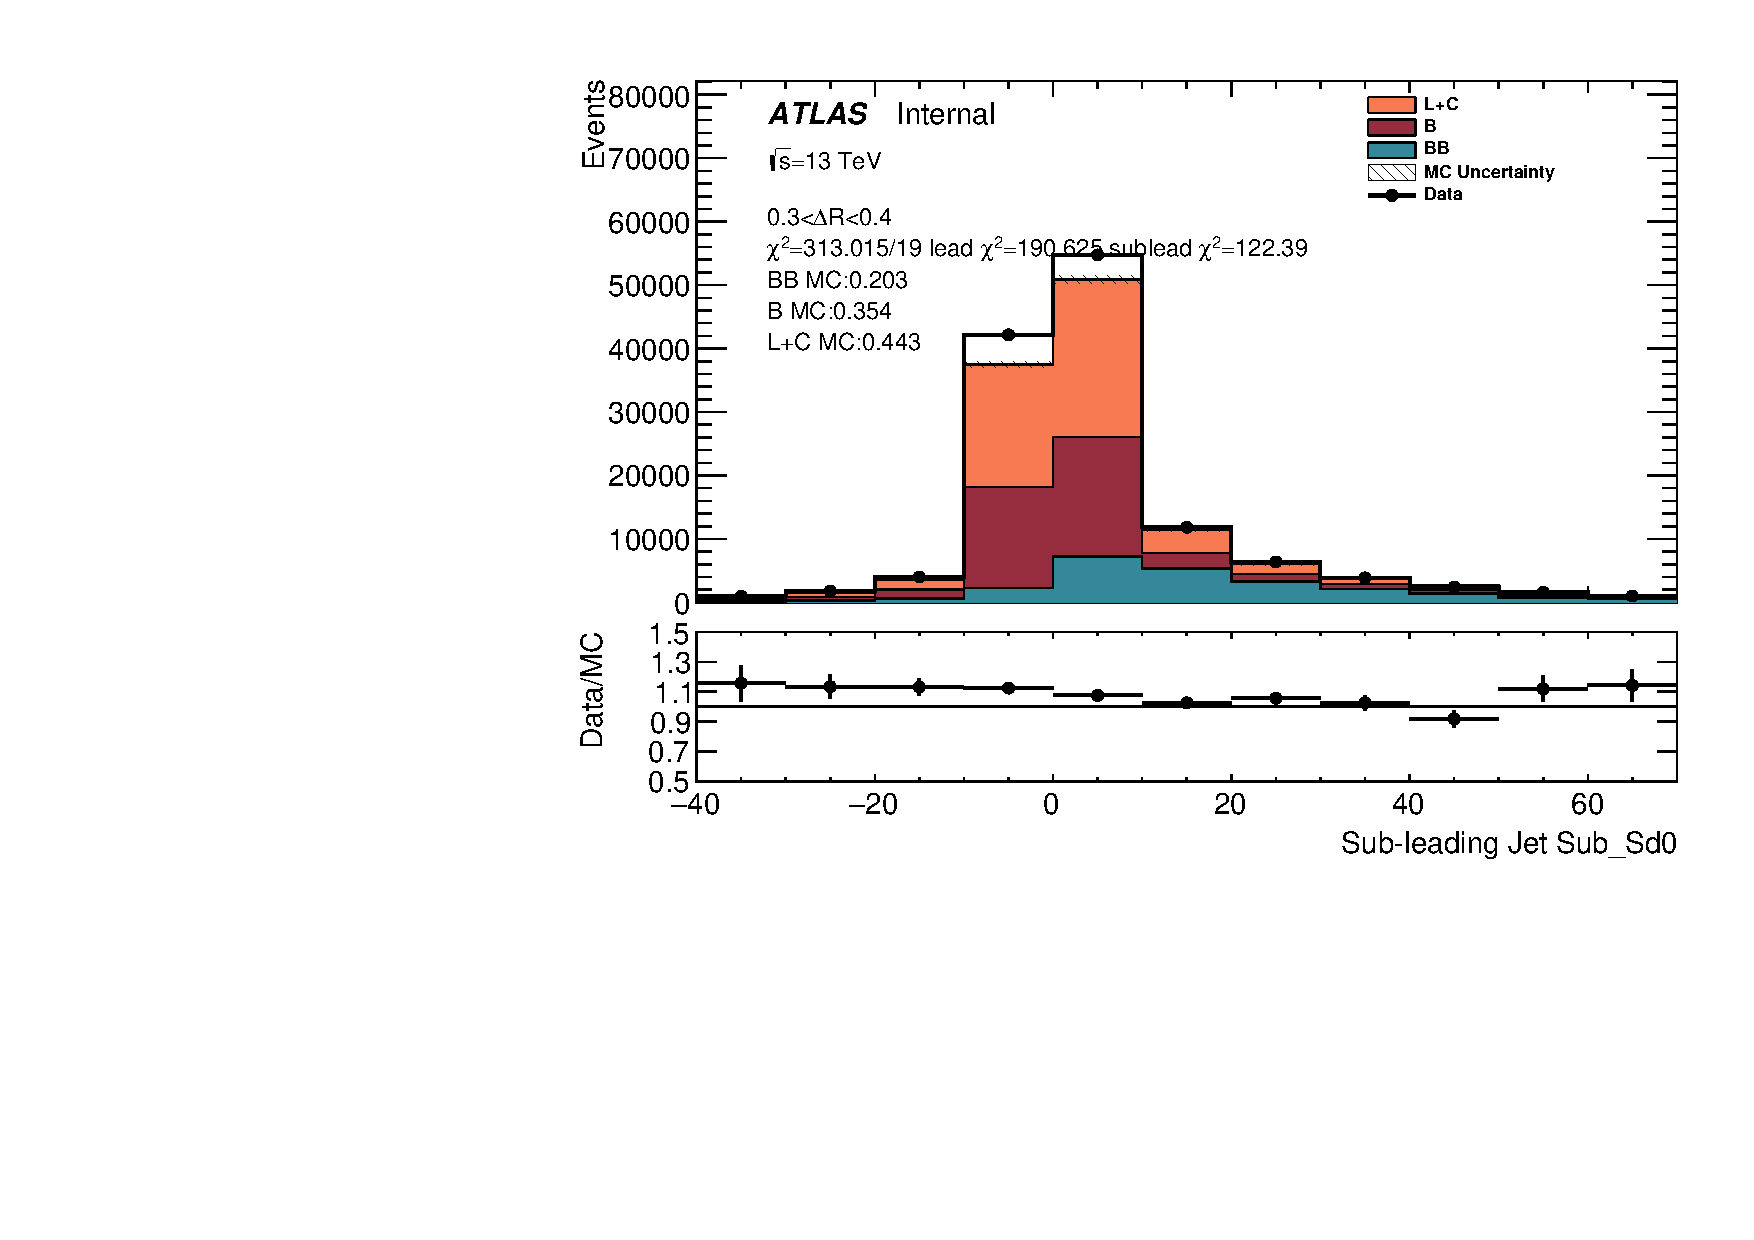
\includegraphics[width=0.32\textwidth]{figures/gbb/Sub_Sd0_Fits/Canv_PreFit_03-DeltaR-04_LpT_INF_SpT_INF_coarse_y.pdf}\\
 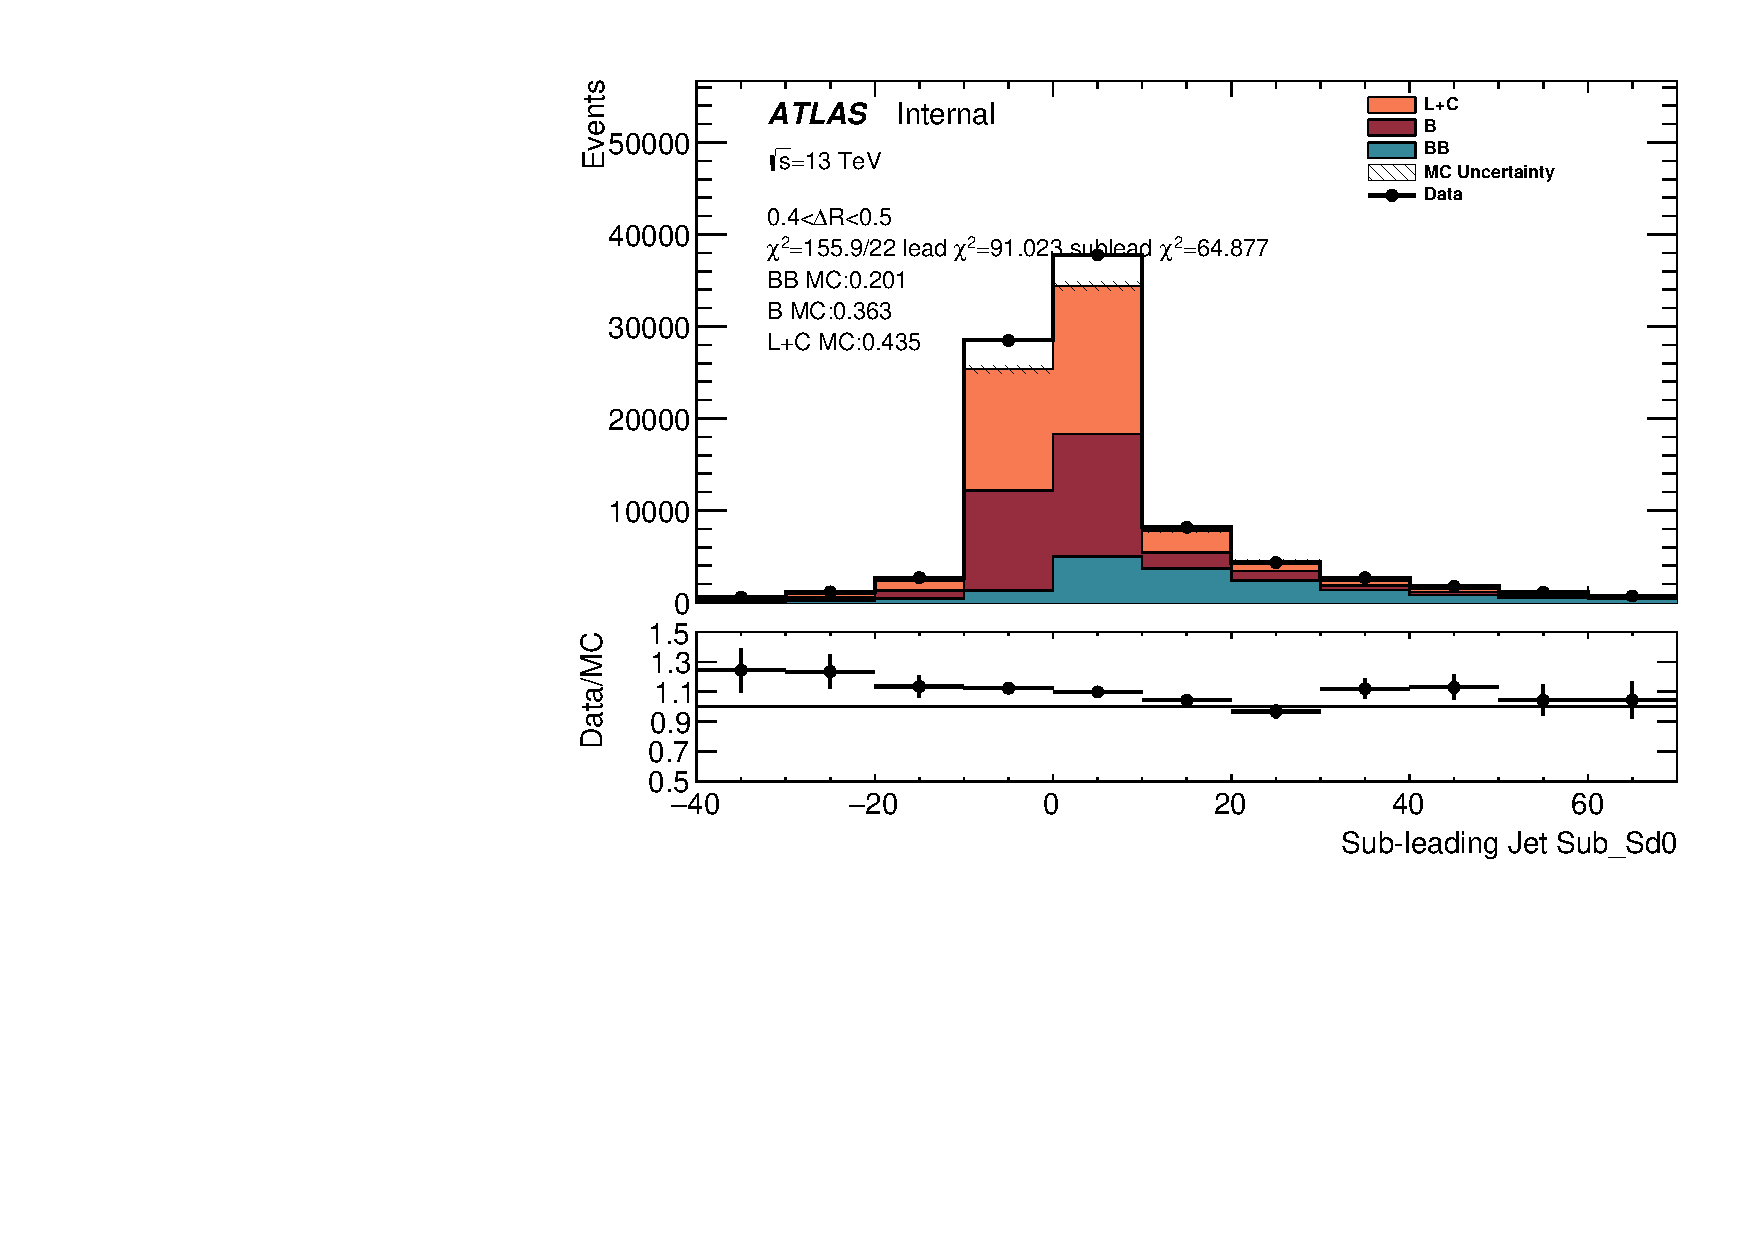
\includegraphics[width=0.32\textwidth]{figures/gbb/Sub_Sd0_Fits/Canv_PreFit_04-DeltaR-05_LpT_INF_SpT_INF_coarse_y.pdf}
 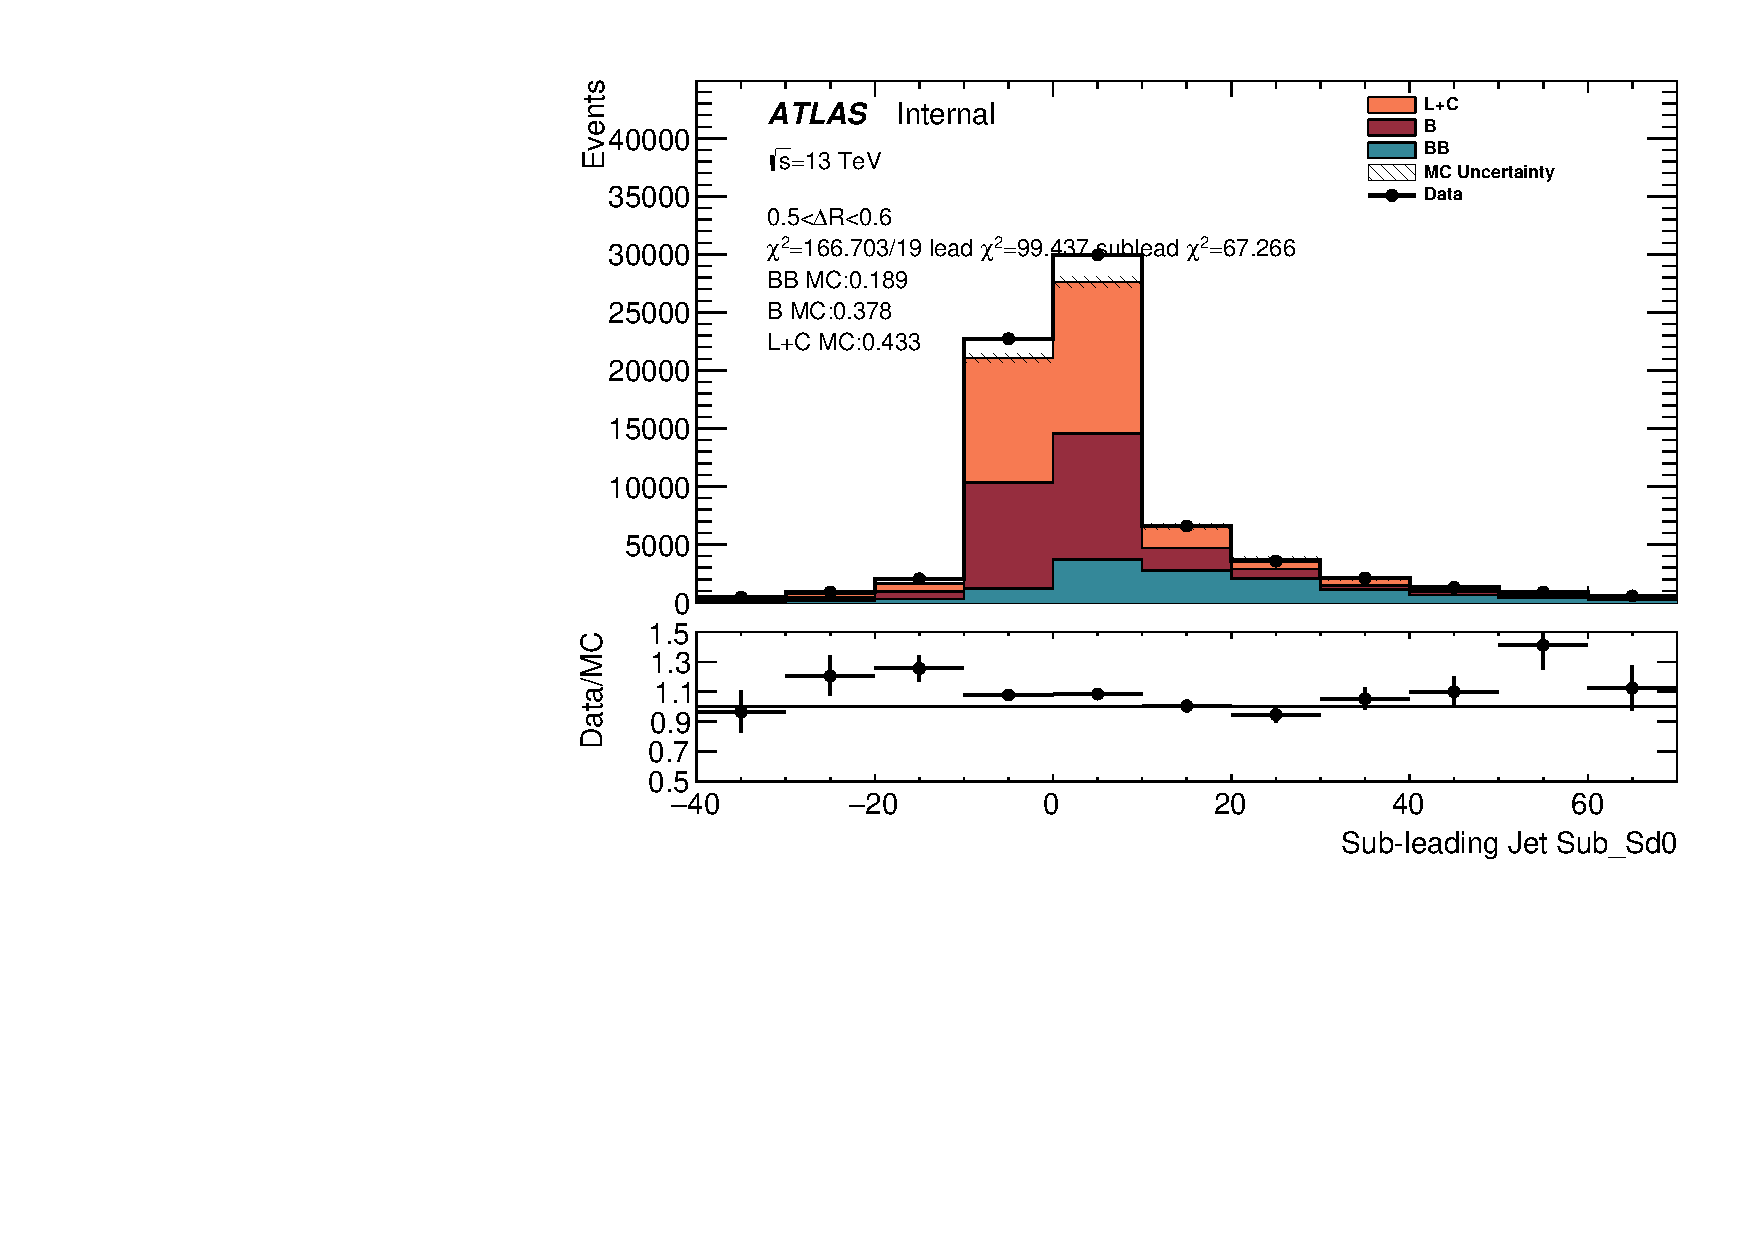
\includegraphics[width=0.32\textwidth]{figures/gbb/Sub_Sd0_Fits/Canv_PreFit_05-DeltaR-06_LpT_INF_SpT_INF_coarse_y.pdf}
 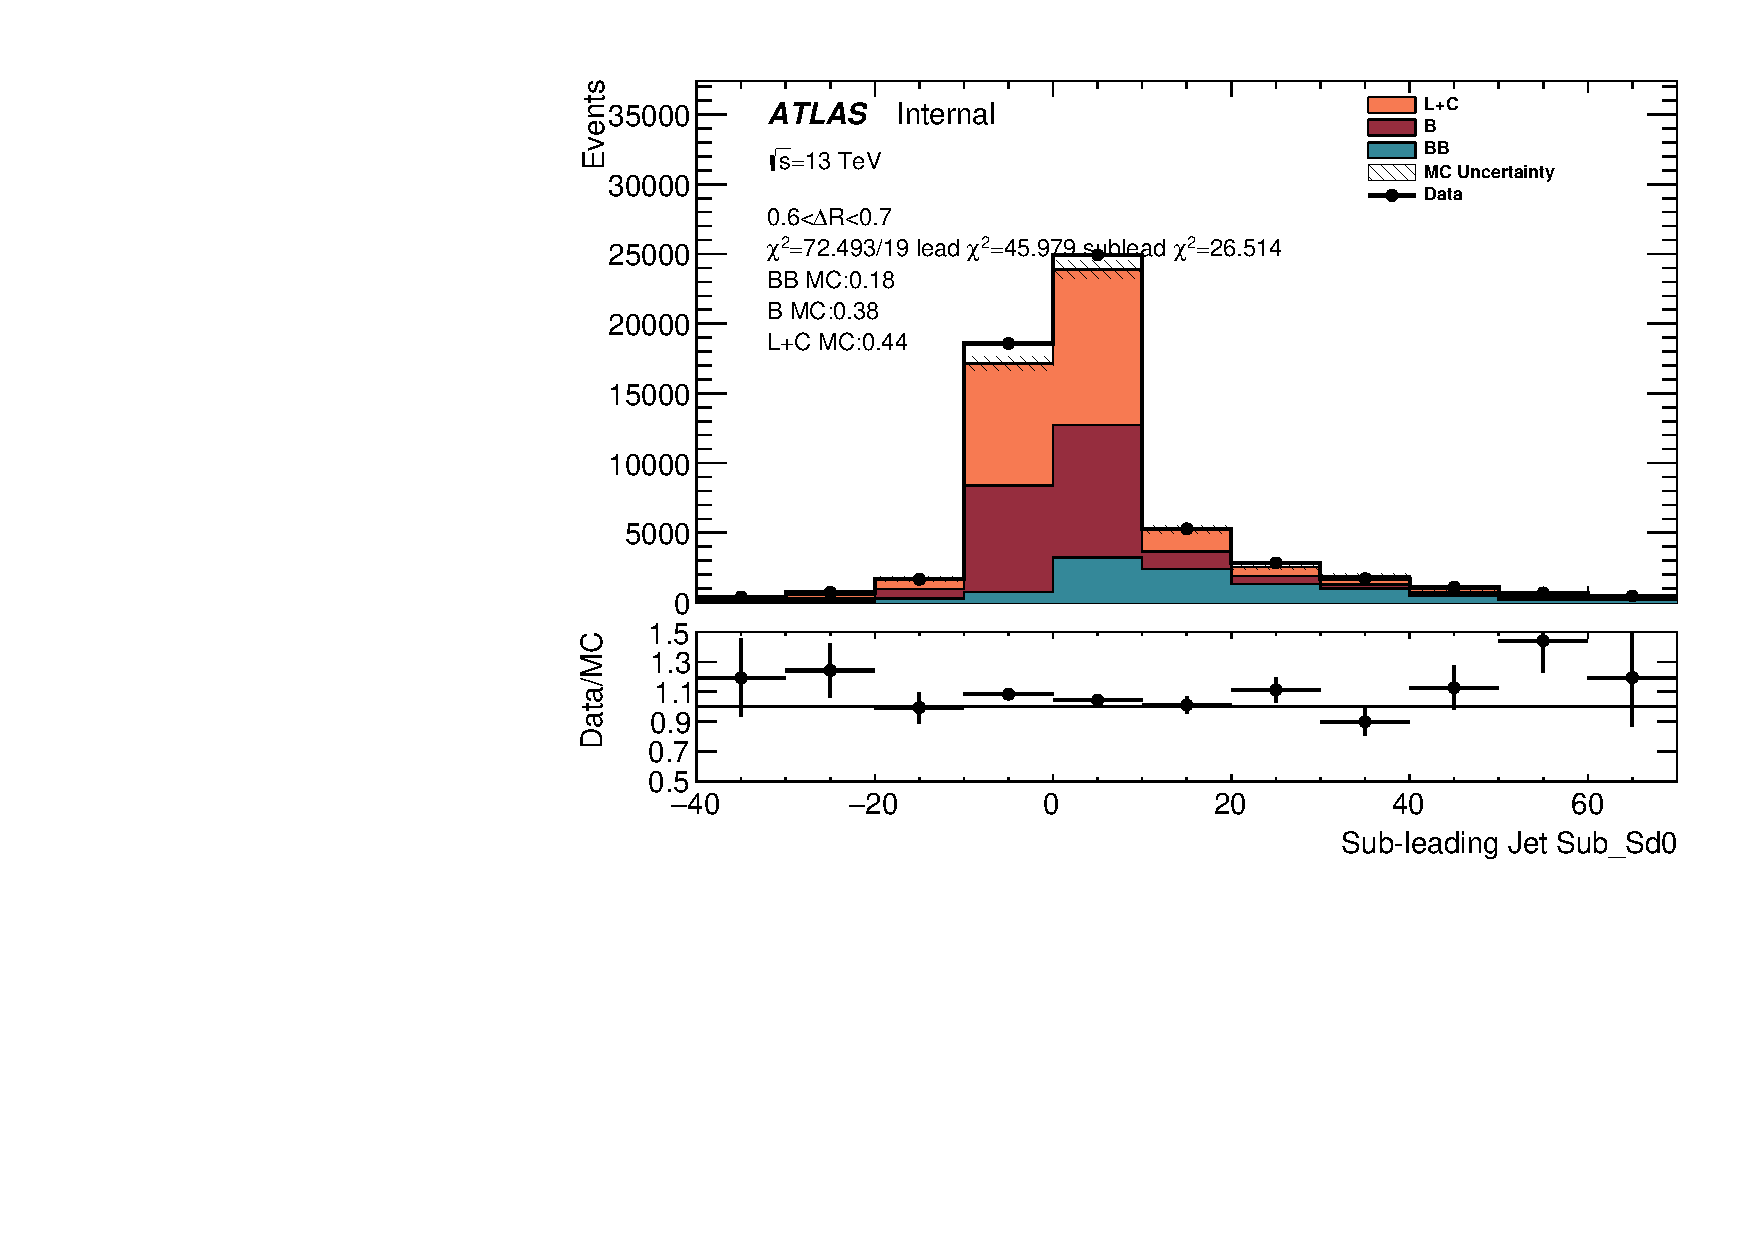
\includegraphics[width=0.32\textwidth]{figures/gbb/Sub_Sd0_Fits/Canv_PreFit_06-DeltaR-07_LpT_INF_SpT_INF_coarse_y.pdf}\\

\caption{Pre-fit \subsdzero distributions of the sub-leading track jet in bins of $\Delta R$. }
  \label{fig:dR-prefits-subleading}
\end{figure}

\begin{figure}[htbp]
  \centering
 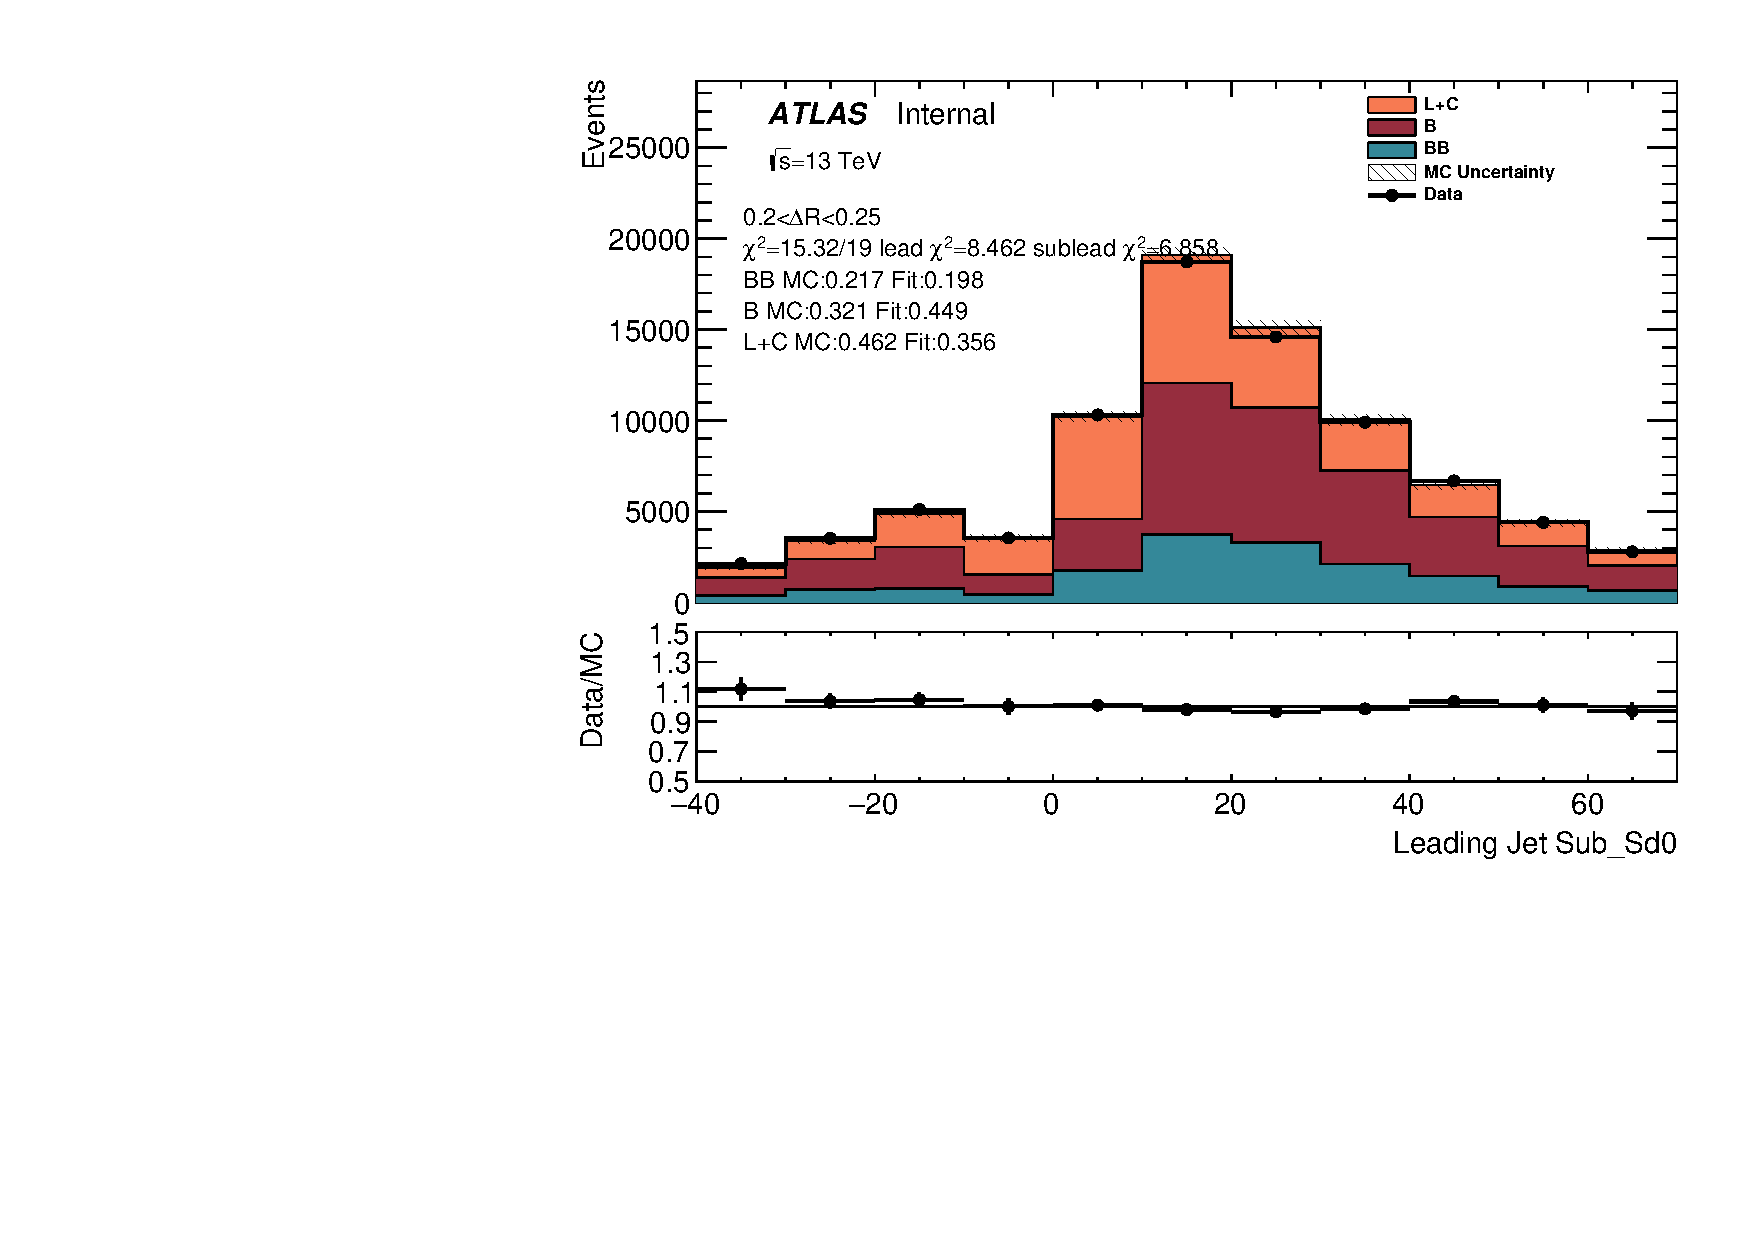
\includegraphics[width=0.32\textwidth]{figures/gbb/Sub_Sd0_Fits/Canv_Fit_02-DeltaR-025_LpT_INF_SpT_INF_coarse_x.pdf}
 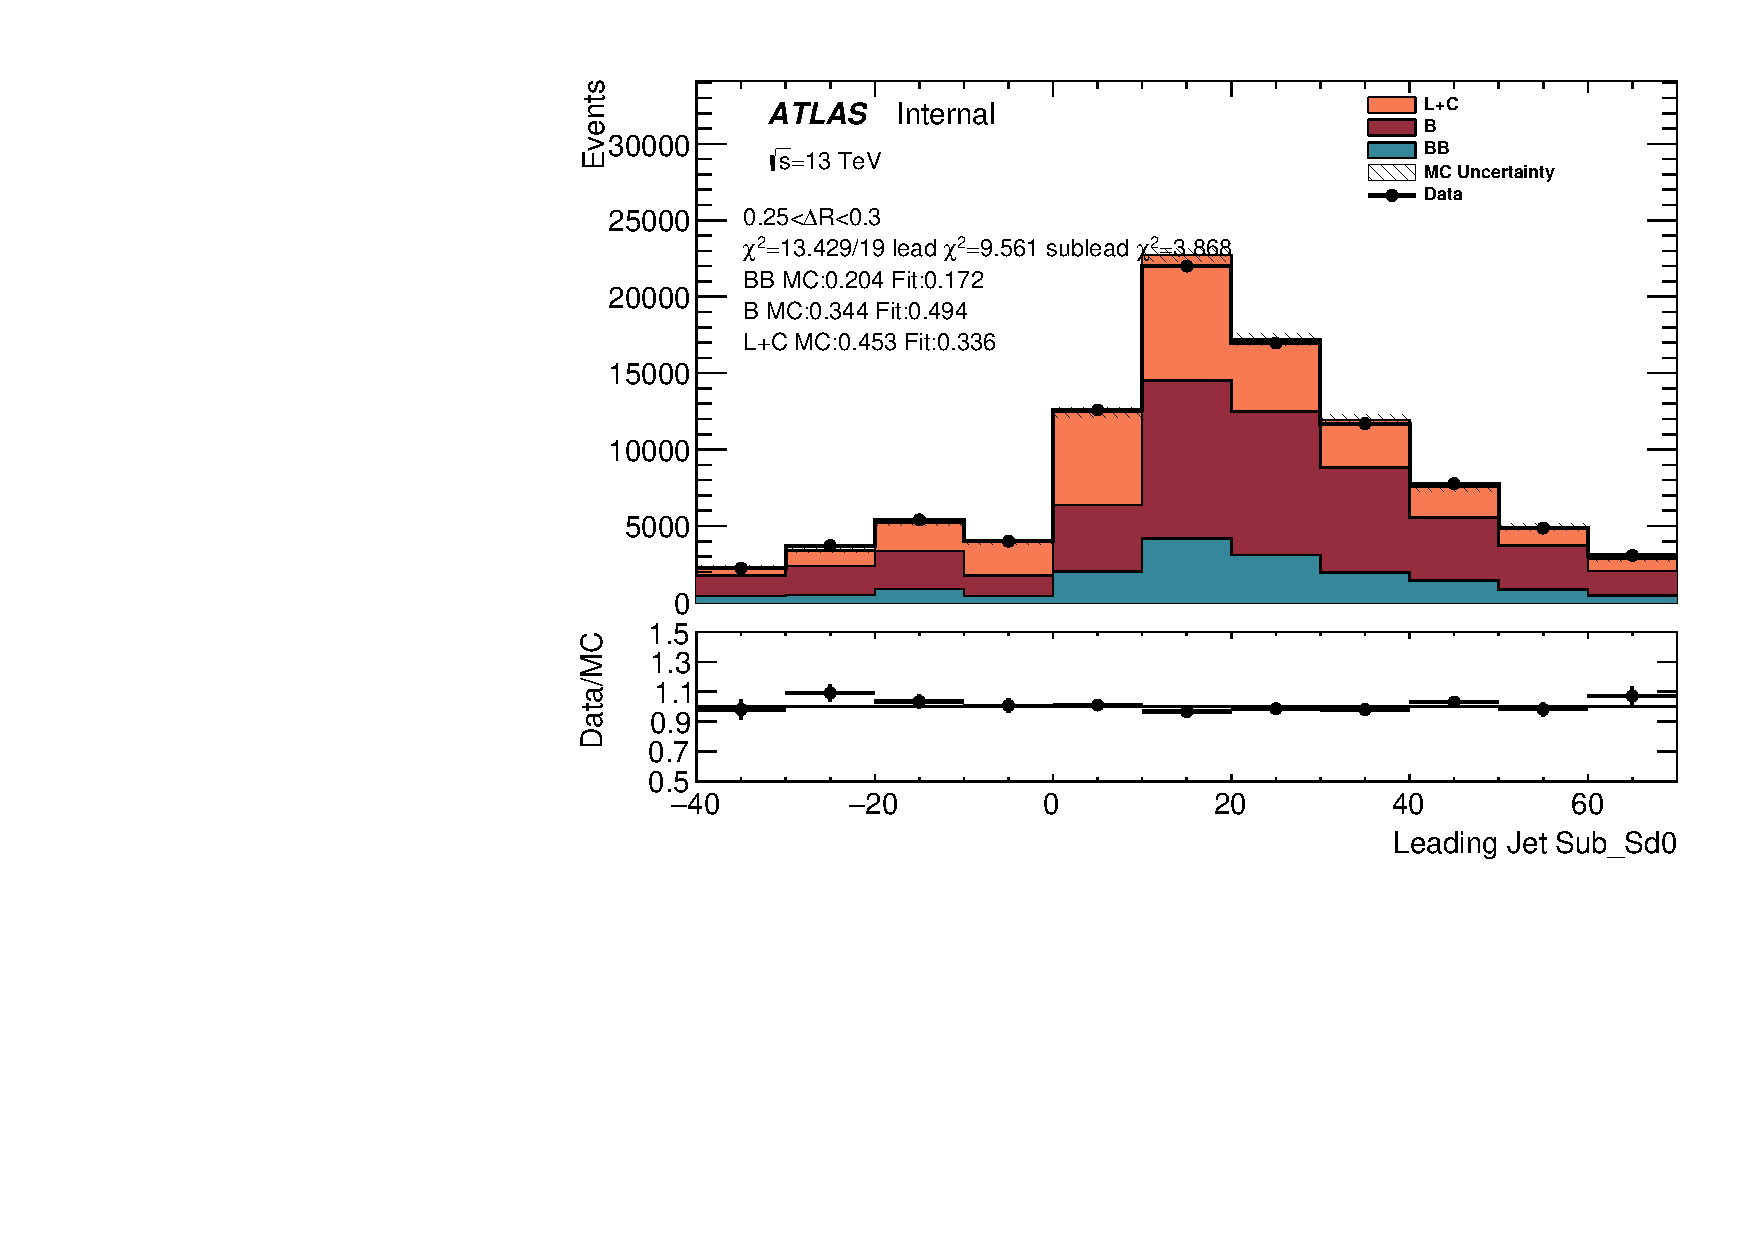
\includegraphics[width=0.32\textwidth]{figures/gbb/Sub_Sd0_Fits/Canv_Fit_025-DeltaR-03_LpT_INF_SpT_INF_coarse_x.pdf}
 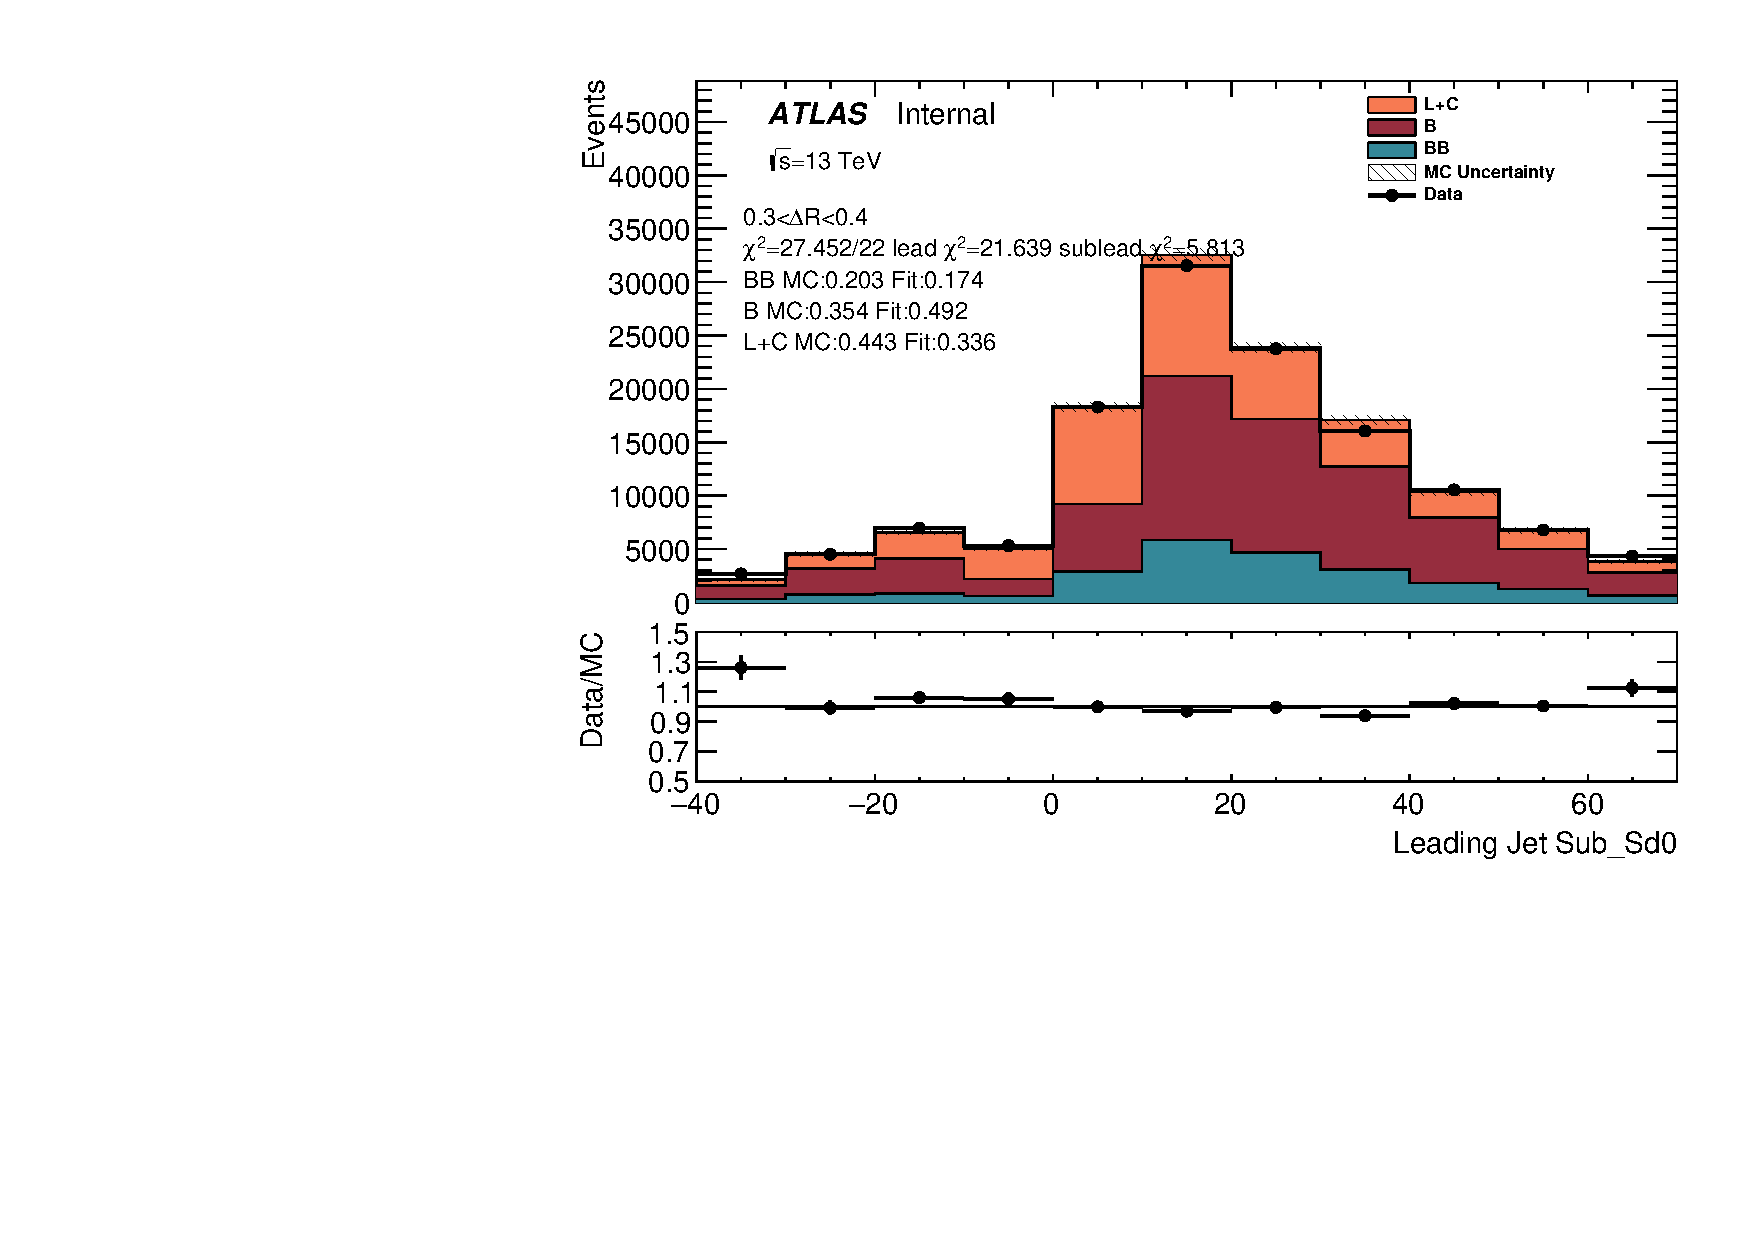
\includegraphics[width=0.32\textwidth]{figures/gbb/Sub_Sd0_Fits/Canv_Fit_03-DeltaR-04_LpT_INF_SpT_INF_coarse_x.pdf}\\
 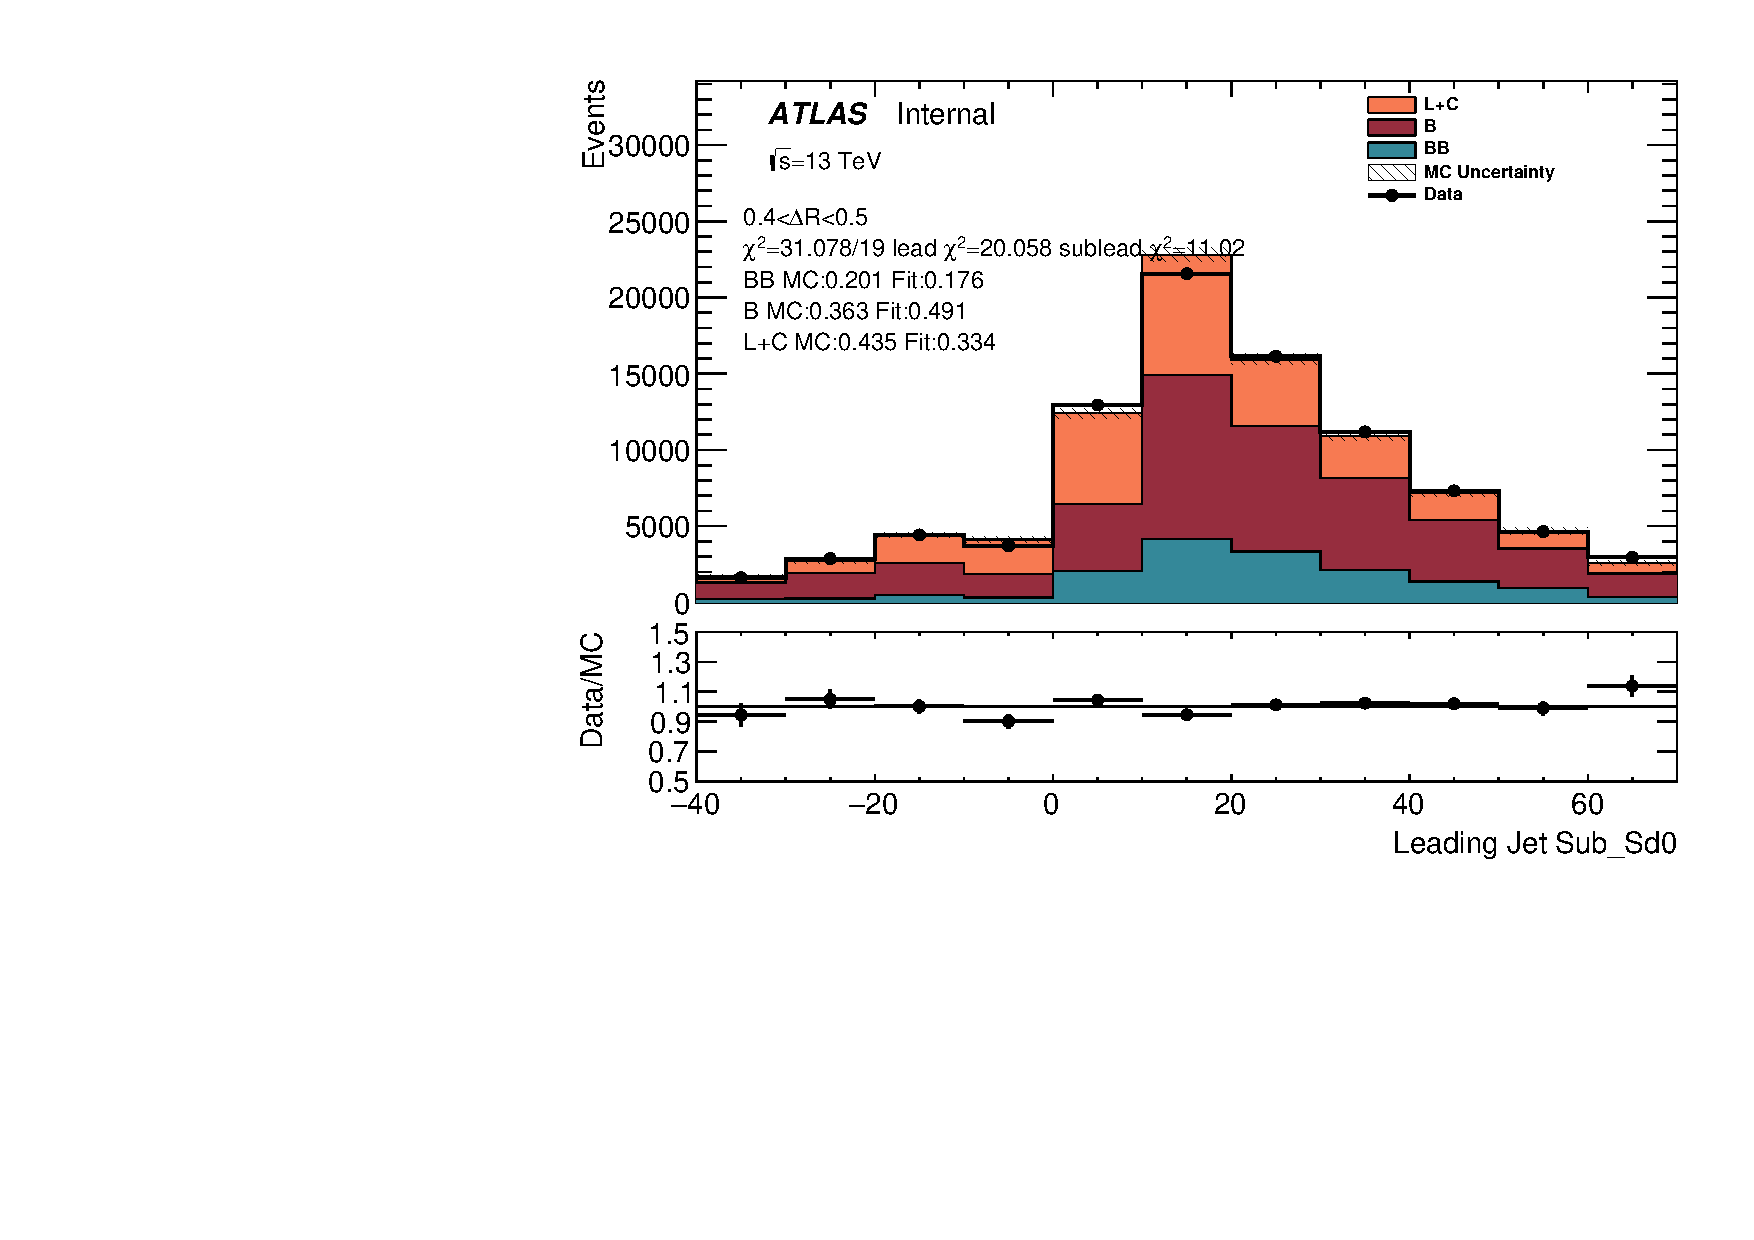
\includegraphics[width=0.32\textwidth]{figures/gbb/Sub_Sd0_Fits/Canv_Fit_04-DeltaR-05_LpT_INF_SpT_INF_coarse_x.pdf}
 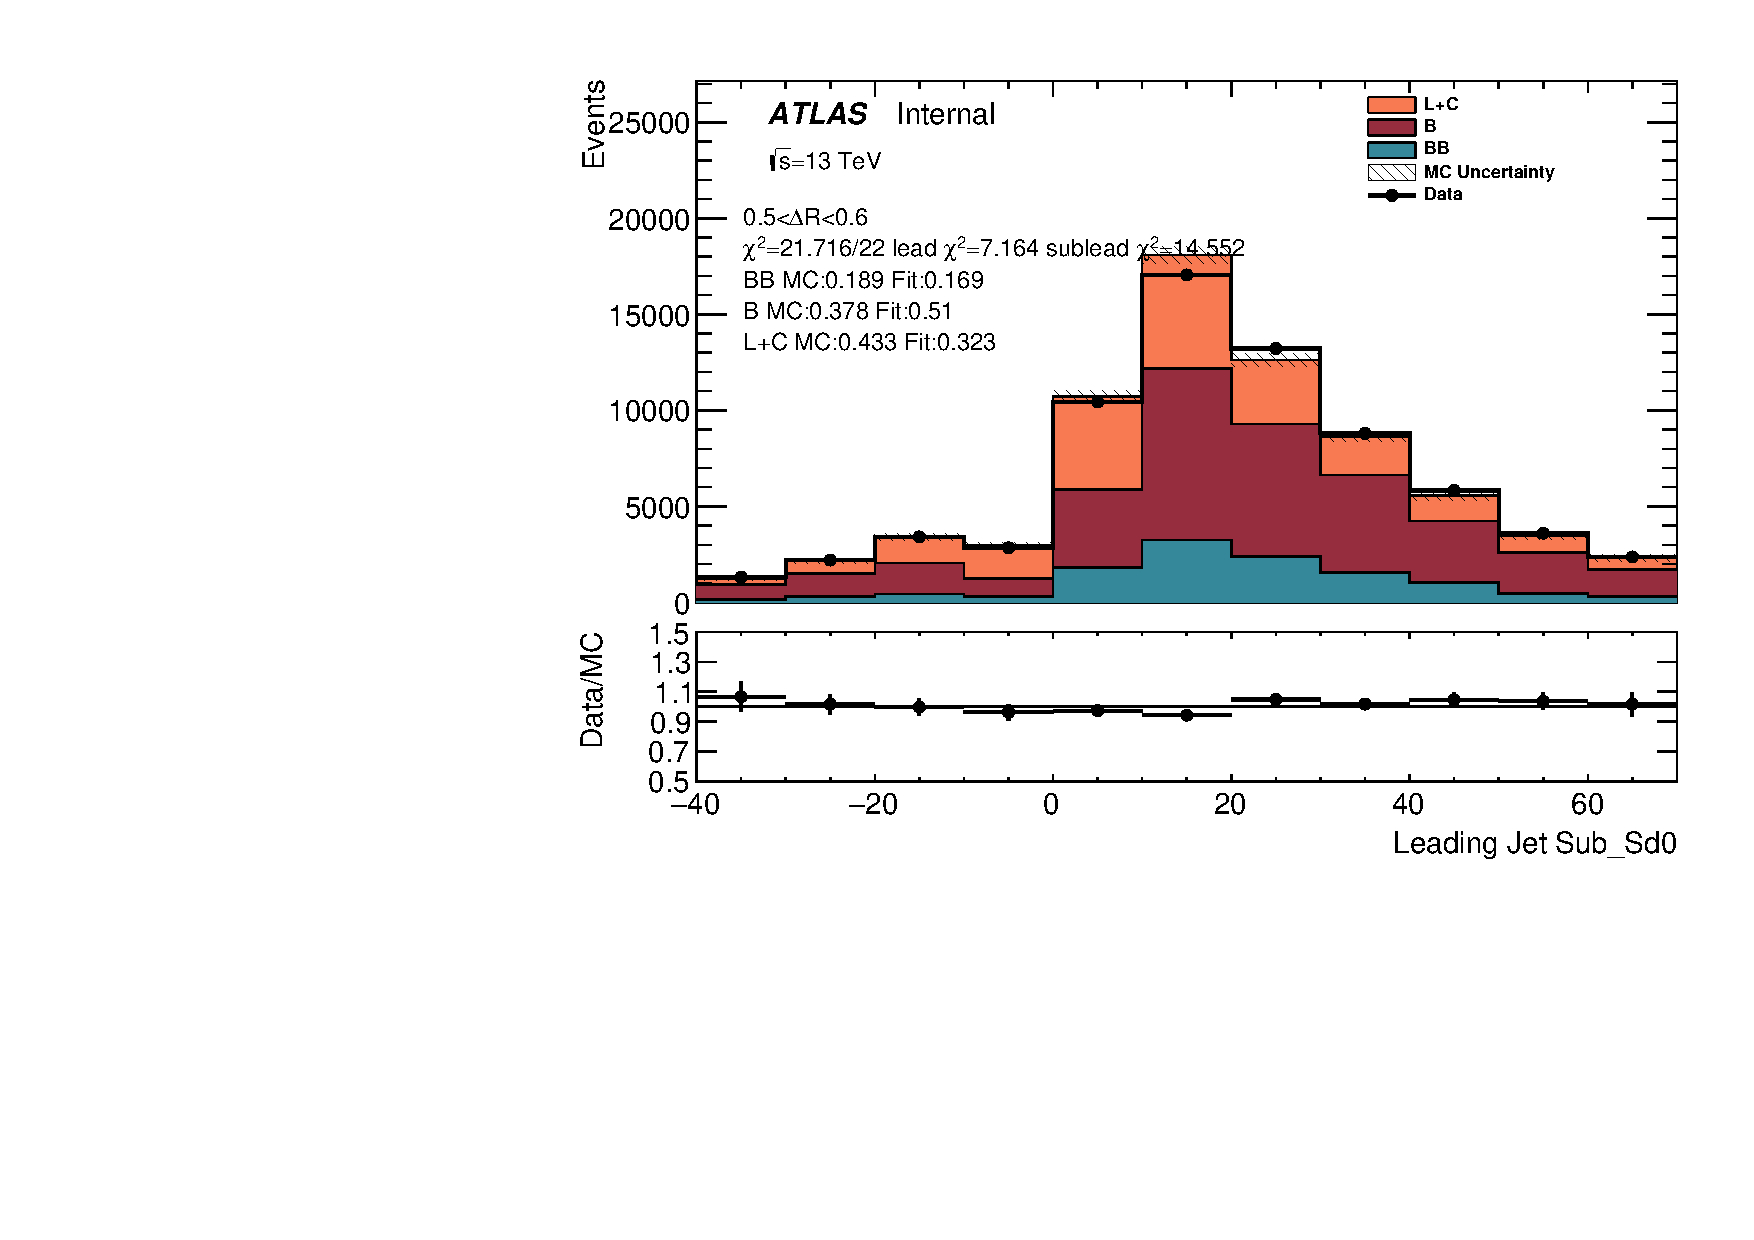
\includegraphics[width=0.32\textwidth]{figures/gbb/Sub_Sd0_Fits/Canv_Fit_05-DeltaR-06_LpT_INF_SpT_INF_coarse_x.pdf}
 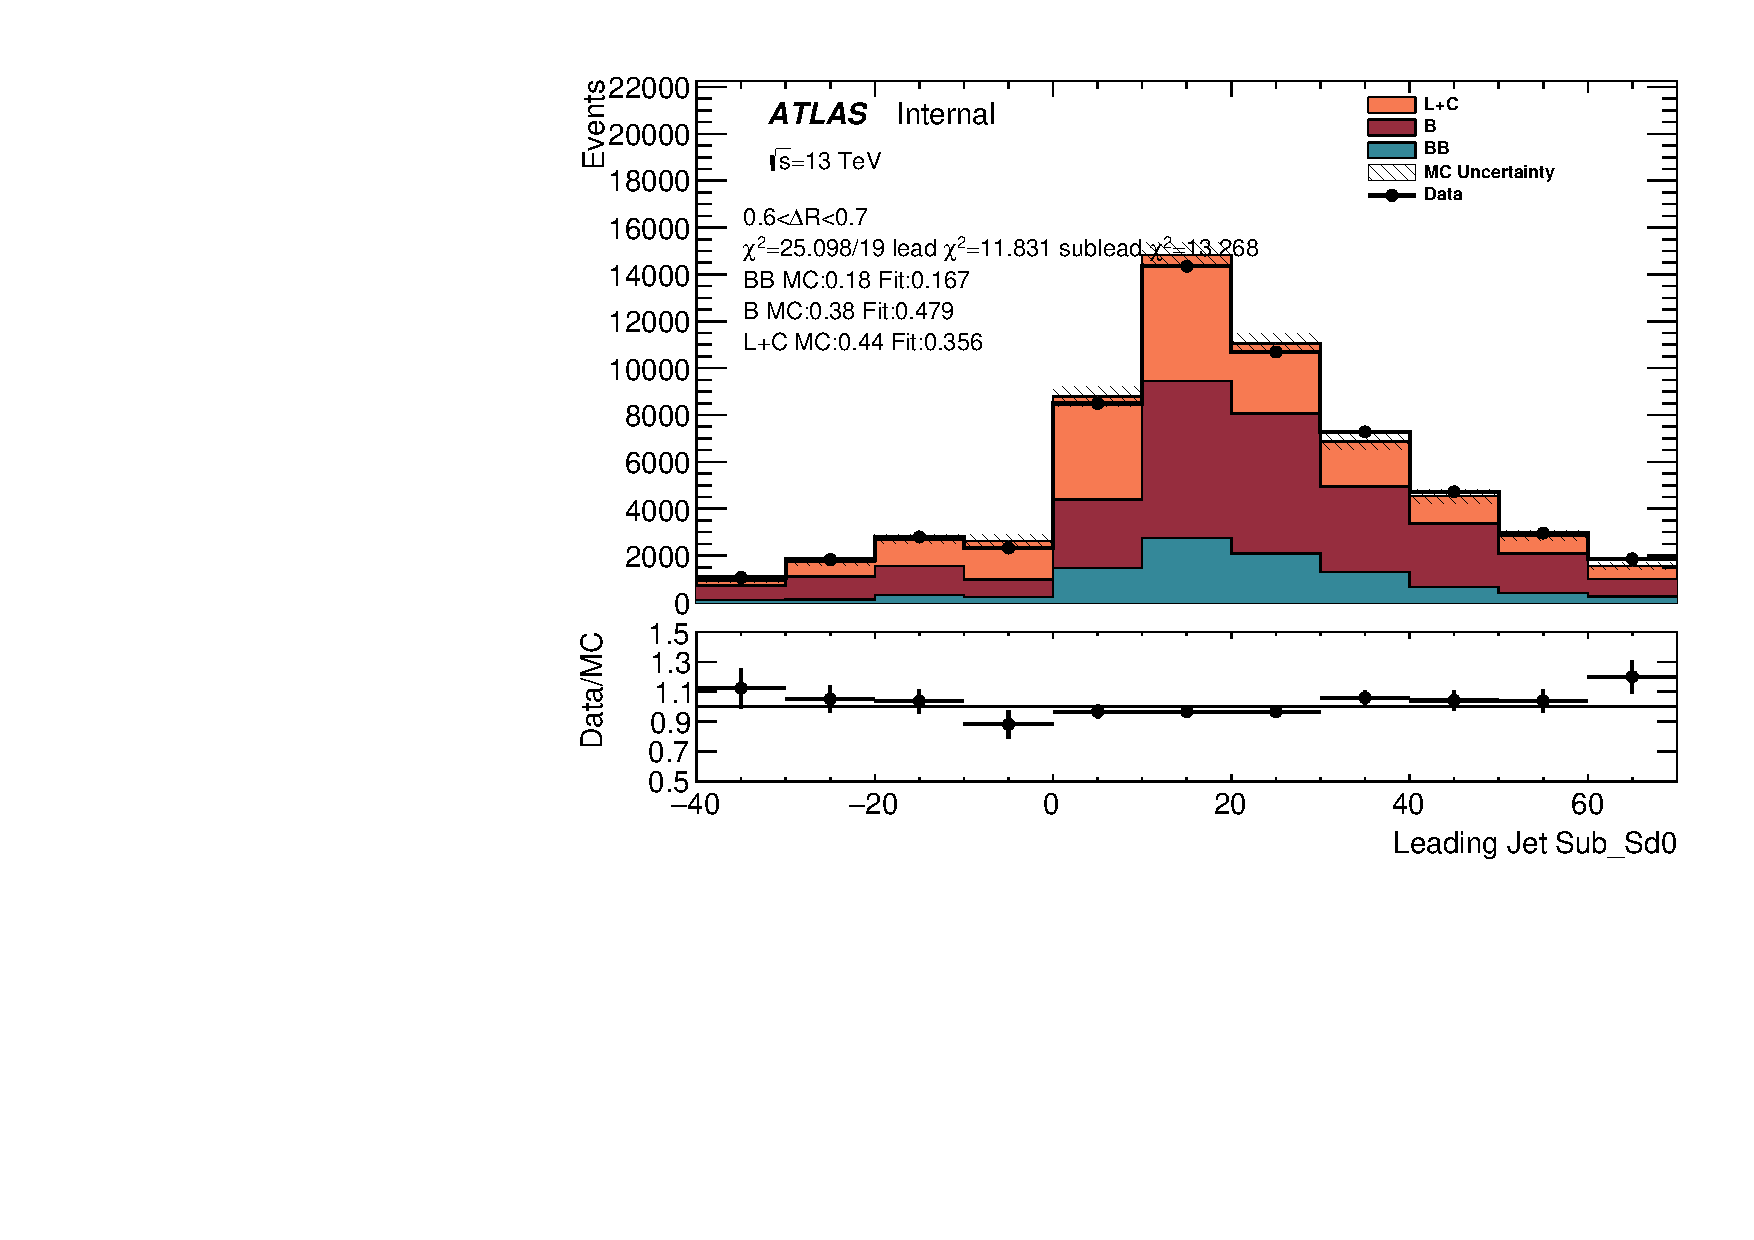
\includegraphics[width=0.32\textwidth]{figures/gbb/Sub_Sd0_Fits/Canv_Fit_06-DeltaR-07_LpT_INF_SpT_INF_coarse_x.pdf}\\


\caption{Post-fit \subsdzero distributions of the leading track jet in bins of $\Delta R$. }
  \label{fig:dR-postfits-leading}
\end{figure}


\begin{figure}[htbp]
  \centering
 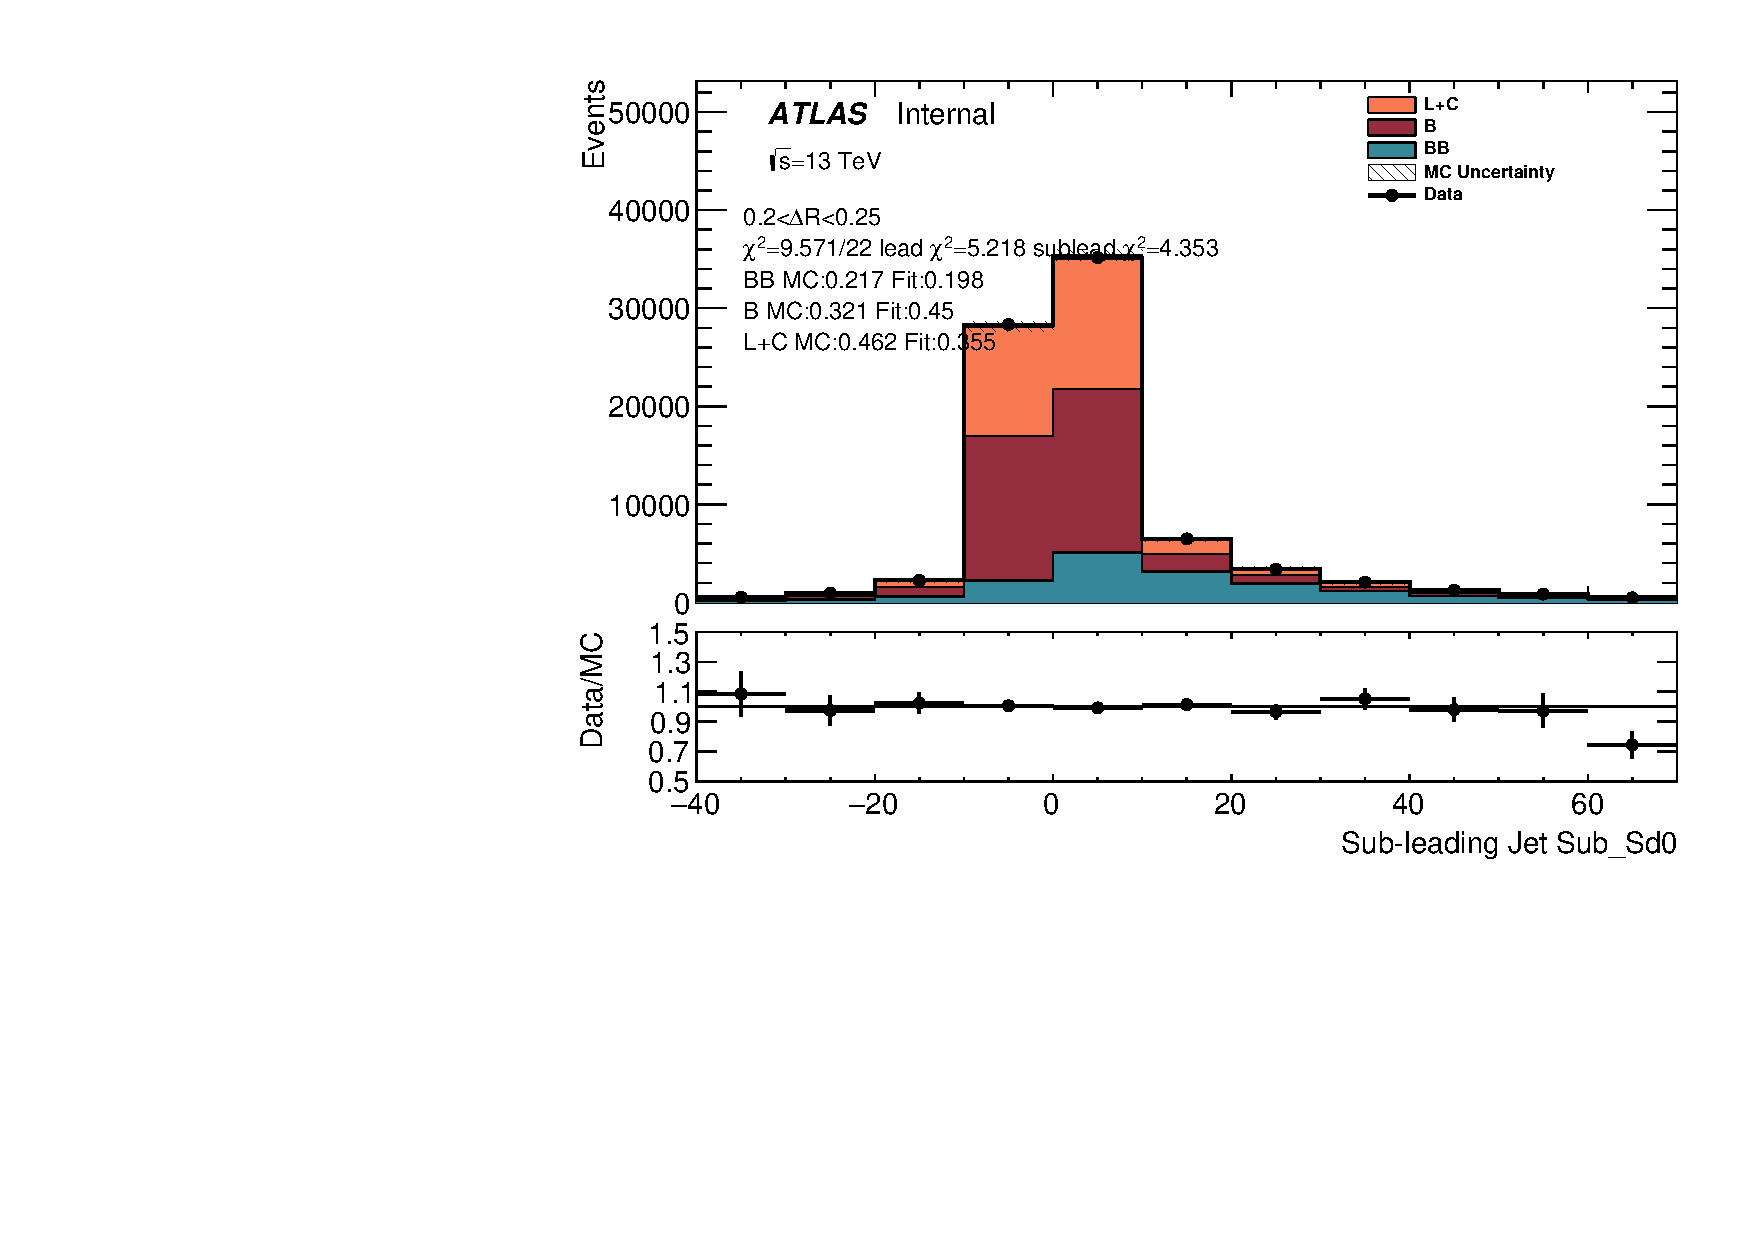
\includegraphics[width=0.32\textwidth]{figures/gbb/Sub_Sd0_Fits/Canv_Fit_02-DeltaR-025_LpT_INF_SpT_INF_coarse_y.pdf}
 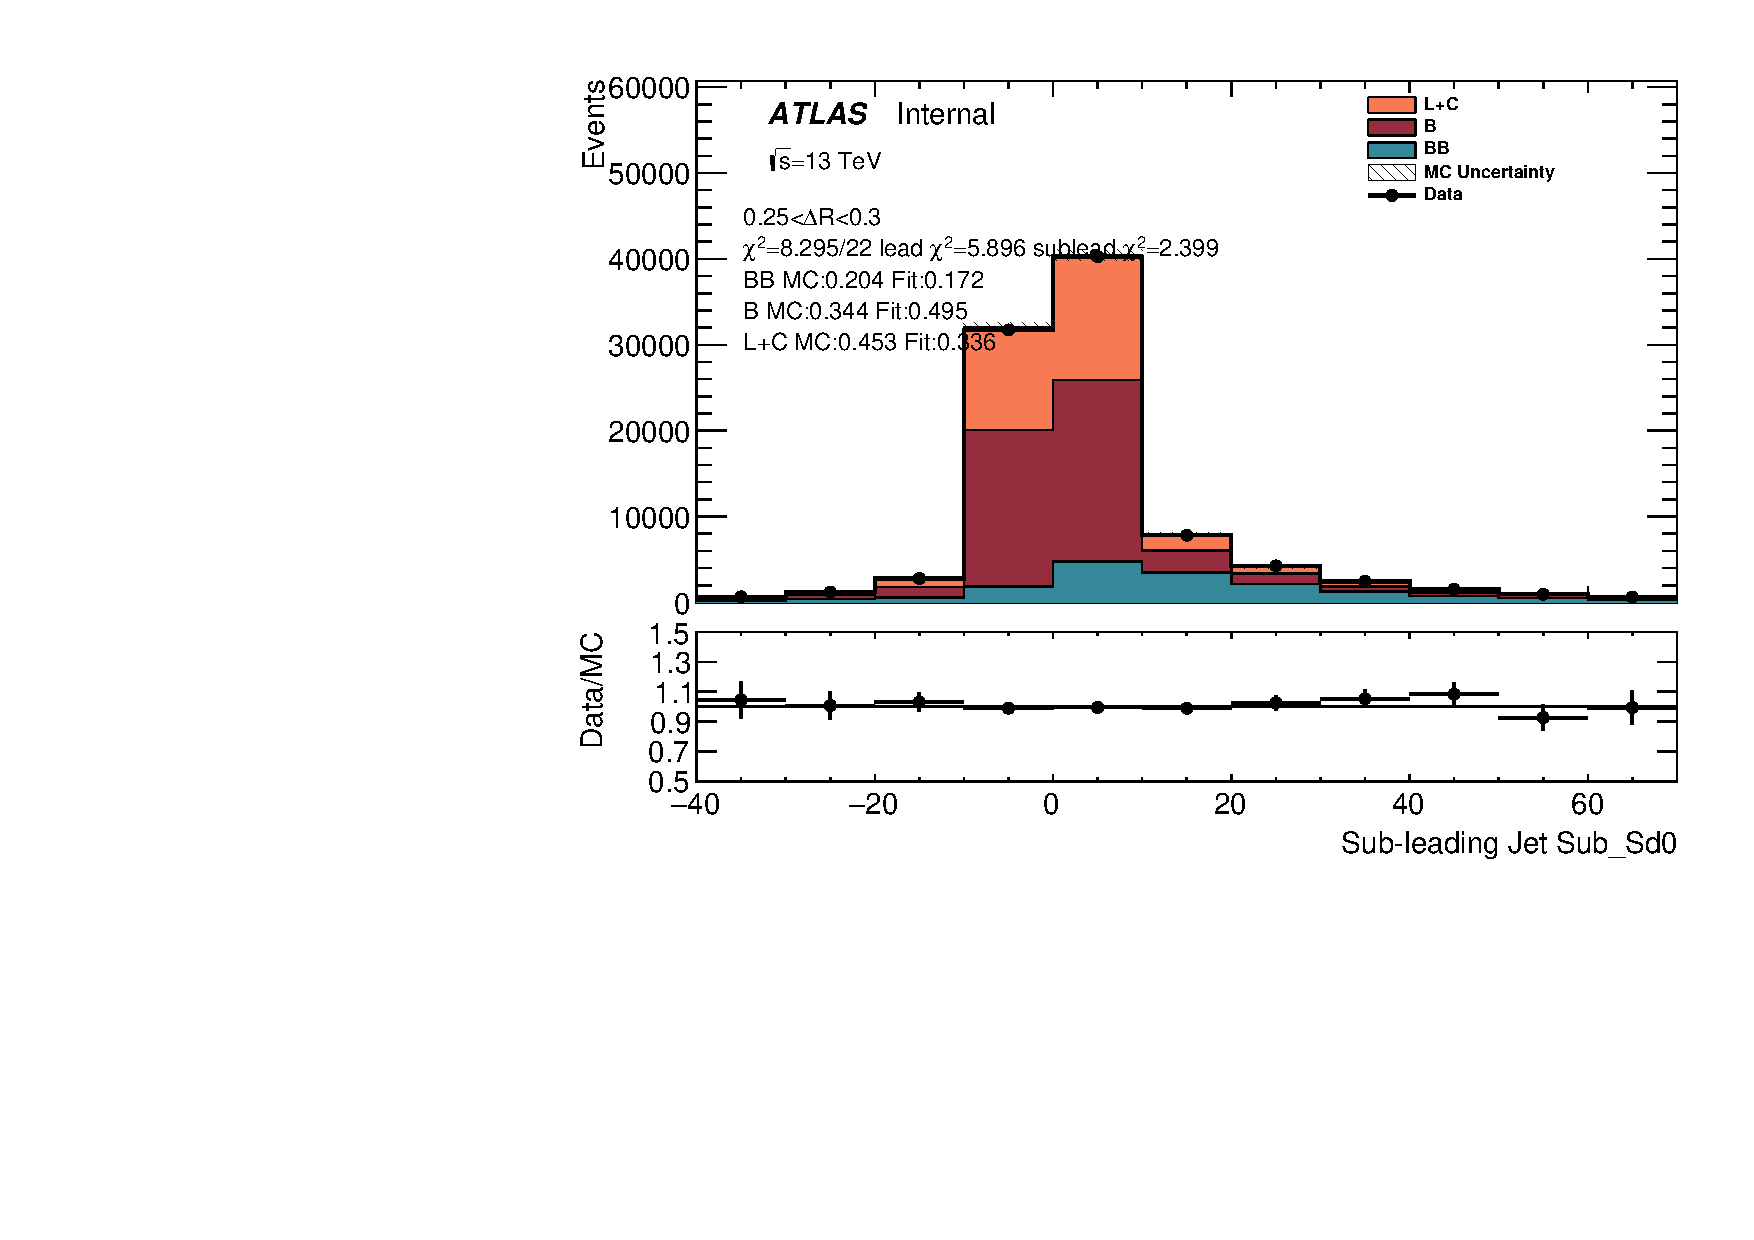
\includegraphics[width=0.32\textwidth]{figures/gbb/Sub_Sd0_Fits/Canv_Fit_025-DeltaR-03_LpT_INF_SpT_INF_coarse_y.pdf}
 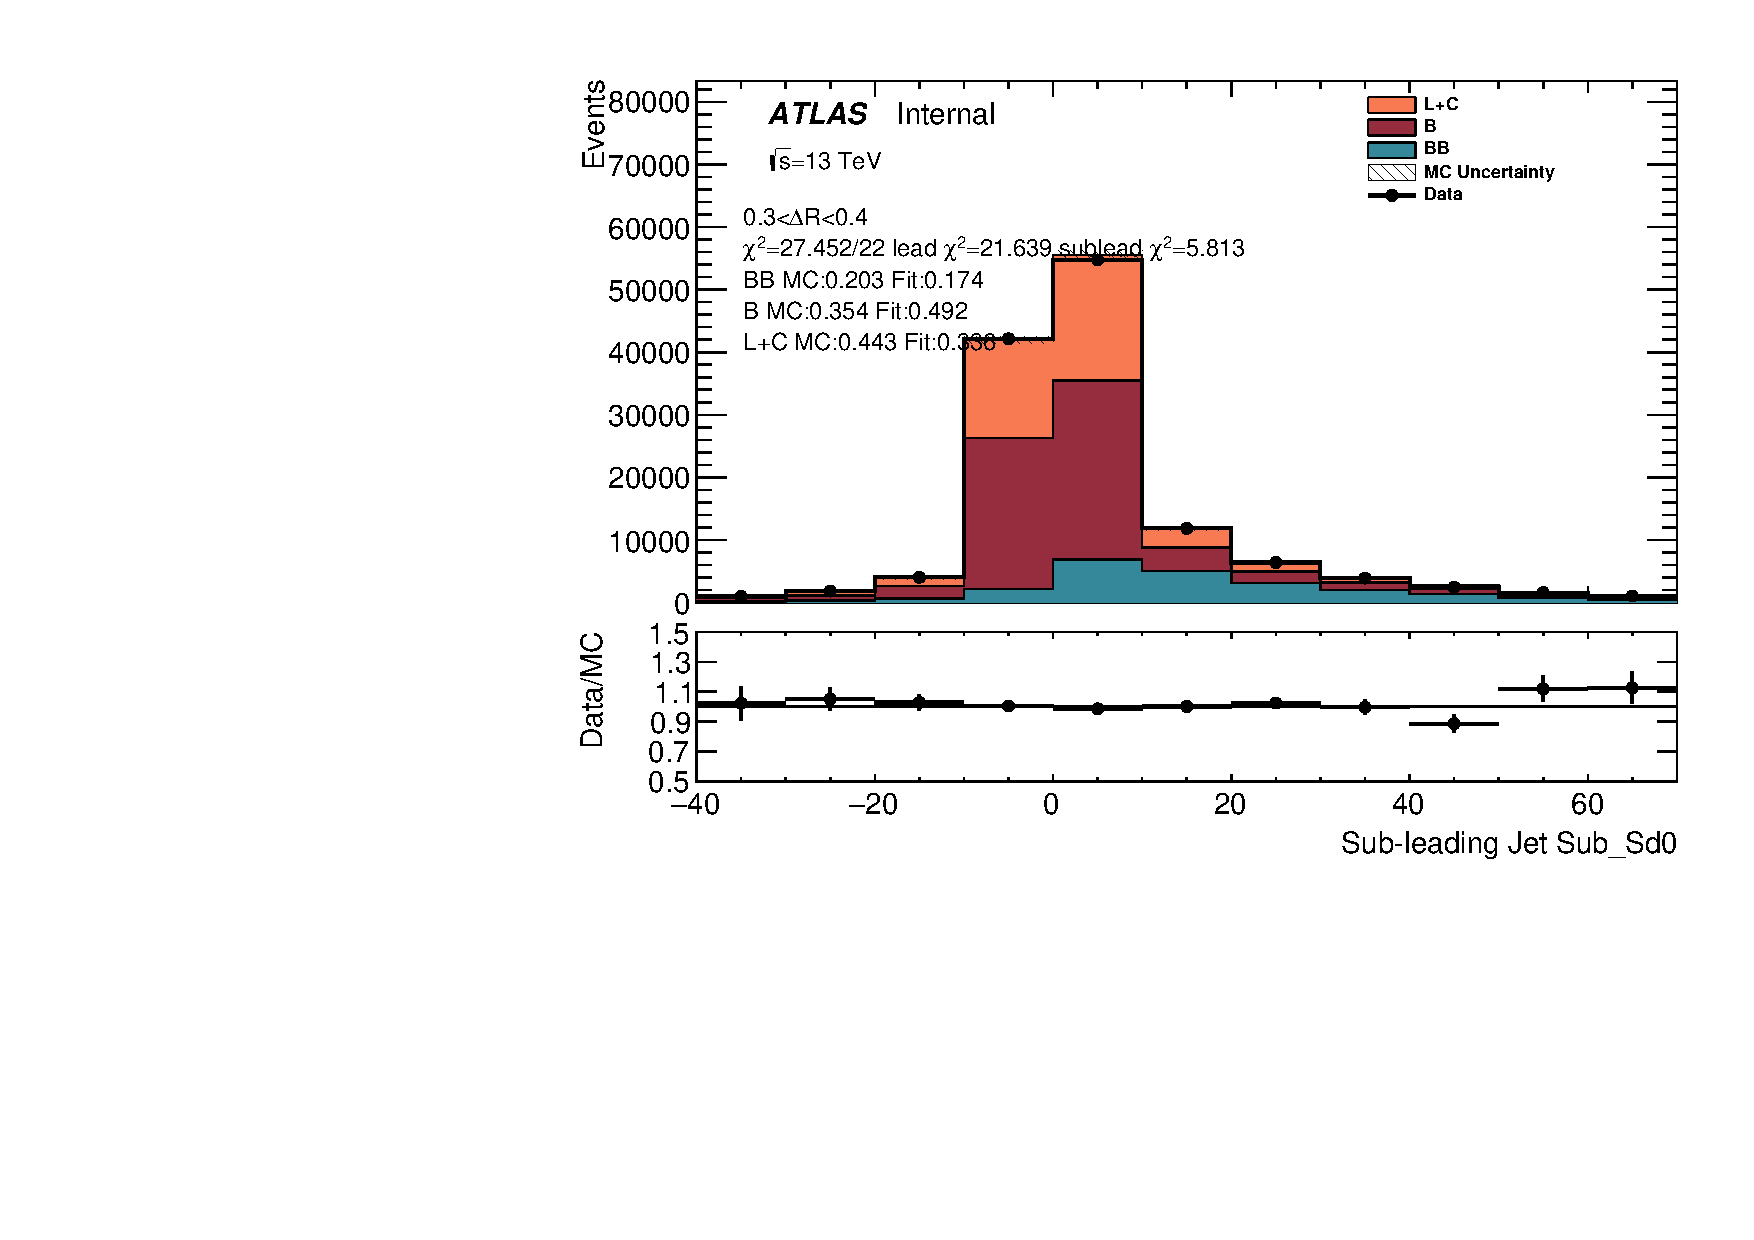
\includegraphics[width=0.32\textwidth]{figures/gbb/Sub_Sd0_Fits/Canv_Fit_03-DeltaR-04_LpT_INF_SpT_INF_coarse_y.pdf}\\
 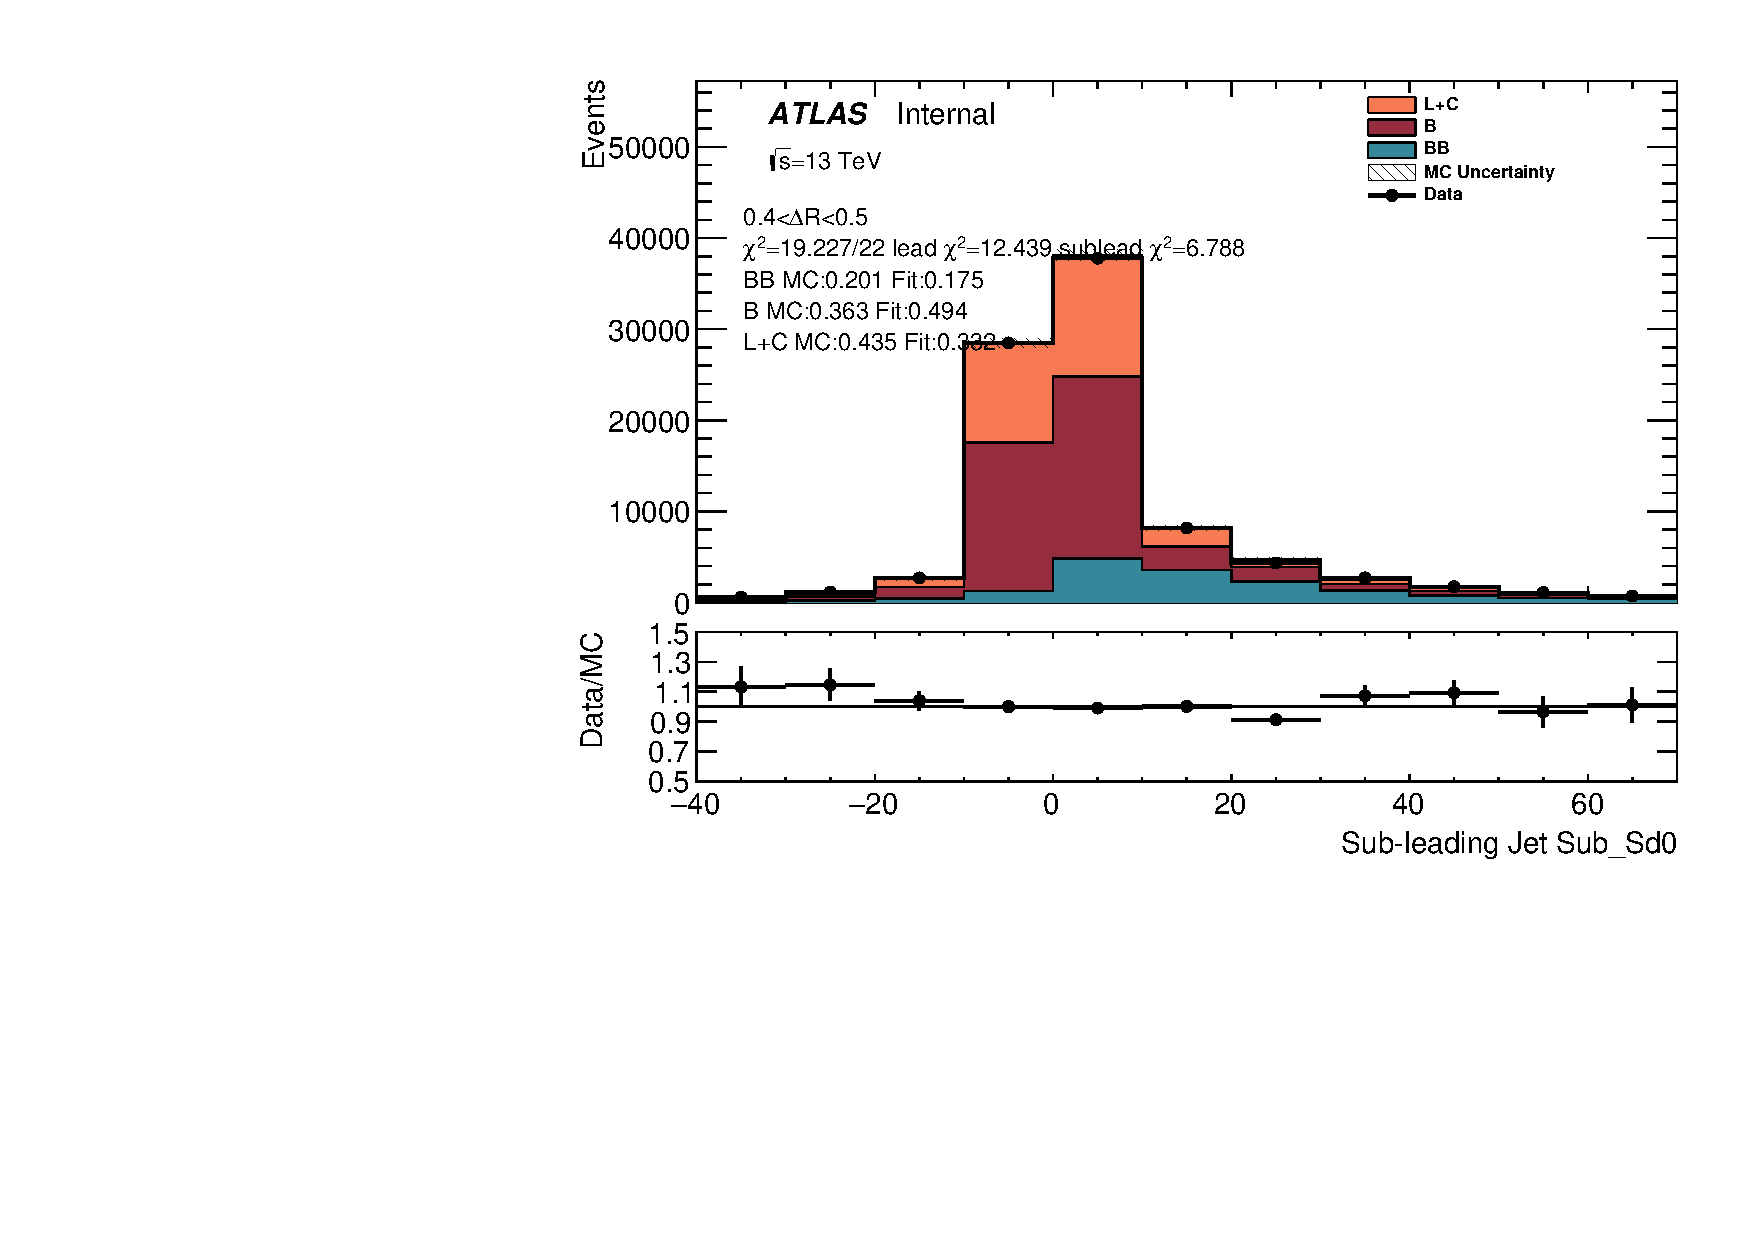
\includegraphics[width=0.32\textwidth]{figures/gbb/Sub_Sd0_Fits/Canv_Fit_04-DeltaR-05_LpT_INF_SpT_INF_coarse_y.pdf}
 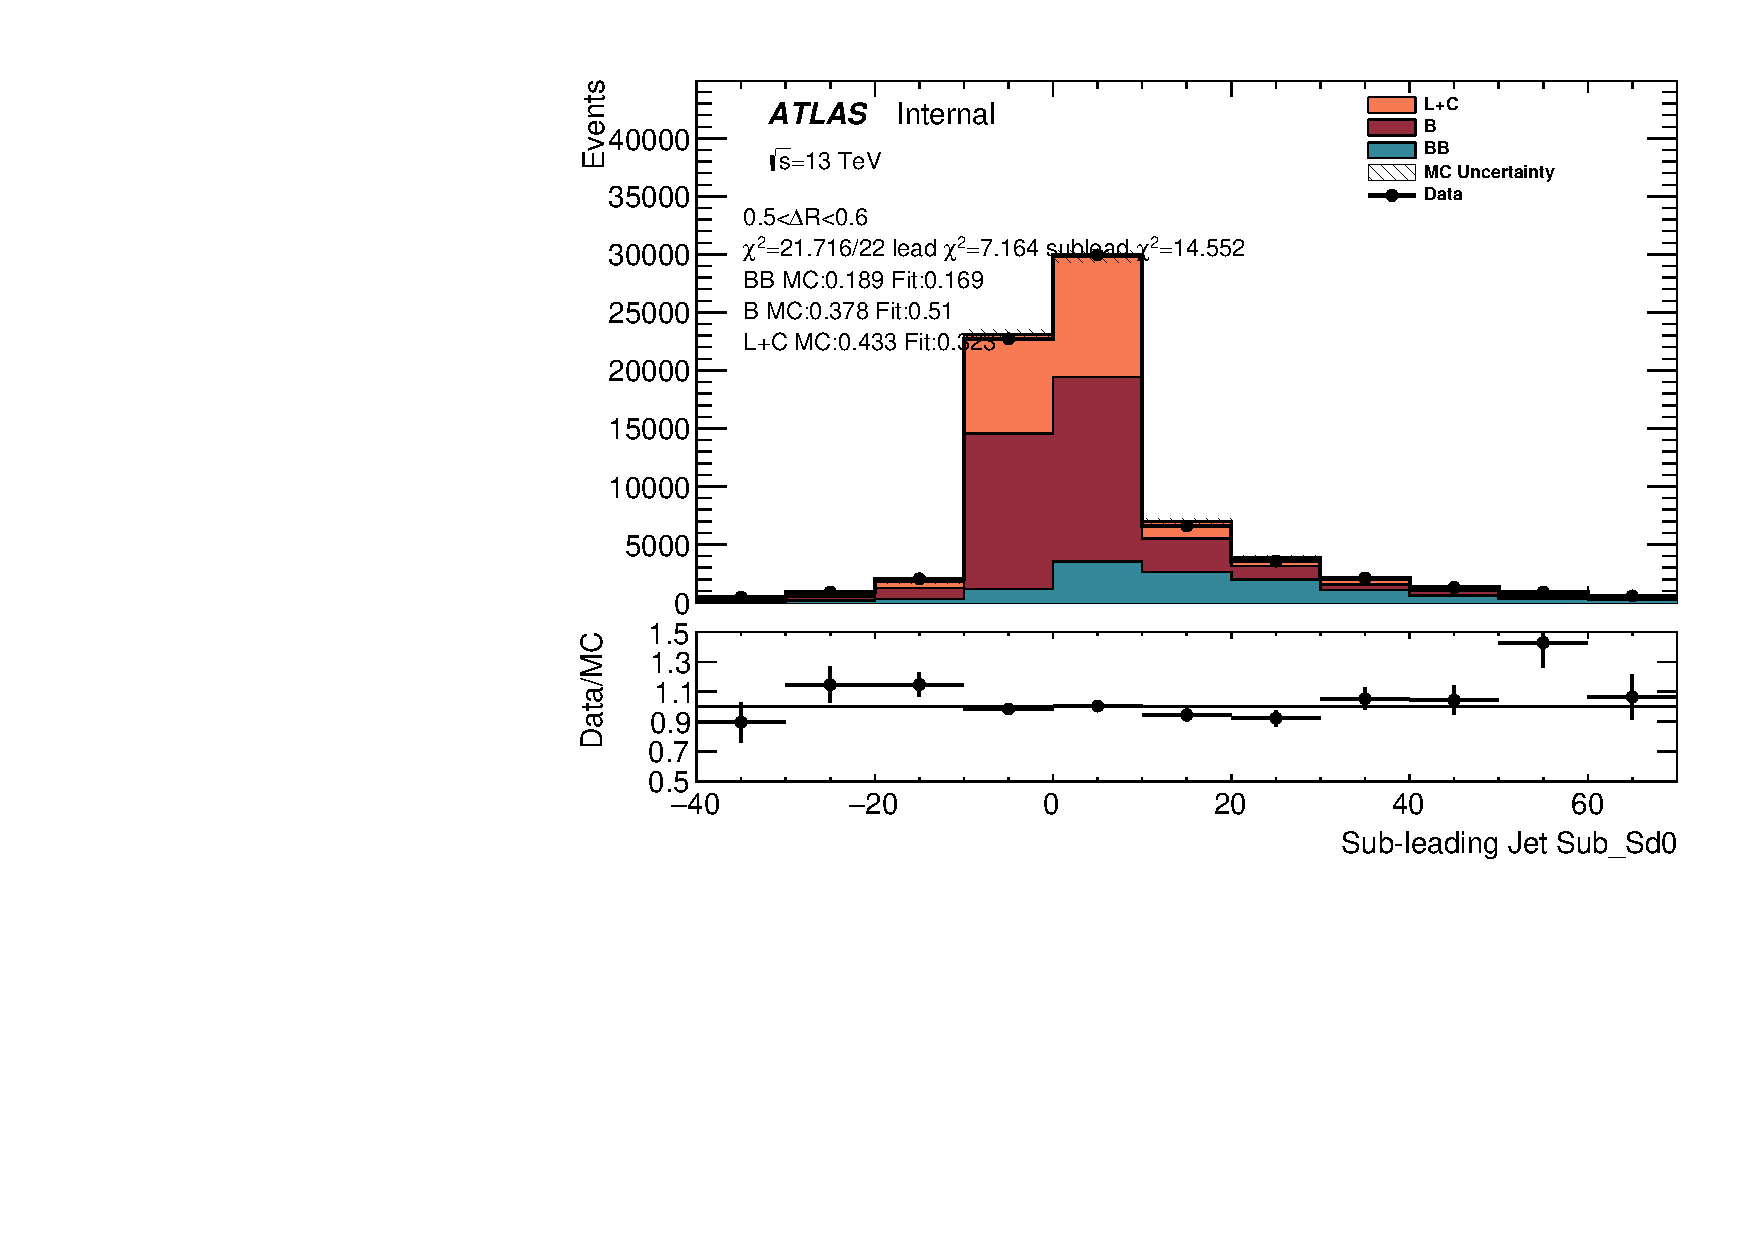
\includegraphics[width=0.32\textwidth]{figures/gbb/Sub_Sd0_Fits/Canv_Fit_05-DeltaR-06_LpT_INF_SpT_INF_coarse_y.pdf}
 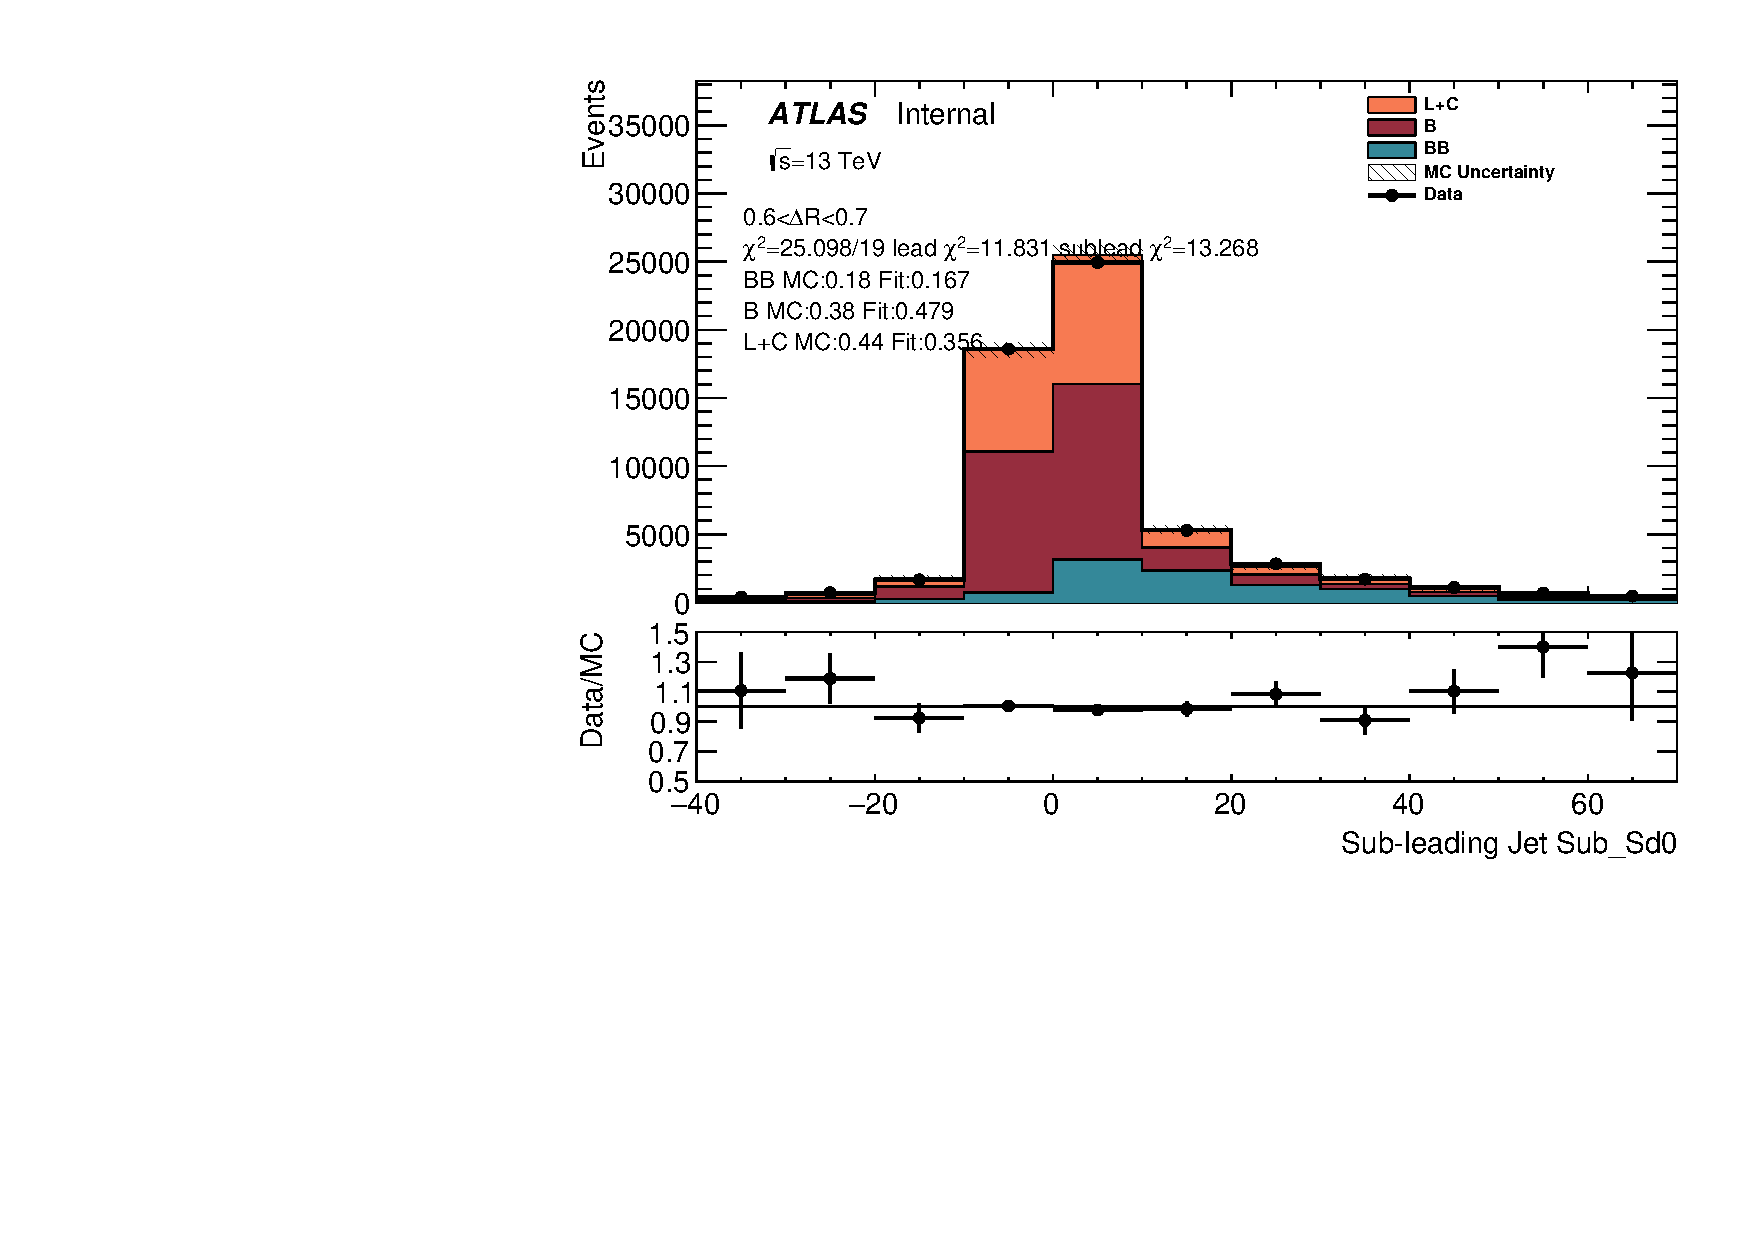
\includegraphics[width=0.32\textwidth]{figures/gbb/Sub_Sd0_Fits/Canv_Fit_06-DeltaR-07_LpT_INF_SpT_INF_coarse_y.pdf}\\

\caption{Post-fit \subsdzero distributions of the sub-leading track jet in bins of $\Delta R$. }
  \label{fig:dR-postfits-subleading}
\end{figure}


\begin{figure}[htbp]
  \centering
 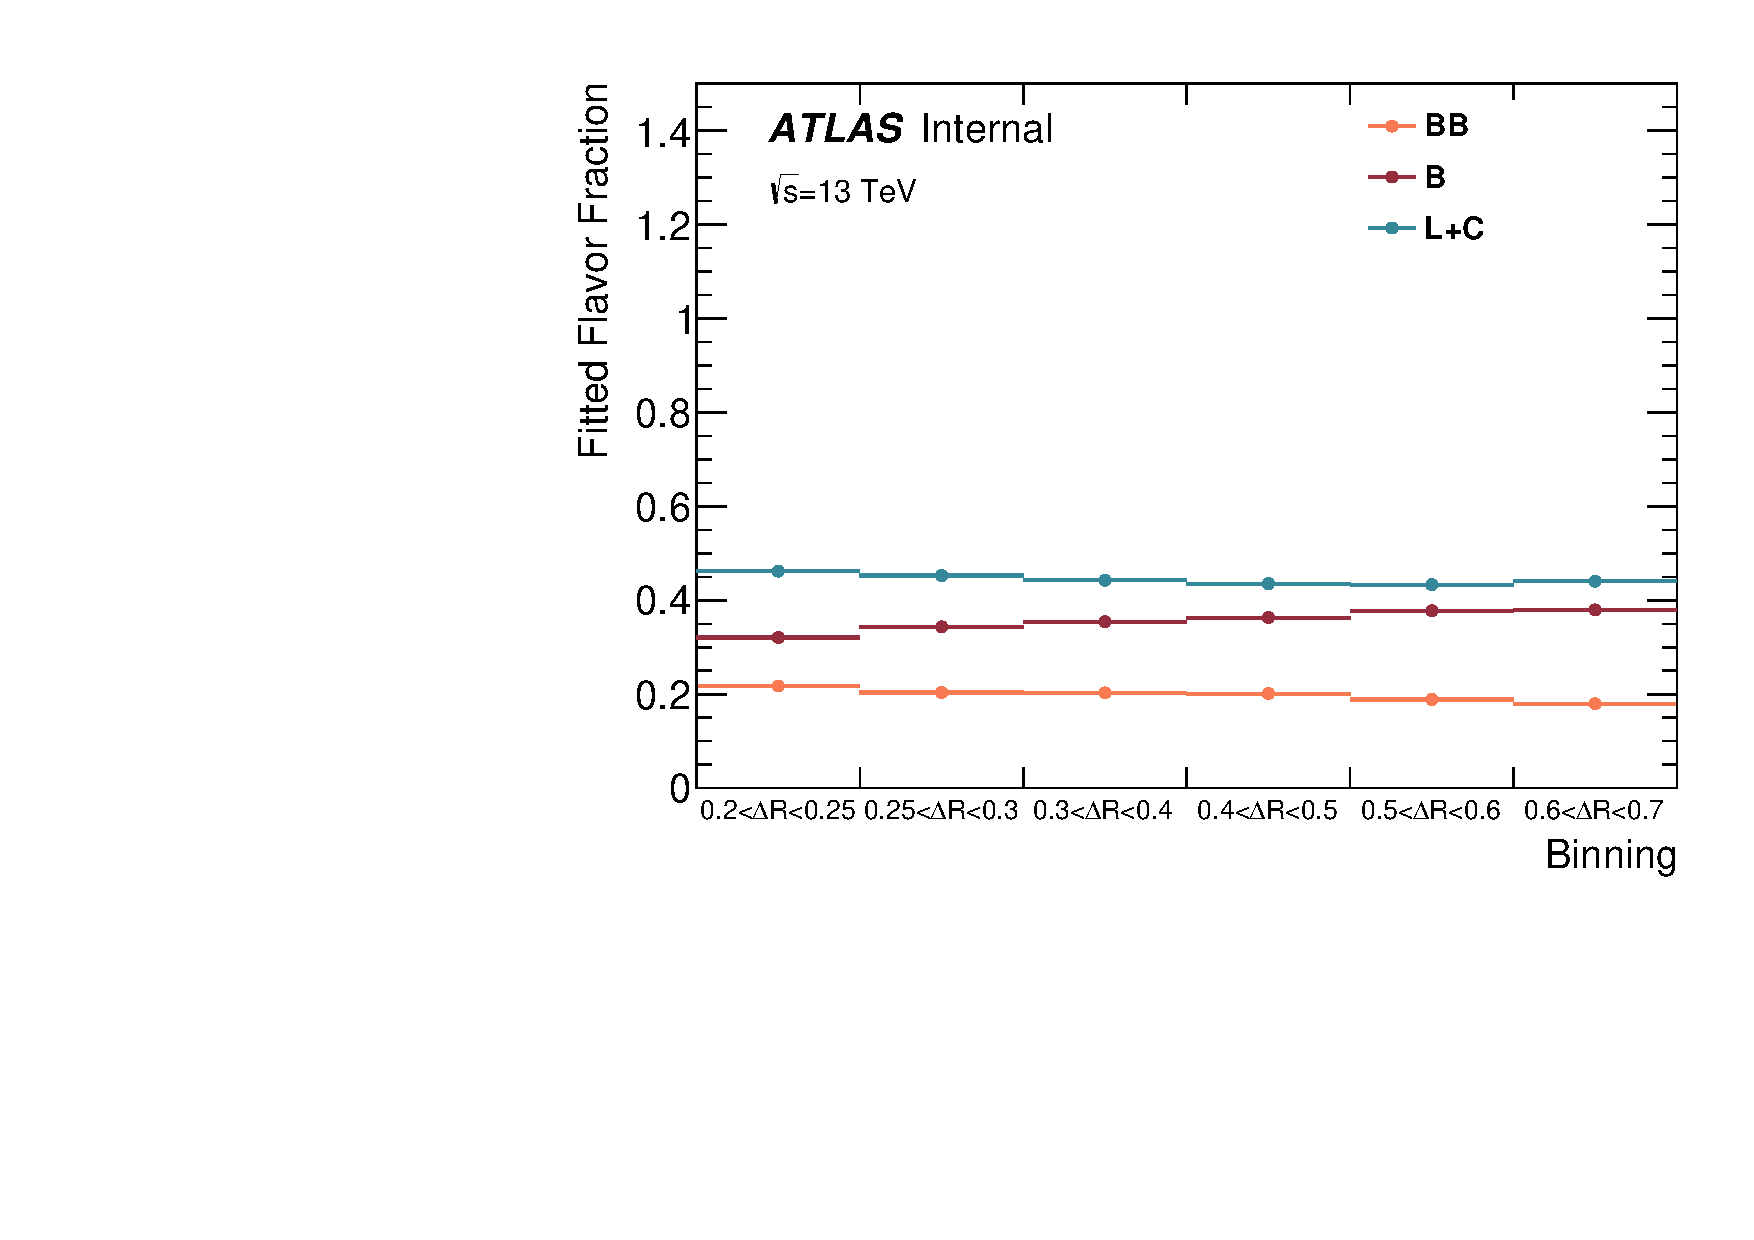
\includegraphics[width=0.45\textwidth]{figures/gbb/Sub_Sd0_Fits/Canv_dR_FitFrac_Original.pdf}
 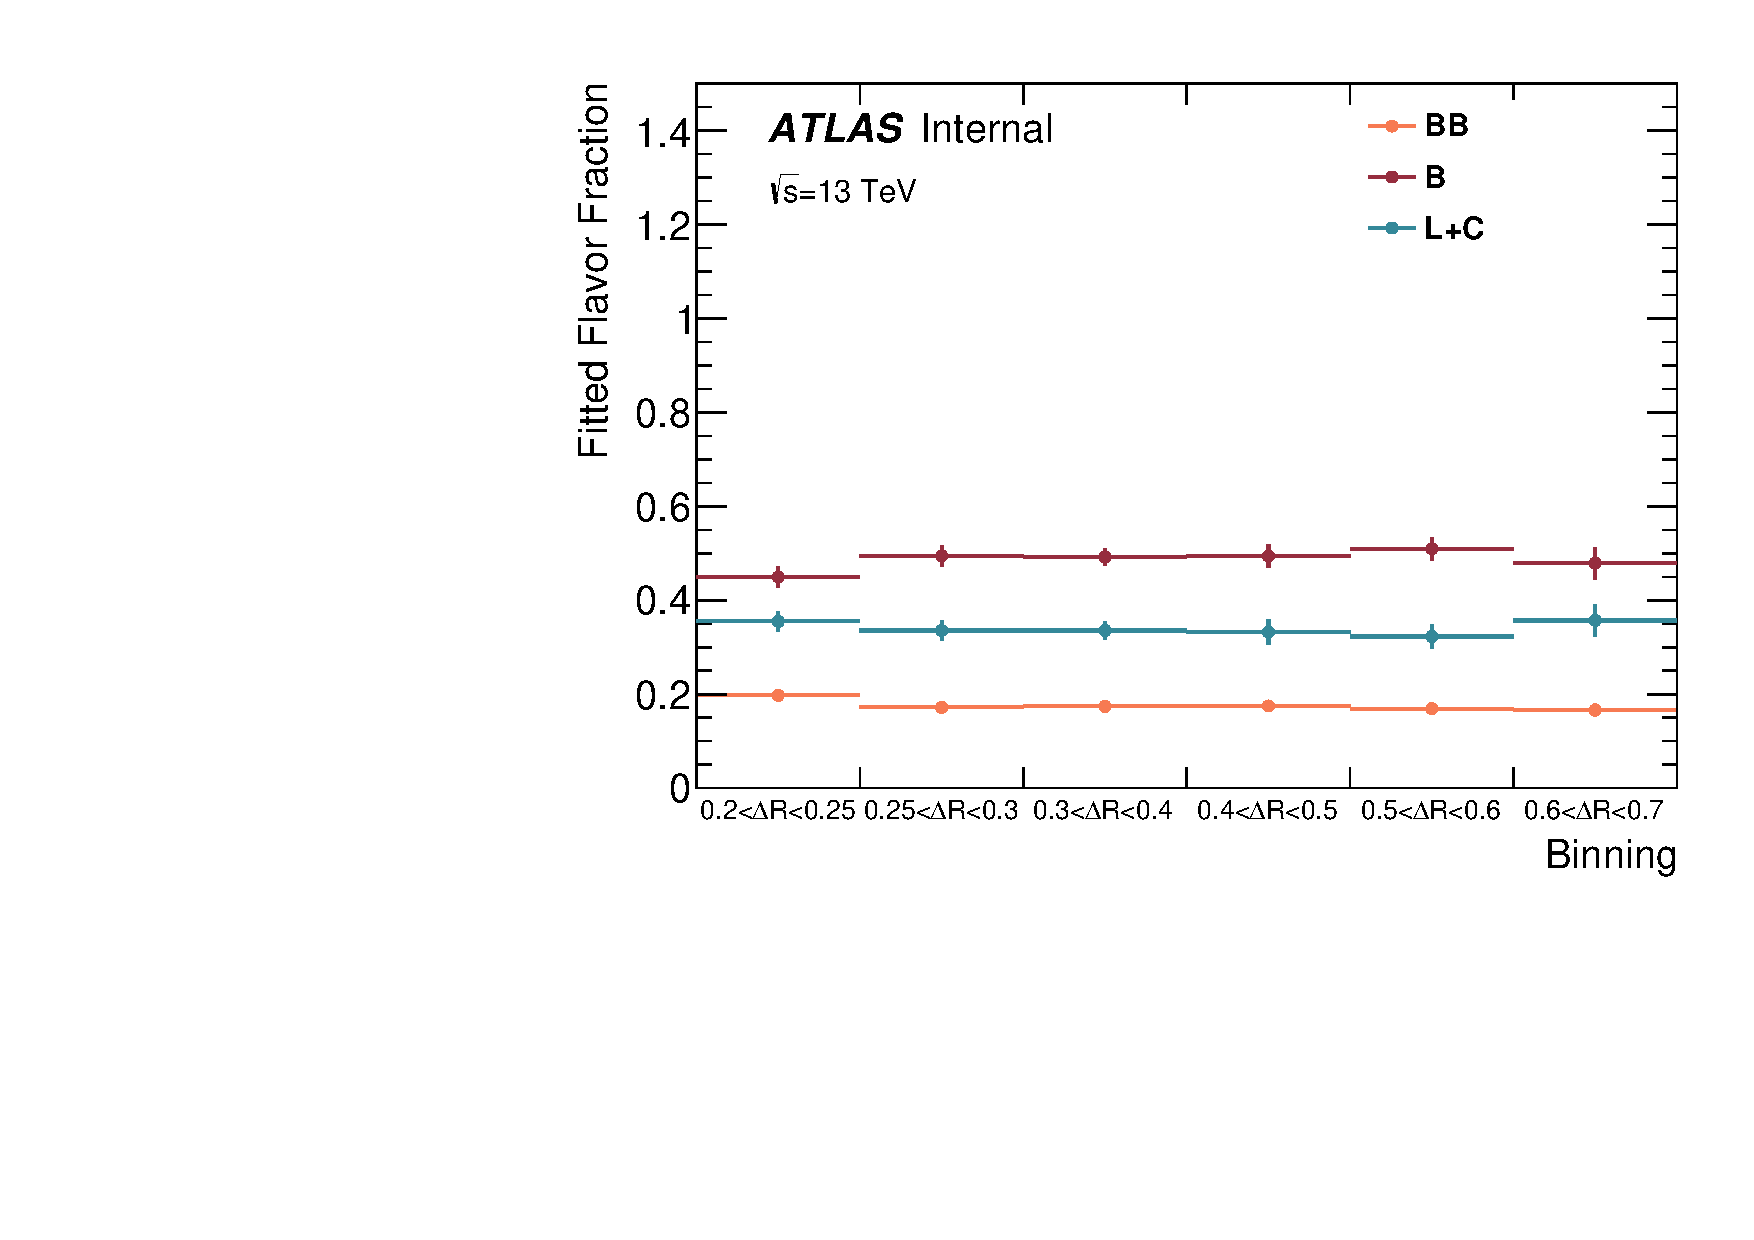
\includegraphics[width=0.45\textwidth]{figures/gbb/Sub_Sd0_Fits/Canv_dR_FitFrac_Corrected.pdf}

\caption{MC predicted (left) and fitted (right) flavor fraction in bins of $\Delta R$. The error bar is the quadrature sum of the uncertainty derived from fit range systematics and fit statistics as defined in Sec.~\ref{sec:gbb-sub_systematics}}
  \label{fig:dR-fitfrac}
\end{figure}

\begin{figure}[htbp]
  \centering
 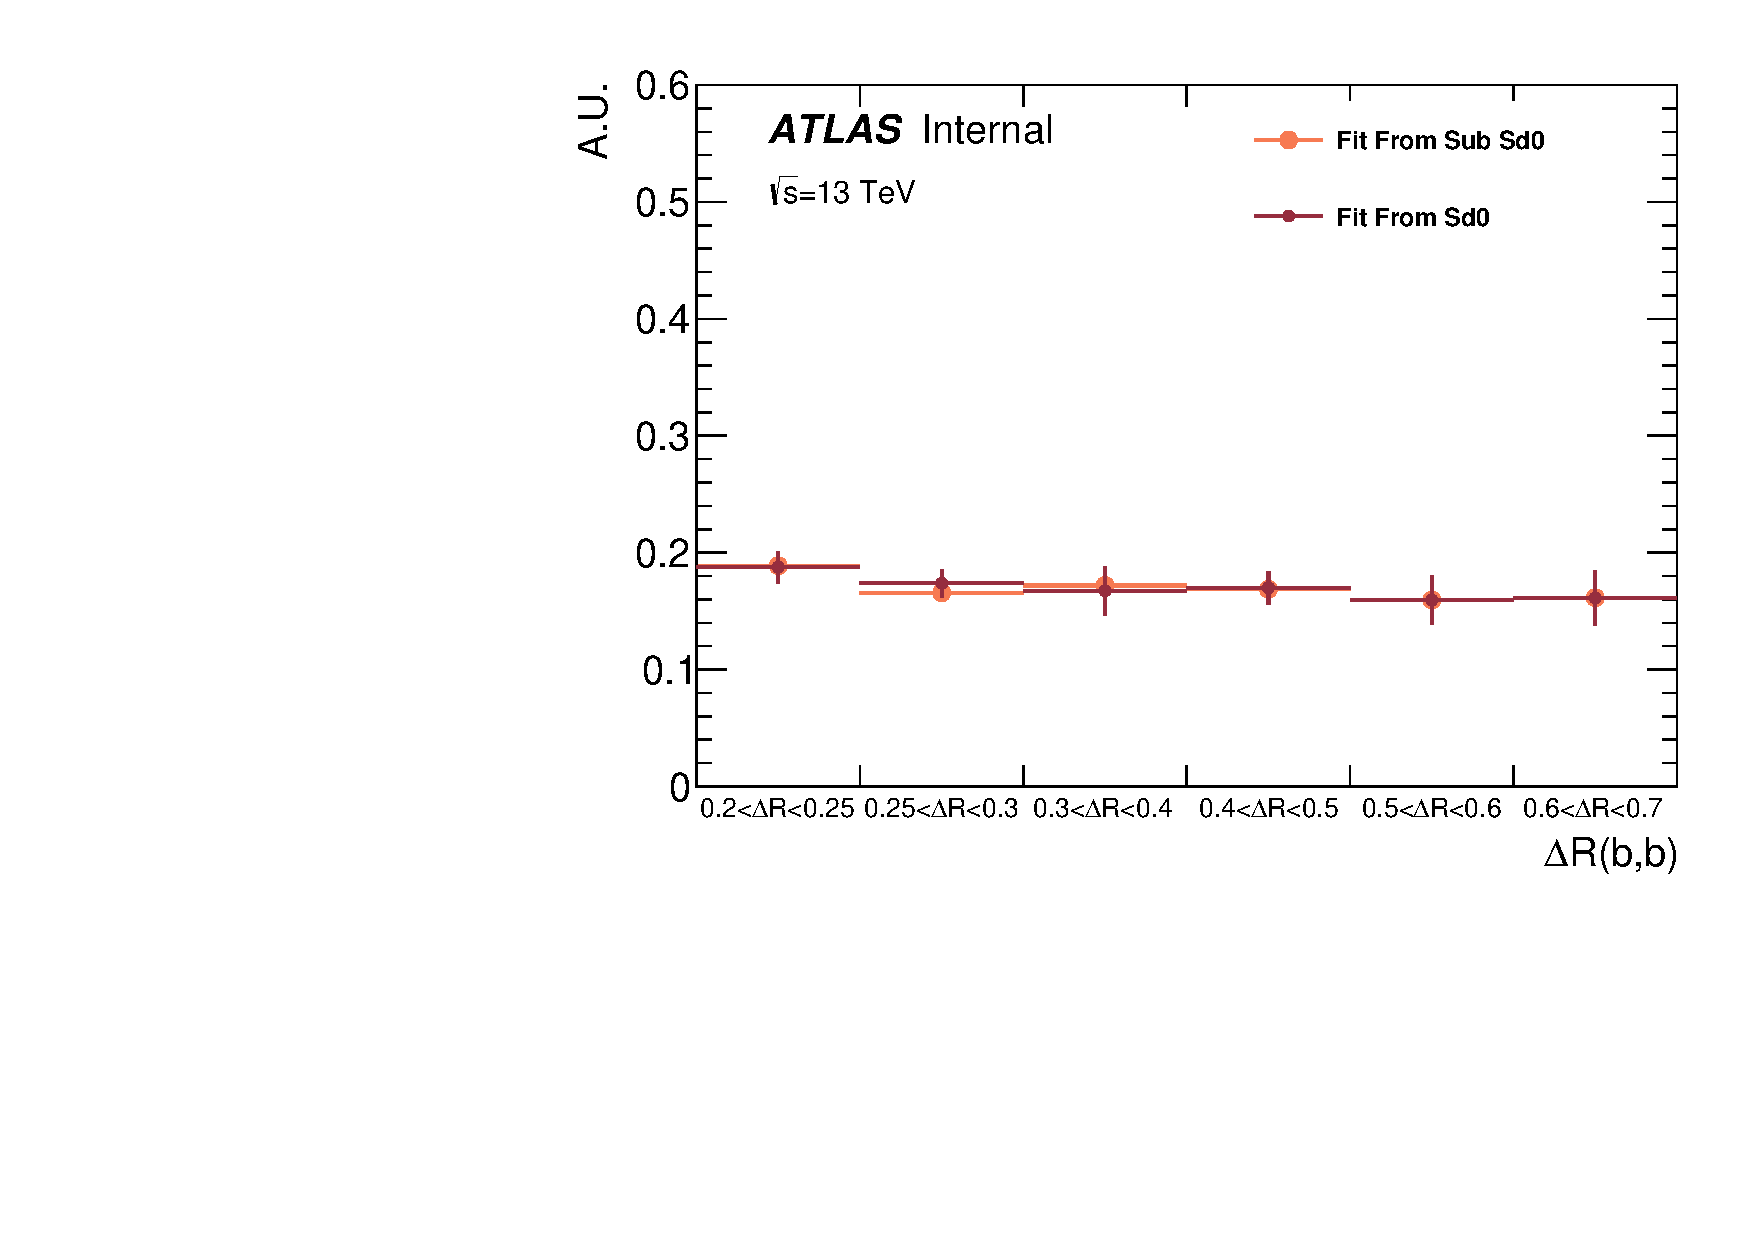
\includegraphics[width=0.45\textwidth]{figures/gbb/Sub_Sd0_Fits/Canv_dR_leadCrossCheck.pdf}
 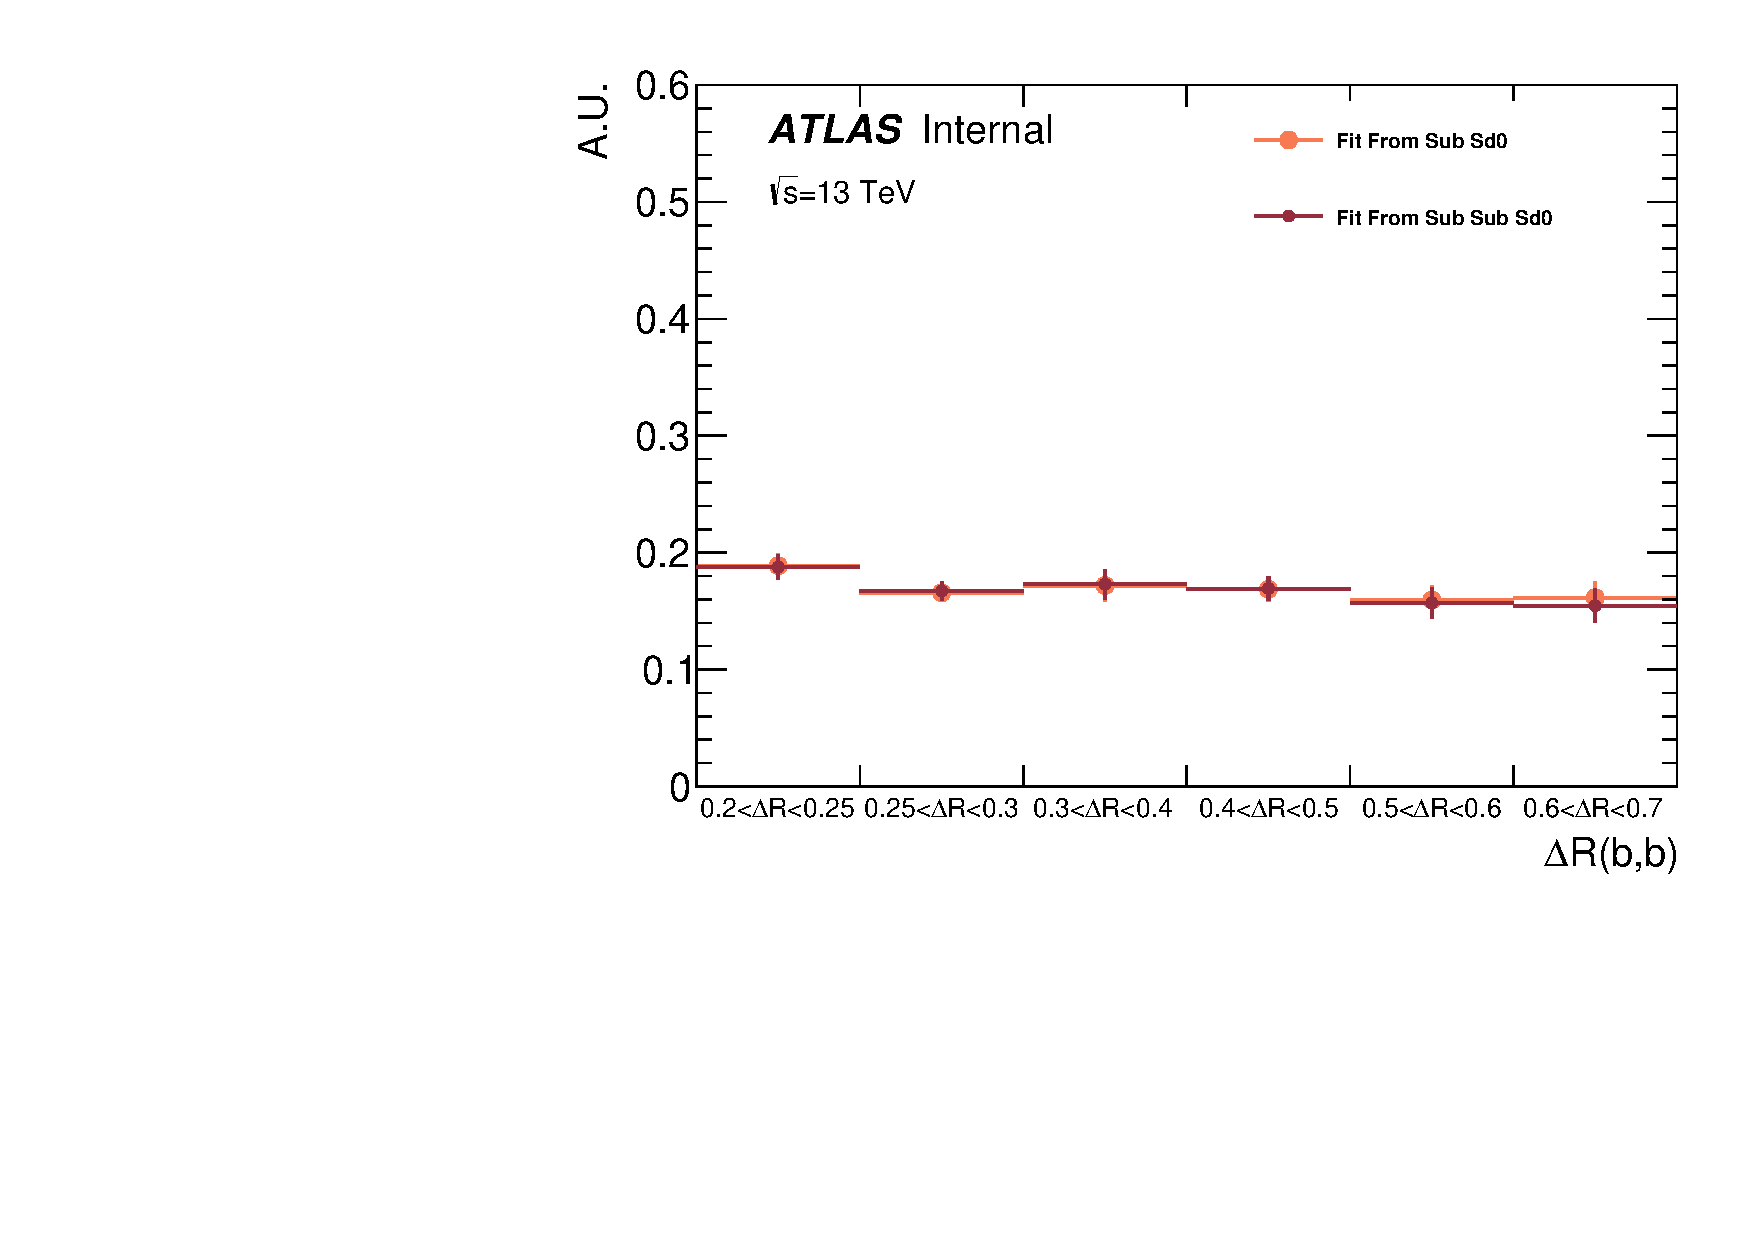
\includegraphics[width=0.45\textwidth]{figures/gbb/Sub_Sd0_Fits/Canv_dR_subsubCrossCheck.pdf}\\
 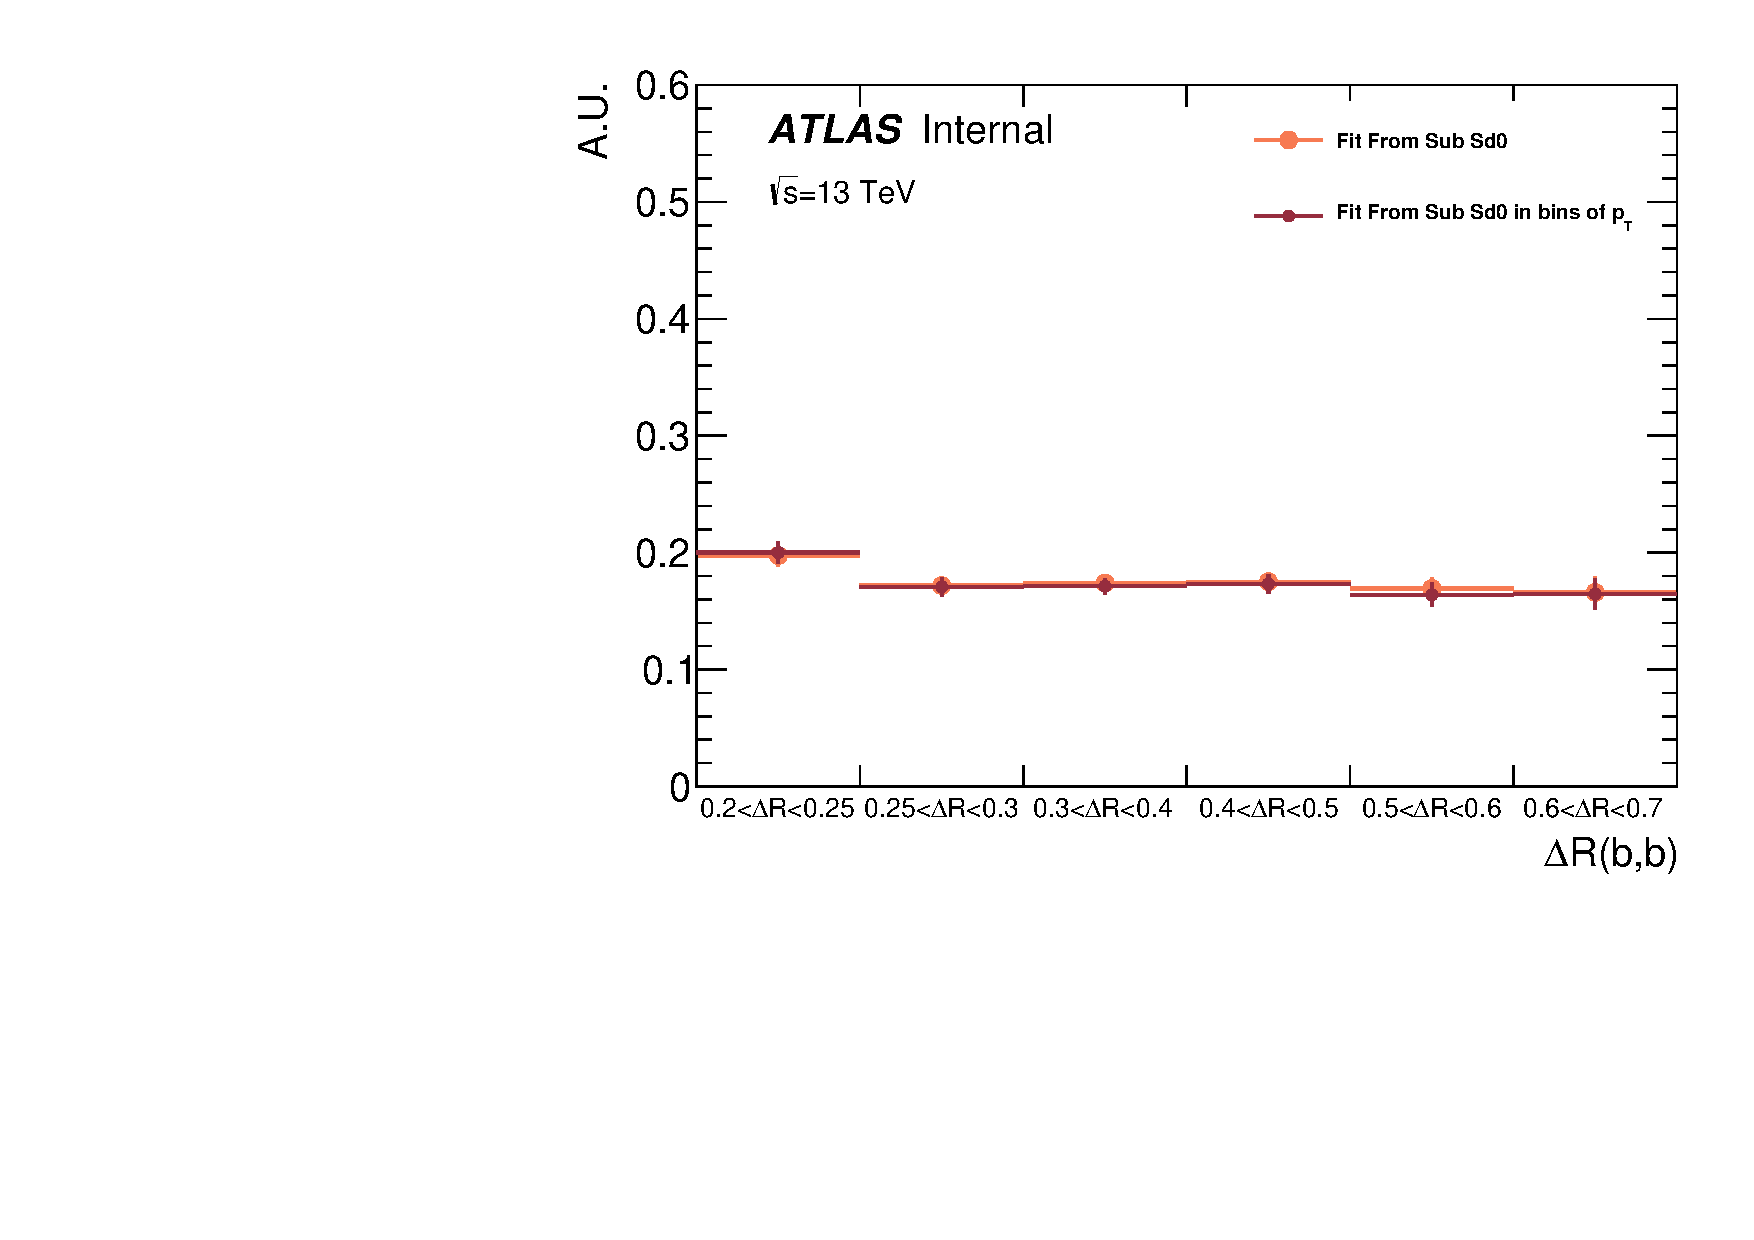
\includegraphics[width=0.45\textwidth]{figures/gbb/Sub_Sd0_Fits/Canv_dR_ptbinCrossCheck.pdf}
 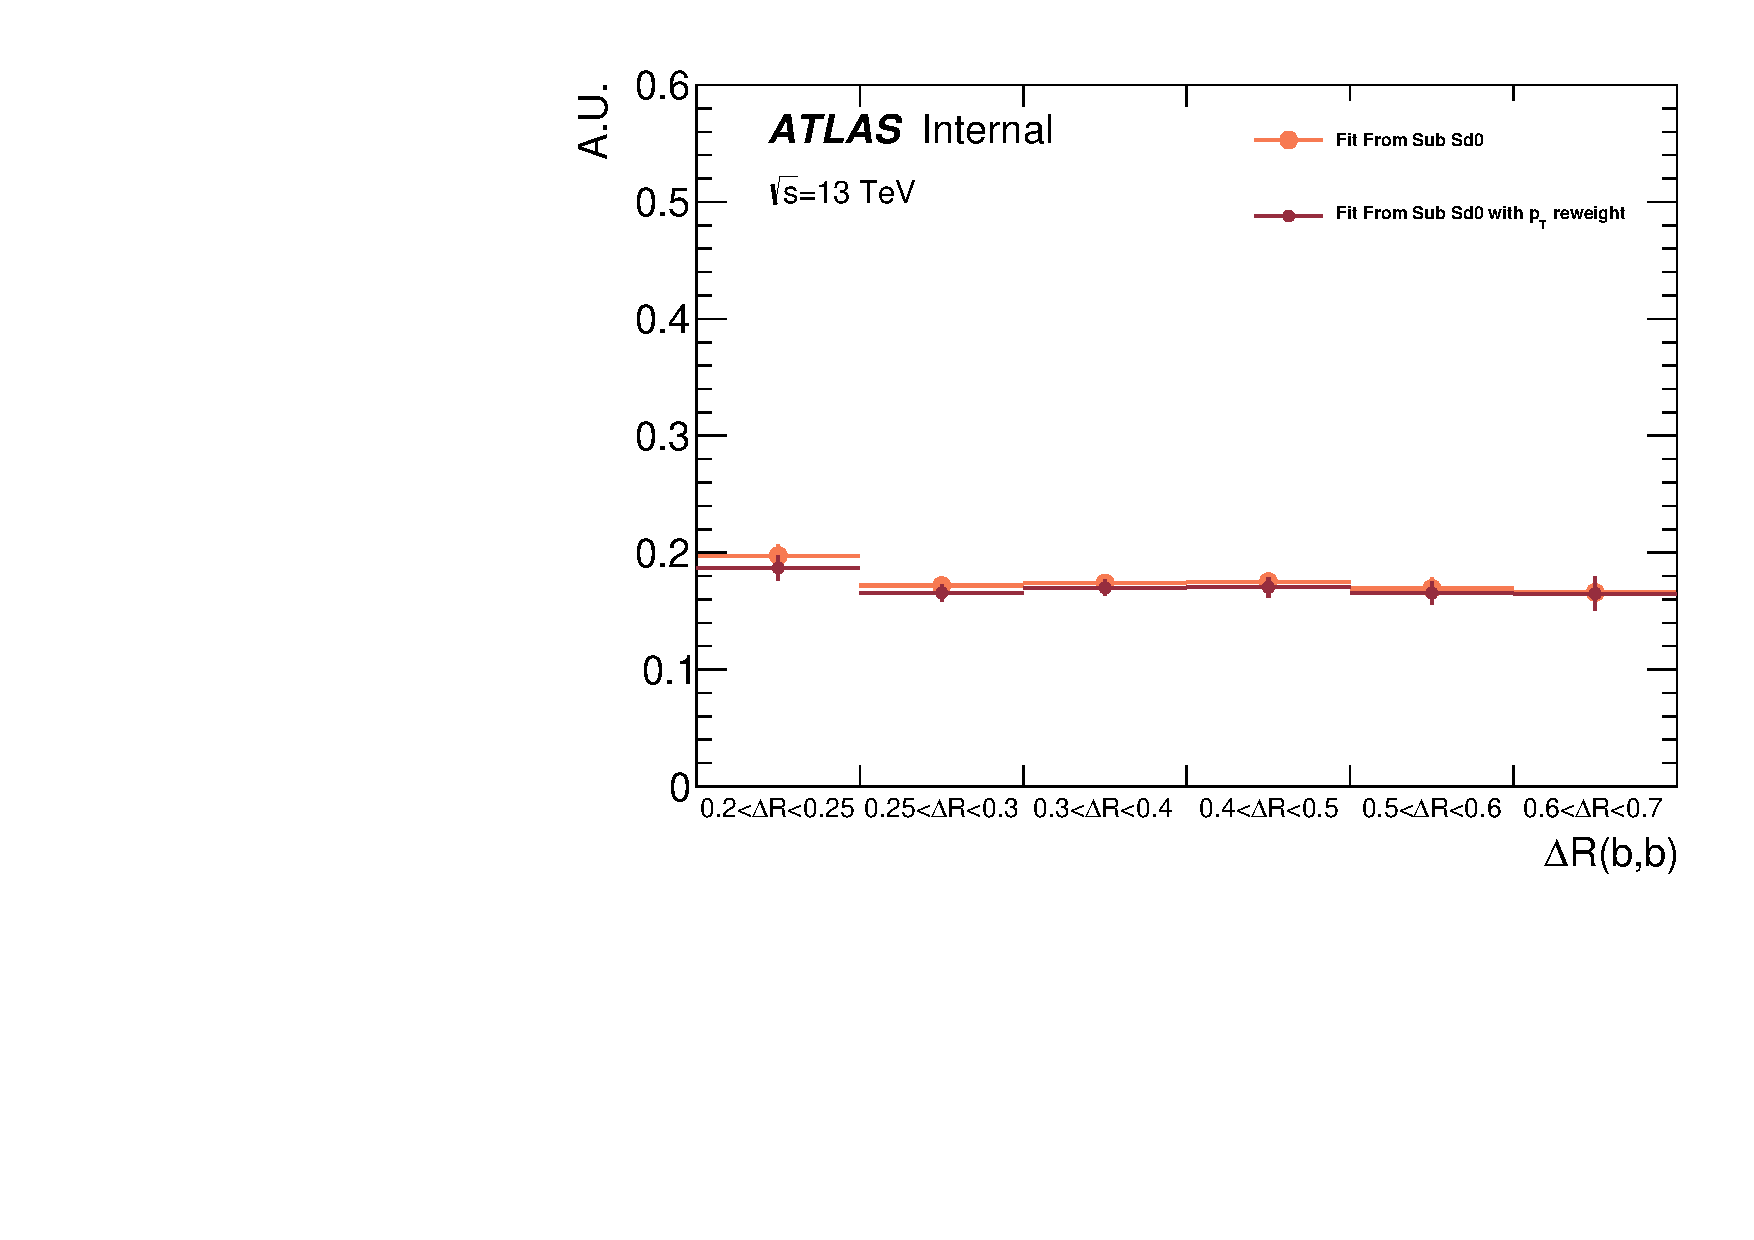
\includegraphics[width=0.45\textwidth]{figures/gbb/Sub_Sd0_Fits/Canv_dR_noreweightCrossCheck.pdf}\\
\caption{Comparison of flavor fractions fitted (1) using \subsdzero and \sdzero (top left), (2) using \subsdzero and \subsubsdzero (top right), (3) using inclusive and $p_T$ parameterized templates (bottom left) and (4) with and without track jet kinematic reweighting in bins of $\Delta R$}
  \label{fig:dR-fitfrac-crosscheck}
\end{figure}


\clearpage

\begin{table}[htbp]
\centering
\caption{Fit systematics size in percentage in bins of $\Delta R$}
\label{tab:dRsys}
\resizebox{\textwidth}{!}{
\begin{tabular}{lrrrrrr}
\hline
Syst Name                          & 0.2$<\Delta R<$0.25 & 0.25$<\Delta R<$0.3 & 0.3$<\Delta R<$0.4 & 0.4$<\Delta R<$0.5 & 0.5$<\Delta R<$0.6 & 0.6$<\Delta R<$0.7 \\ \hline
Trk\_Eff                           & 0.46               & 8.58                 & 2.6                  & 5.63                 & -0.67                \\
Trk\_Fake                          & -1.28              & 3.84                 & 9.64                 & 5.93                 & 3.64                 \\
Trk\_In\_Jet                       & -0.67              & 5.78                 & 9.2                  & 5.98                 & -2.07                \\
Trk\_Sagitta                       & -1.73              & 3.2                  & 2.64                 & 1.08                 & -1.95                \\
Trk\_d0Smear                       & -0.9               & 8.5                  & 3.19                 & 8.35                 & -3.76                \\
FitRange\_Left                     & 0.35               & 1.02                 & -0.18                & 0.16                 & -0.06                \\
FitRange\_Right                    & 1.0                & 0.19                 & -0.55                & -1.84                & -0.29                \\
BLUp                               & 2.42               & 1.93                 & 2.8                  & 2.74                 & 1.65                 \\
BLDn                               & -4.01              & -2.81                & -4.87                & -4.89                & -2.78                \\
BCUp                               & -3.82              & -2.94                & -4.76                & -4.75                & -2.75                \\
BCDn                               & 2.39               & 2.0                  & 2.67                 & 2.87                 & 1.56                 \\
LLUp                               & 3.96               & 3.49                 & 4.31                 & 4.71                 & 3.05                 \\
LLDn                               & -2.57              & -1.77                & -2.92                & -3.05                & -1.81                \\
LCUp                               & -0.88              & -0.49                & -0.99                & -0.94                & -0.14                \\
LCDn                               & 0.83               & 0.8                  & 0.66                 & 0.65                 & 0.26                 \\
LBUp                               & -1.26              & -0.94                & -1.06                & -1.64                & -1.27                \\
LBDn                               & 0.97               & 0.63                 & 0.51                 & 0.78                 & 0.51                 \\
CLUp                               & 4.46               & 4.85                 & 3.11                 & 3.99                 & 3.67                 \\
CLDn                               & -3.5               & -4.28                & -2.53                & -3.29                & -2.87                \\
CCUp                               & -4.99              & -5.77                & -4.81                & -6.23                & -4.69                \\
CCDn                               & 3.43               & 4.22                 & 3.35                 & 4.28                 & 3.33                 \\
CBUp                               & -2.16              & -1.24                & -1.61                & -1.26                & -1.54                \\
CBDn                               & 0.98               & 1.03                 & 0.55                 & 0.52                 & 0.77                 \\
StatUp                             & 4.0                & 4.83                 & 4.49                 & 4.44                 & 4.3                  \\
StatDn                             & -4.2               & -4.63                & -4.29                & -4.51                & -3.87                \\
FT\_EFF\_Eigen\_B\_0\_\_1down      & 0.17               & 0.26                 & 0.07                 & 0.22                 & 0.1                  \\
FT\_EFF\_Eigen\_B\_1\_\_1down      & -0.16              & 0.07                 & -0.21                & -0.04                & -0.21                \\
FT\_EFF\_Eigen\_C\_0\_\_1down      & -0.29              & -0.13                & -0.41                & -0.35                & -0.04                \\
FT\_EFF\_Eigen\_C\_1\_\_1down      & -0.42              & -0.22                & -0.71                & -0.73                & -0.54                \\
FT\_EFF\_Eigen\_C\_2\_\_1down      & -0.35              & 0.09                 & -0.5                 & -0.57                & 0.13                 \\
FT\_EFF\_Eigen\_Light\_0\_\_1down  & 1.97               & 1.68                 & 1.93                 & 2.23                 & 1.74                 \\
FT\_EFF\_Eigen\_Light\_1\_\_1down  & 1.54               & 1.15                 & 1.66                 & 1.87                 & 1.25                 \\
FT\_EFF\_Eigen\_Light\_2\_\_1down  & 1.86               & 1.68                 & 1.21                 & 1.4                  & 1.33                 \\
FT\_EFF\_Eigen\_Light\_3\_\_1down  & -0.12              & 0.36                 & -0.02                & -0.18                & 0.07                 \\
FT\_EFF\_extrapolation\_\_1down    & -0.93              & -0.92                & -0.62                & -0.43                & -0.71                \\
FT\_EFF\_Eigen\_B\_0\_\_1up        & 0.06               & 0.3                  & 0.18                 & -0.17                & 0.03                 \\
FT\_EFF\_Eigen\_B\_1\_\_1up        & 0.35               & 0.28                 & 0.22                 & 0.16                 & 0.1                  \\
FT\_EFF\_Eigen\_C\_0\_\_1up        & 0.39               & 0.17                 & 0.3                  & 0.57                 & 0.29                 \\
FT\_EFF\_Eigen\_C\_1\_\_1up        & 1.02               & 0.44                 & 1.0                  & 1.05                 & 0.69                 \\
FT\_EFF\_Eigen\_C\_2\_\_1up        & 0.27               & 0.26                 & 0.39                 & 0.55                 & 0.39                 \\
FT\_EFF\_Eigen\_Light\_0\_\_1up    & -2.39              & -1.81                & -2.45                & -3.63                & -1.78                \\
FT\_EFF\_Eigen\_Light\_1\_\_1up    & -1.56              & -0.93                & -1.77                & -2.25                & -1.38                \\
FT\_EFF\_Eigen\_Light\_2\_\_1up    & -2.06              & -1.82                & -1.21                & -1.46                & -1.29                \\
FT\_EFF\_Eigen\_Light\_3\_\_1up    & -0.01              & -0.11                & -0.12                & 0.48                 & -0.06                \\
FT\_EFF\_extrapolation\_\_1up      & 1.02               & 0.78                 & 0.39                 & 0.25                 & 0.77                 \\
JET\_JER                           & 0.05               & 6.45                 & 3.34                 & 2.48                 & -1.94                \\
JET\_Comb\_Baseline\_All\_\_1up    & 3.31               & 12.12                & 7.8                  & 13.27                & 2.89                 \\
JET\_Comb\_Modelling\_All\_\_1down & -10.82             & -11.16               & -11.74               & -3.48                & -15.9                \\
JET\_Comb\_Modelling\_All\_\_1up   & 12.41              & 19.56                & 19.19                & 15.06                & 6.25                 \\
JET\_Comb\_TotalStat\_All\_\_1down & 0.81               & 7.21                 & 5.52                 & 5.06                 & -0.65                \\
JET\_Comb\_TotalStat\_All\_\_1up   & -2.85              & 3.38                 & 8.91                 & 6.43                 & 1.02                 \\
JET\_Comb\_Tracking\_All\_\_1down  & -1.57              & 5.69                 & 3.94                 & 3.76                 & -0.9                 \\
JET\_Comb\_Tracking\_All\_\_1up    & 3.8                & 6.89                 & 6.85                 & 9.34                 & -4.82                \\
JET\_Comb\_Baseline\_All\_\_1down  & -2.15              & -1.04                & -4.0                 & -1.58                & -7.59                \\
Sherpa                             & -9.44              & 7.11                 & 18.0                 & -16.63               & 7.05                 \\
\end{tabular}}
\end{table}



\clearpage
\subsection{\zpt}

In total, there are five bins of the \zpt observable we are measuring. The flavor fraction fits are performed for \zpt $\in\{[0, 0.1], [0.1, 0.2], [0.2, 0.3], [0.3,0.4], [0.4,0.5]\}$. The pre-fit and post-fit Data/MC comparison are shown in Figures.~\ref{fig:ZpT-prefits-leading},\ref{fig:ZpT-prefits-subleading},\ref{fig:ZpT-postfits-leading},\ref{fig:ZpT-postfits-subleading}. The MC predicted and fitted fraction of each flavor component is shown in Fig.~\ref{fig:ZpT-fitfrac}. Four sets of fit cross check are performed: (1) using \sdzero as discriminant (2) using \subsubsdzero (3) using $p_T$ parameterized templates and (4) without track jet kinematic reweighting. The cross check results are summarized in Fig.~\ref{fig:ZpT-fitfrac-crosscheck}. We observe closure of fitted signal (`BB') event fraction in all the cross checks within fitting uncertainties. The size of each of the systematic uncertainties is summarized in Table~\ref{tab:ZpTsys}.


\begin{figure}[htbp]
  \centering
 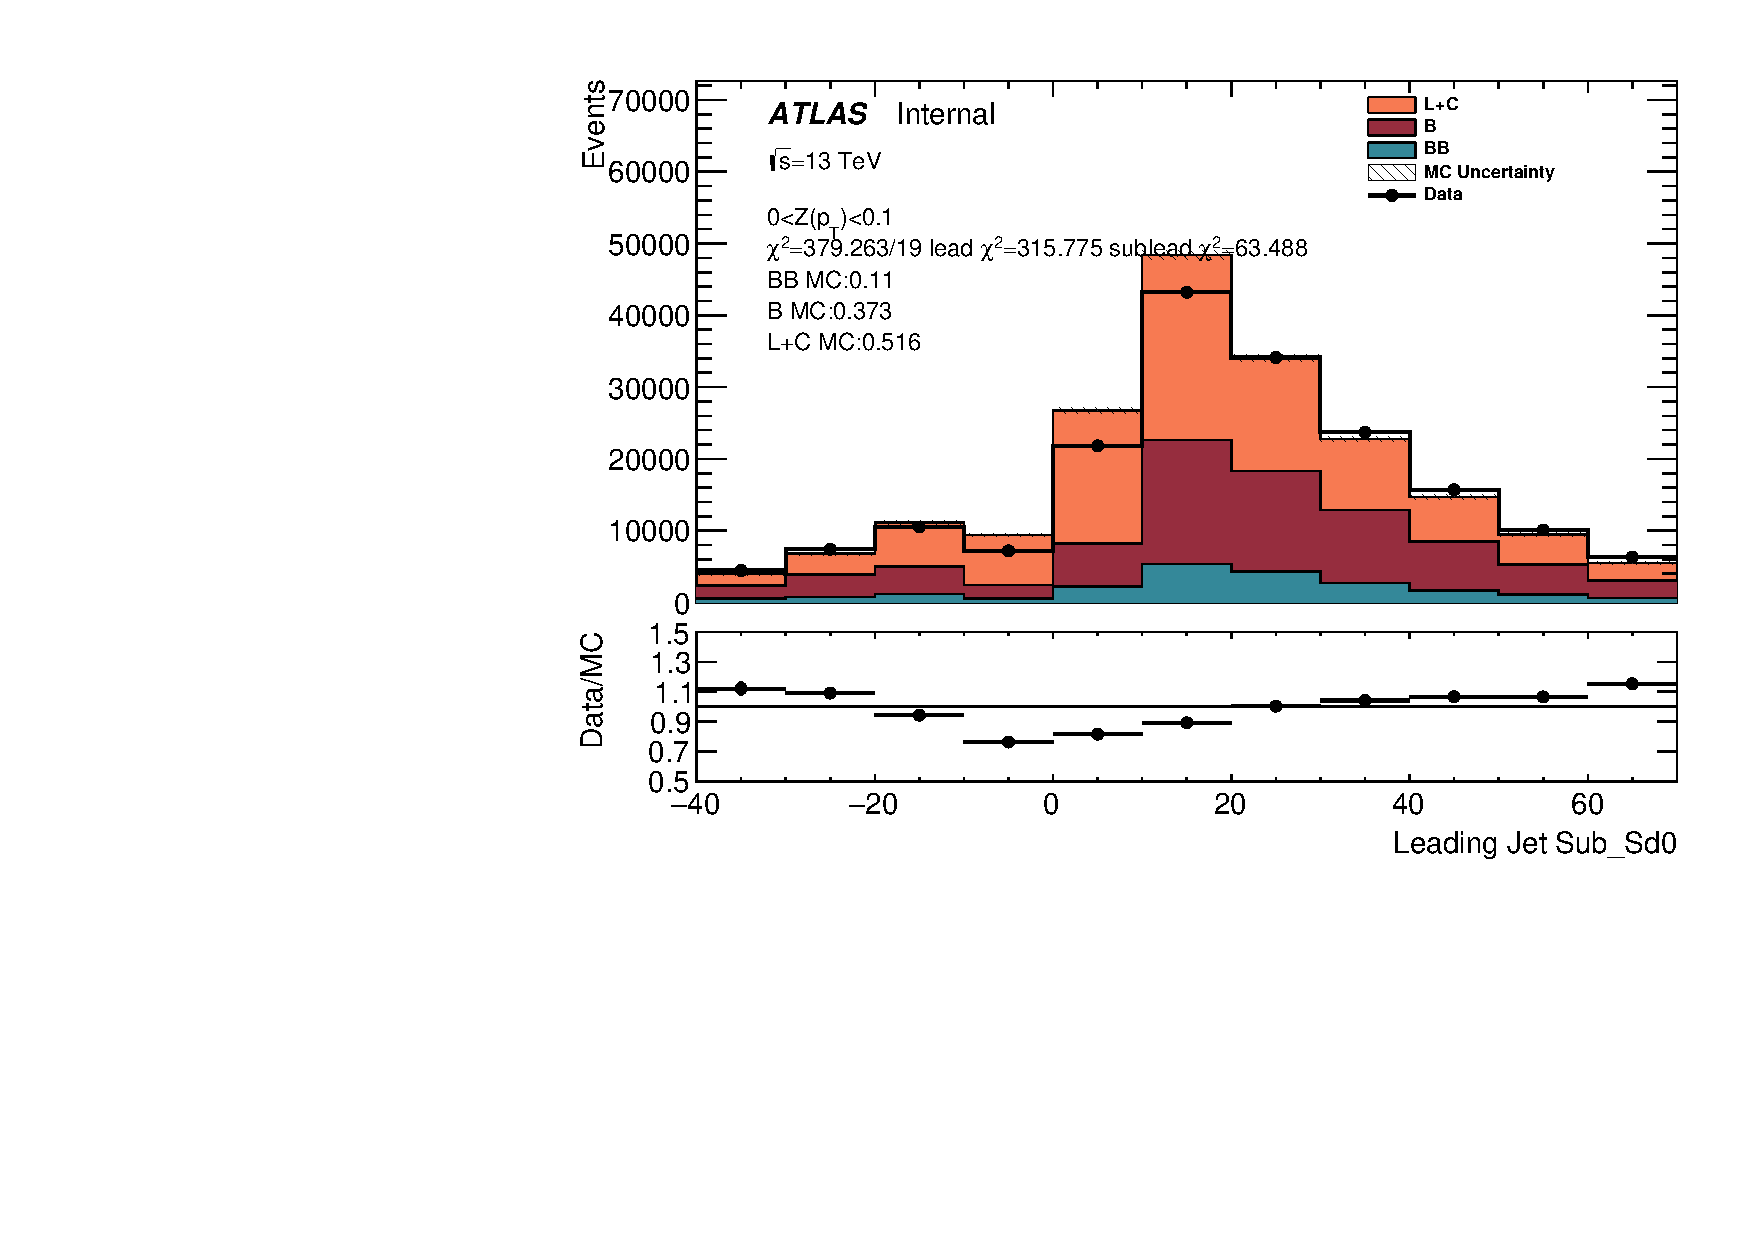
\includegraphics[width=0.32\textwidth]{figures/gbb/Sub_Sd0_Fits/Canv_PreFit_0-Zp_T-01_LpT_INF_SpT_INF_coarse_x.pdf}
 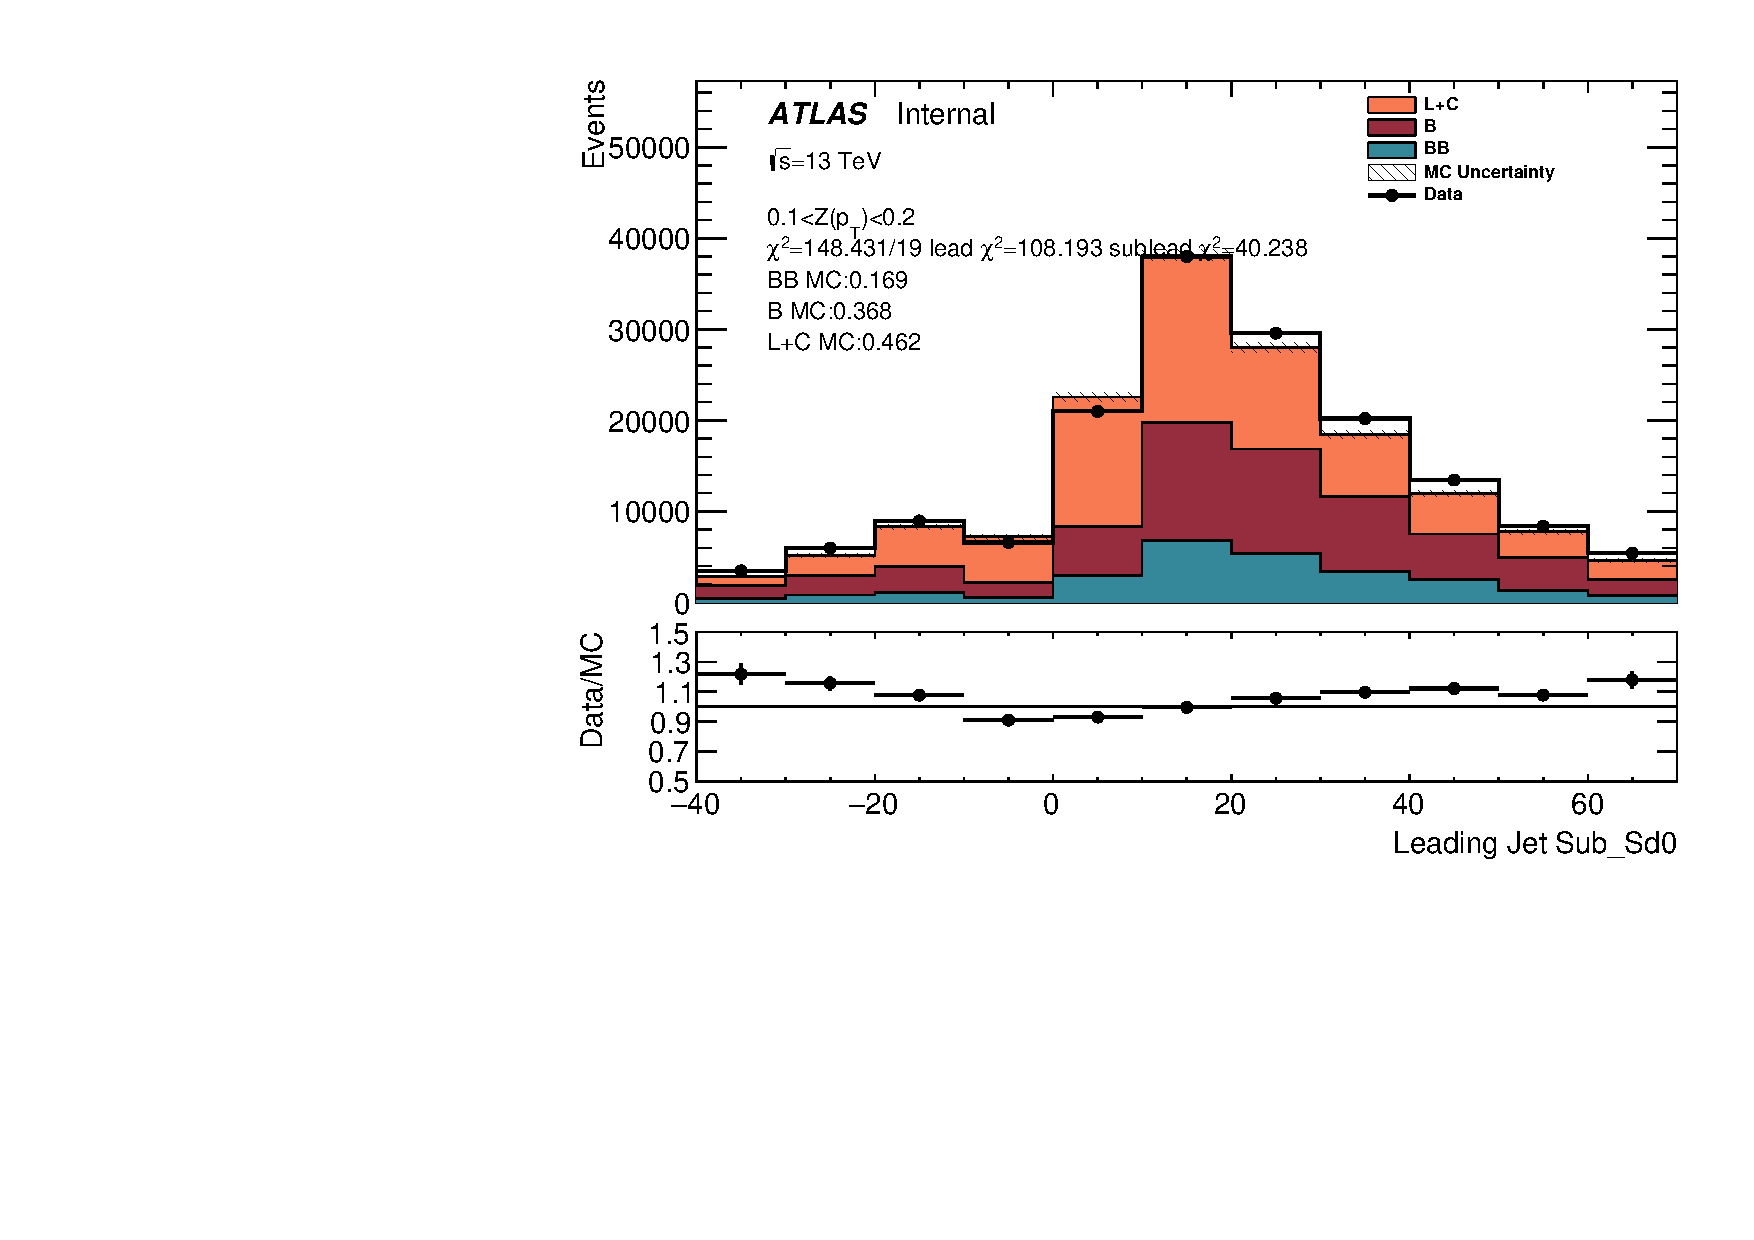
\includegraphics[width=0.32\textwidth]{figures/gbb/Sub_Sd0_Fits/Canv_PreFit_01-Zp_T-02_LpT_INF_SpT_INF_coarse_x.pdf}
 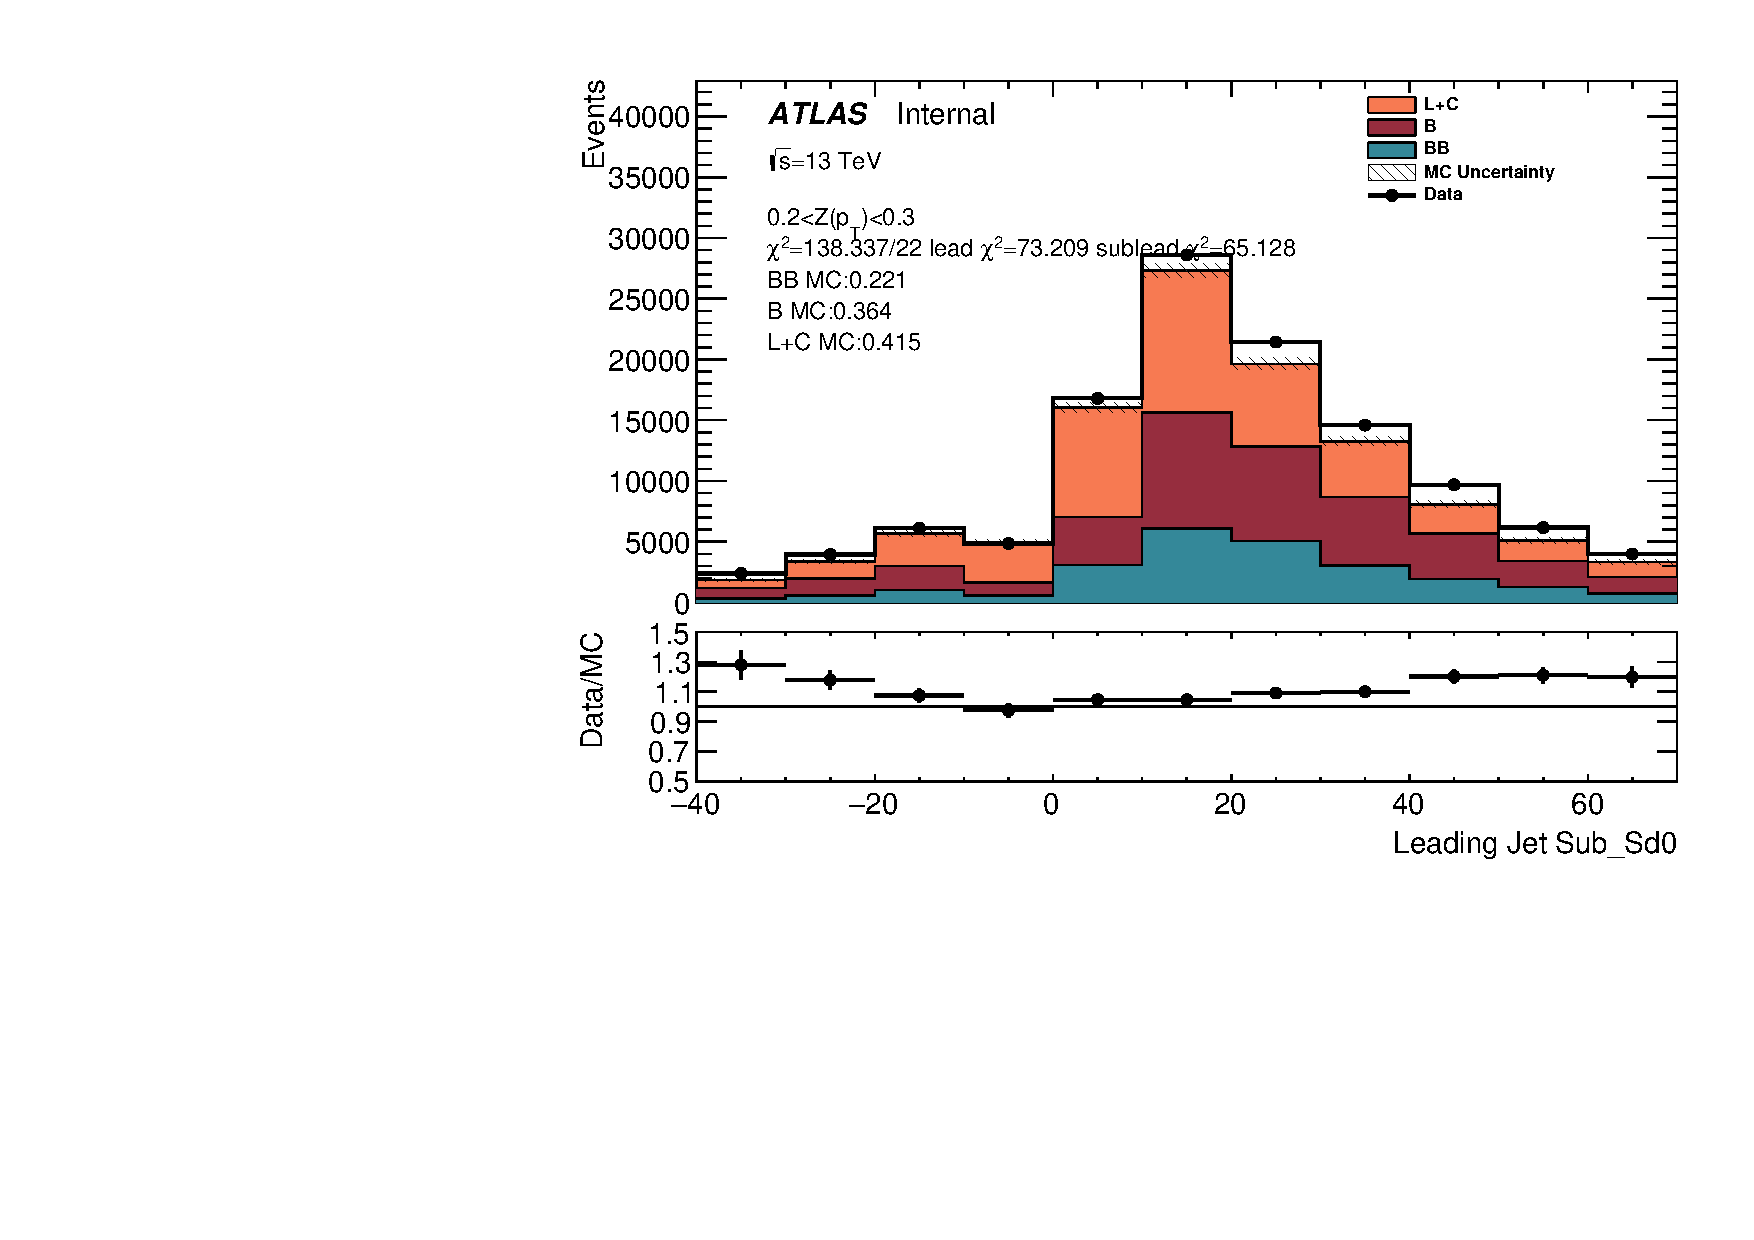
\includegraphics[width=0.32\textwidth]{figures/gbb/Sub_Sd0_Fits/Canv_PreFit_02-Zp_T-03_LpT_INF_SpT_INF_coarse_x.pdf}\\
 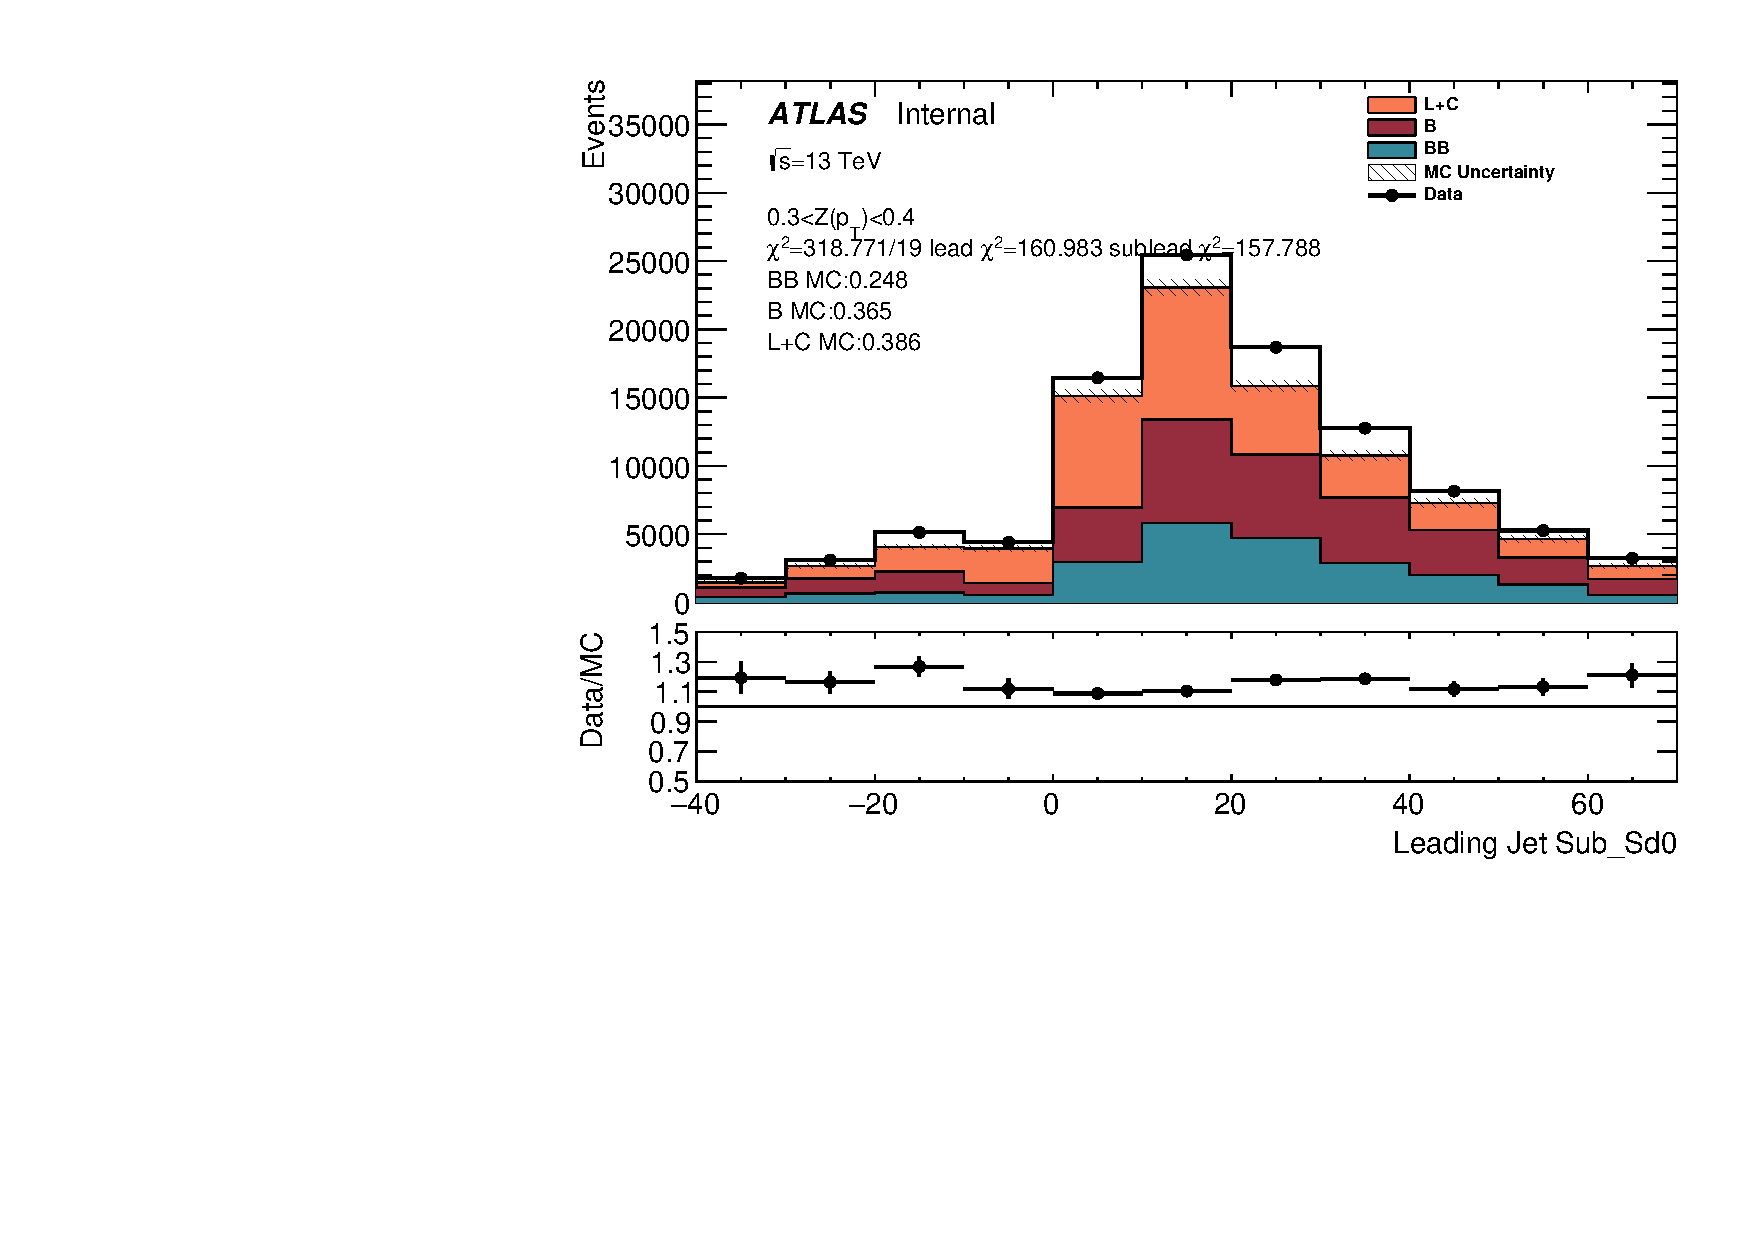
\includegraphics[width=0.32\textwidth]{figures/gbb/Sub_Sd0_Fits/Canv_PreFit_03-Zp_T-04_LpT_INF_SpT_INF_coarse_x.pdf}
 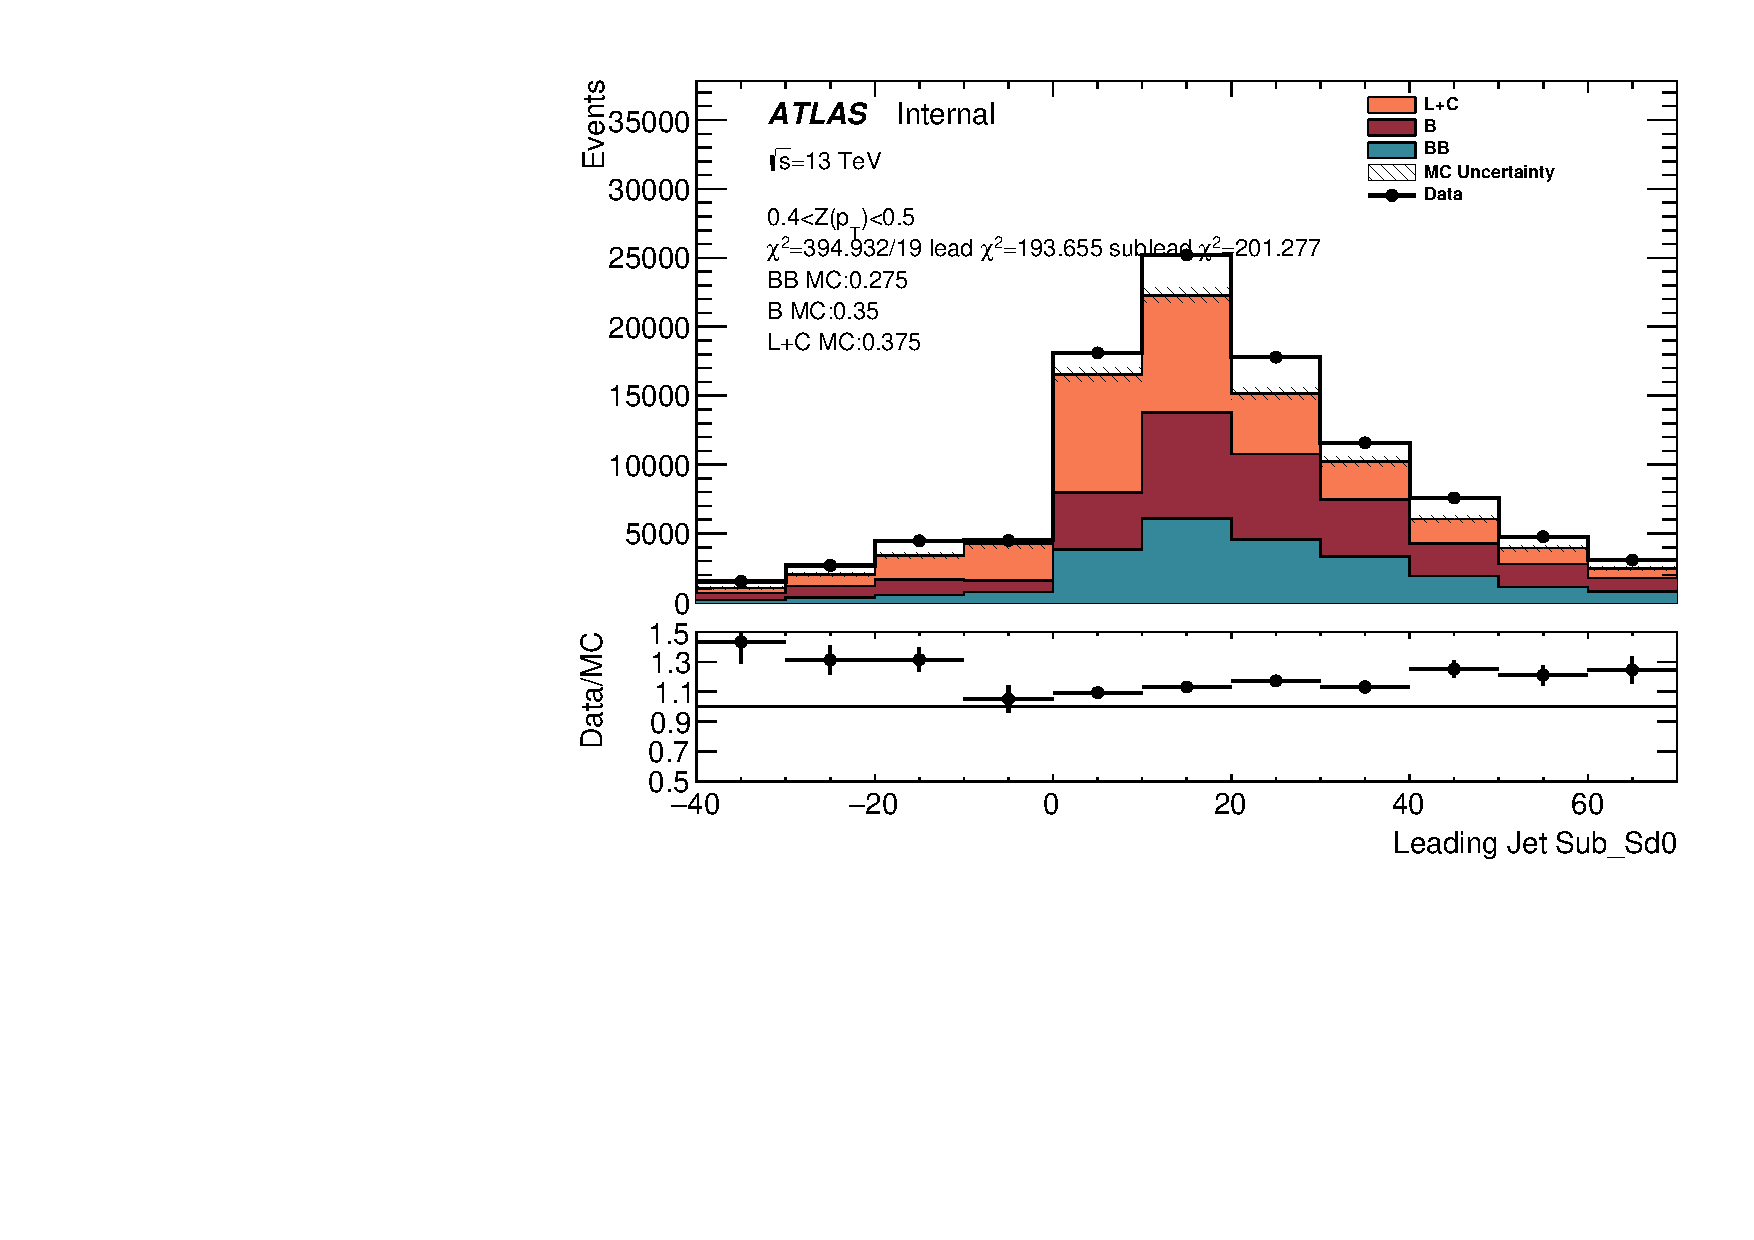
\includegraphics[width=0.32\textwidth]{figures/gbb/Sub_Sd0_Fits/Canv_PreFit_04-Zp_T-05_LpT_INF_SpT_INF_coarse_x.pdf}

\caption{Pre-fit \subsdzero distributions of the leading track jet in bins of \zpt. }
  \label{fig:ZpT-prefits-leading}
\end{figure}


\begin{figure}[htbp]
  \centering
 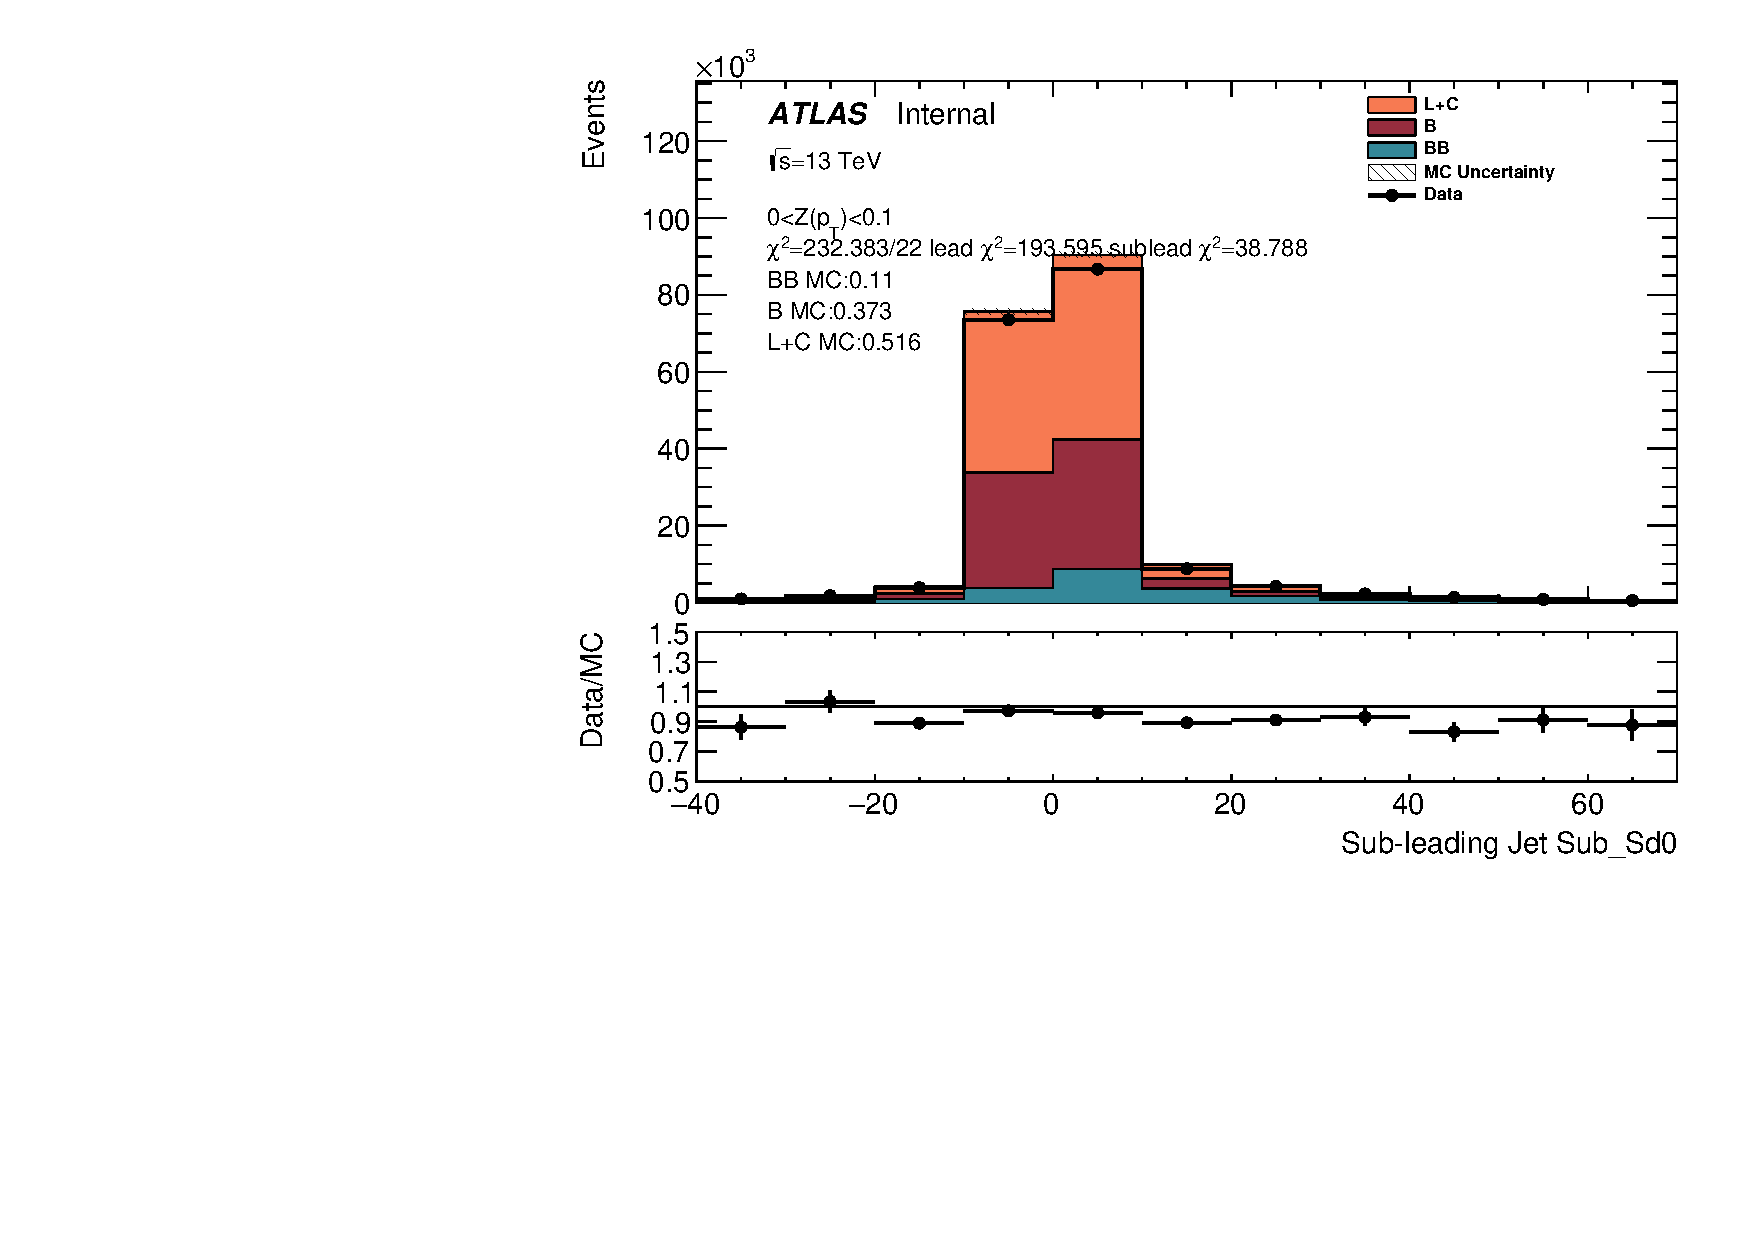
\includegraphics[width=0.32\textwidth]{figures/gbb/Sub_Sd0_Fits/Canv_PreFit_0-Zp_T-01_LpT_INF_SpT_INF_coarse_y.pdf}
 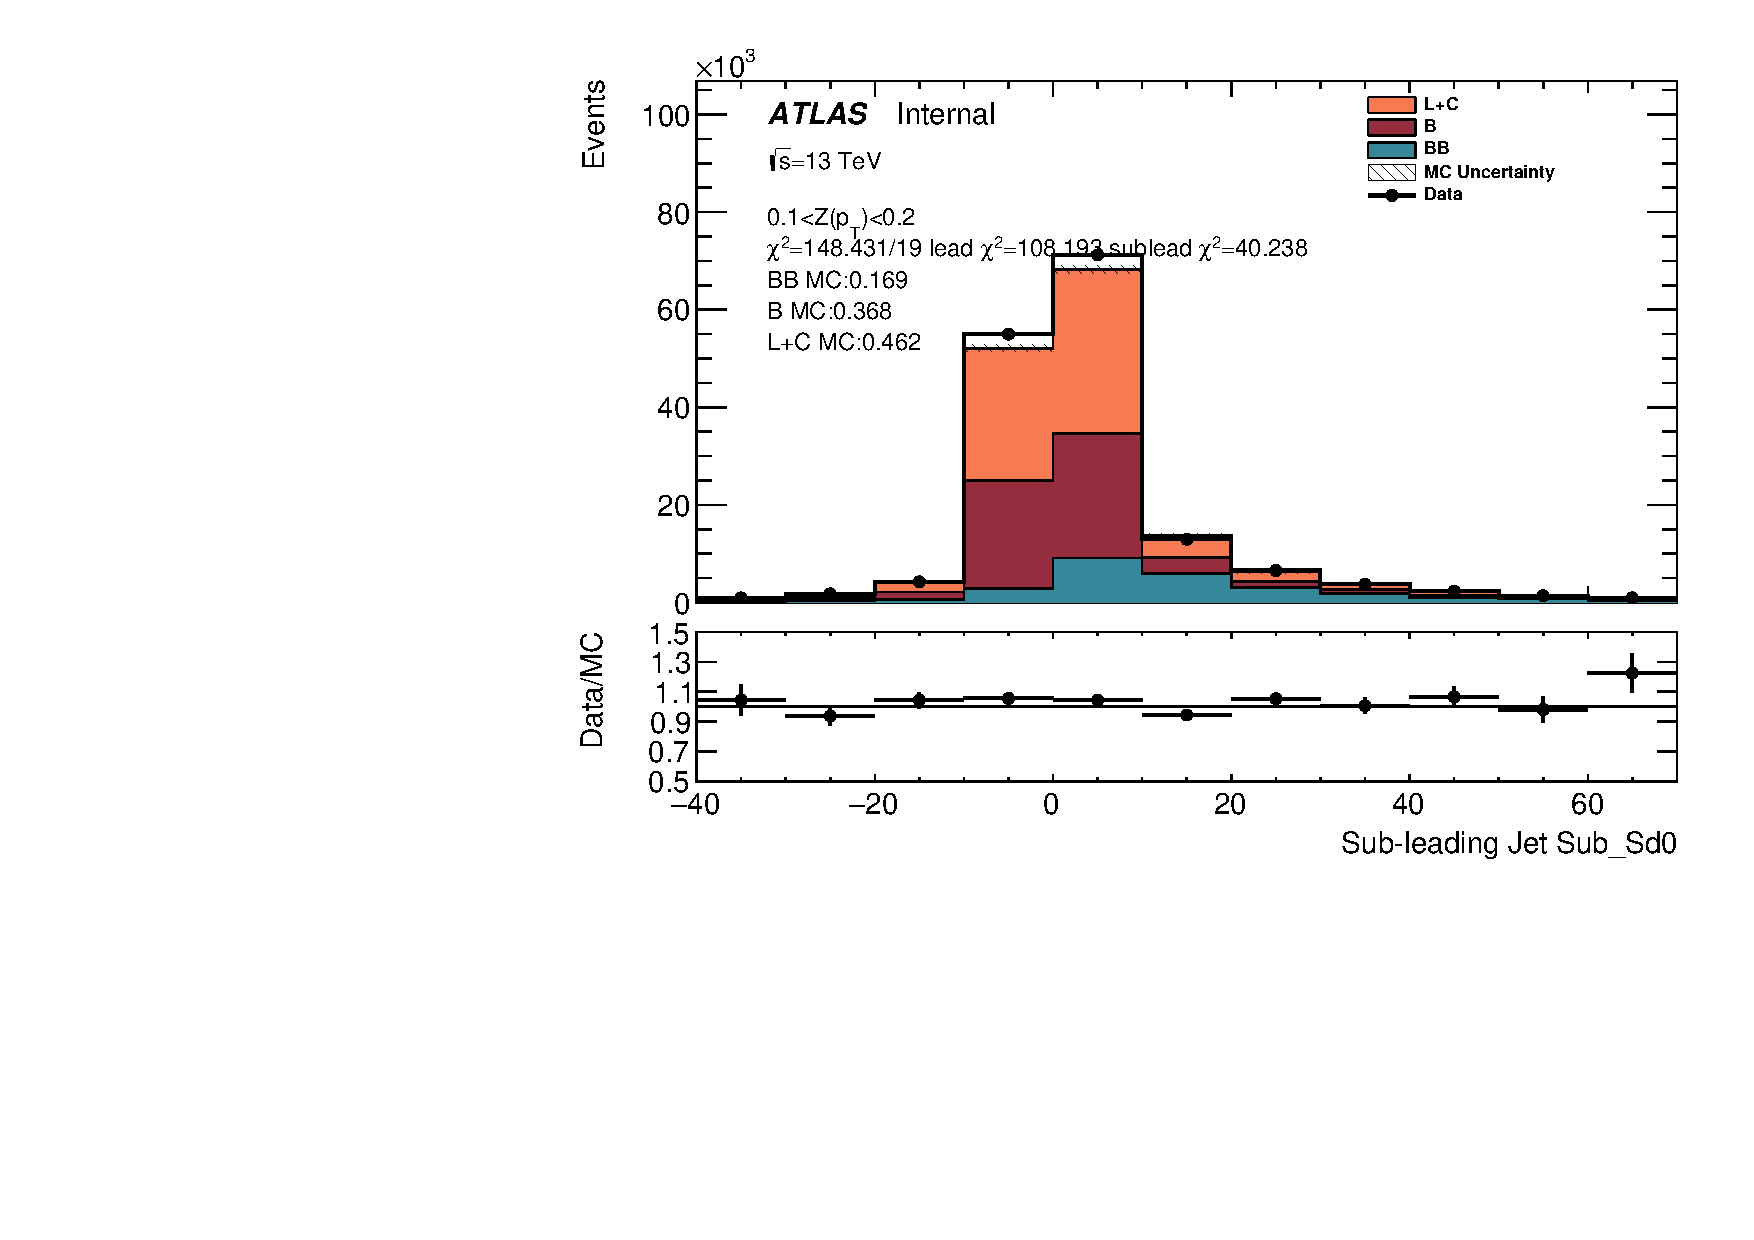
\includegraphics[width=0.32\textwidth]{figures/gbb/Sub_Sd0_Fits/Canv_PreFit_01-Zp_T-02_LpT_INF_SpT_INF_coarse_y.pdf}
 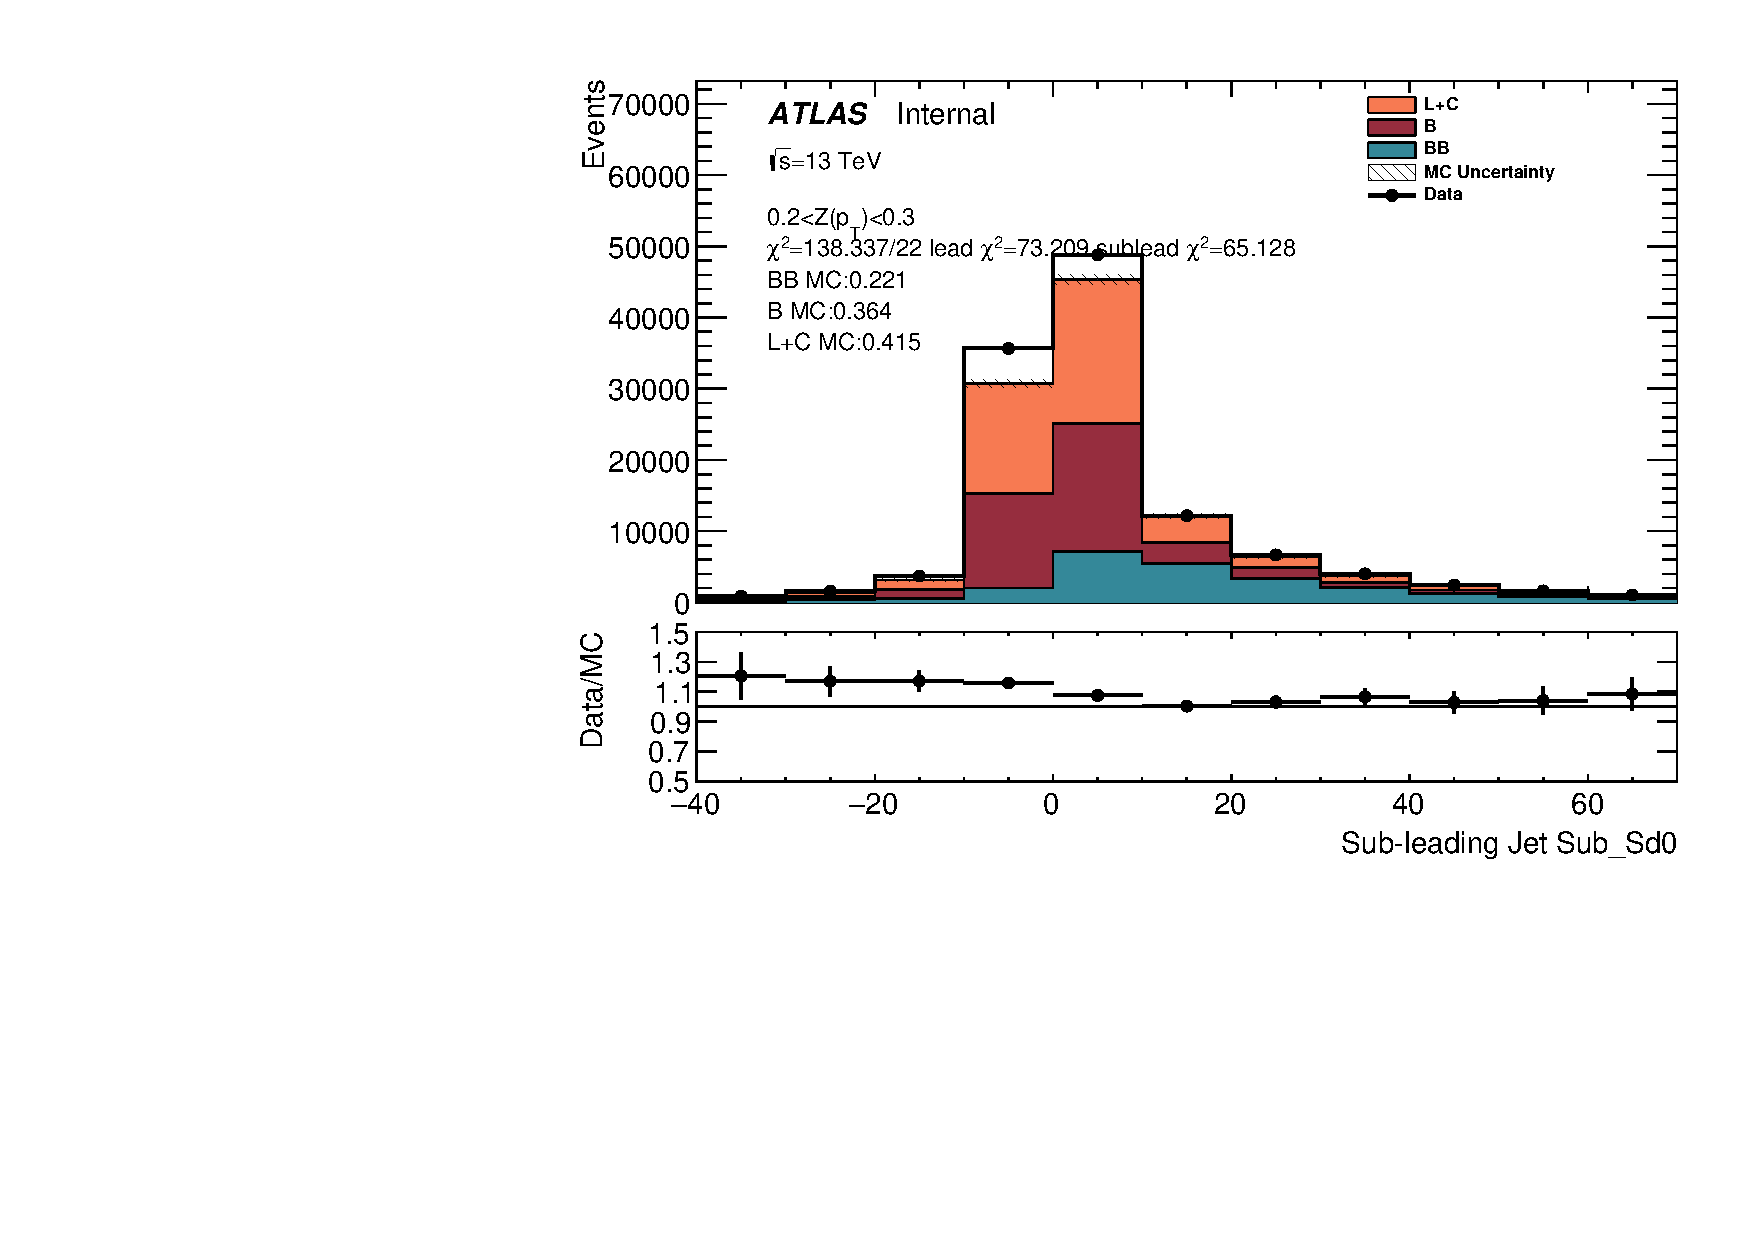
\includegraphics[width=0.32\textwidth]{figures/gbb/Sub_Sd0_Fits/Canv_PreFit_02-Zp_T-03_LpT_INF_SpT_INF_coarse_y.pdf}\\
 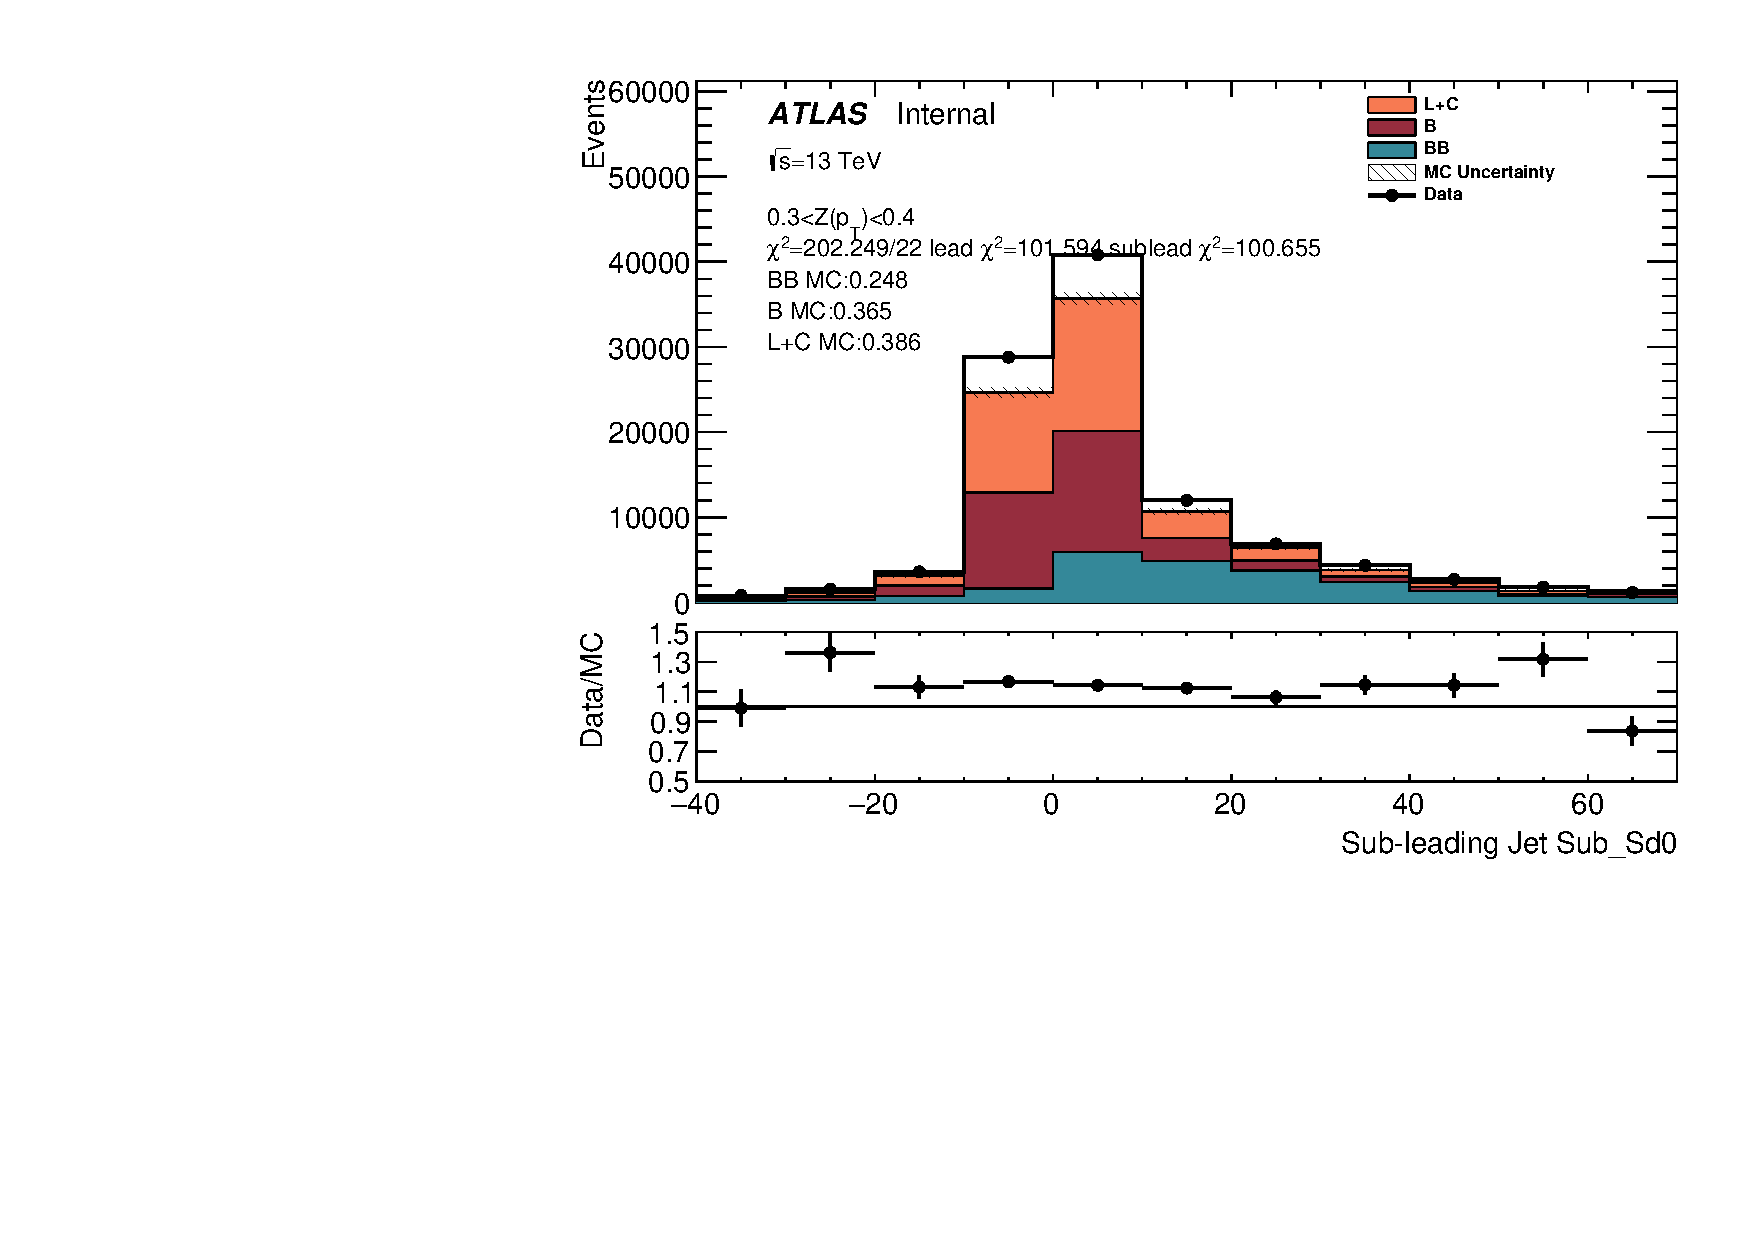
\includegraphics[width=0.32\textwidth]{figures/gbb/Sub_Sd0_Fits/Canv_PreFit_03-Zp_T-04_LpT_INF_SpT_INF_coarse_y.pdf}
 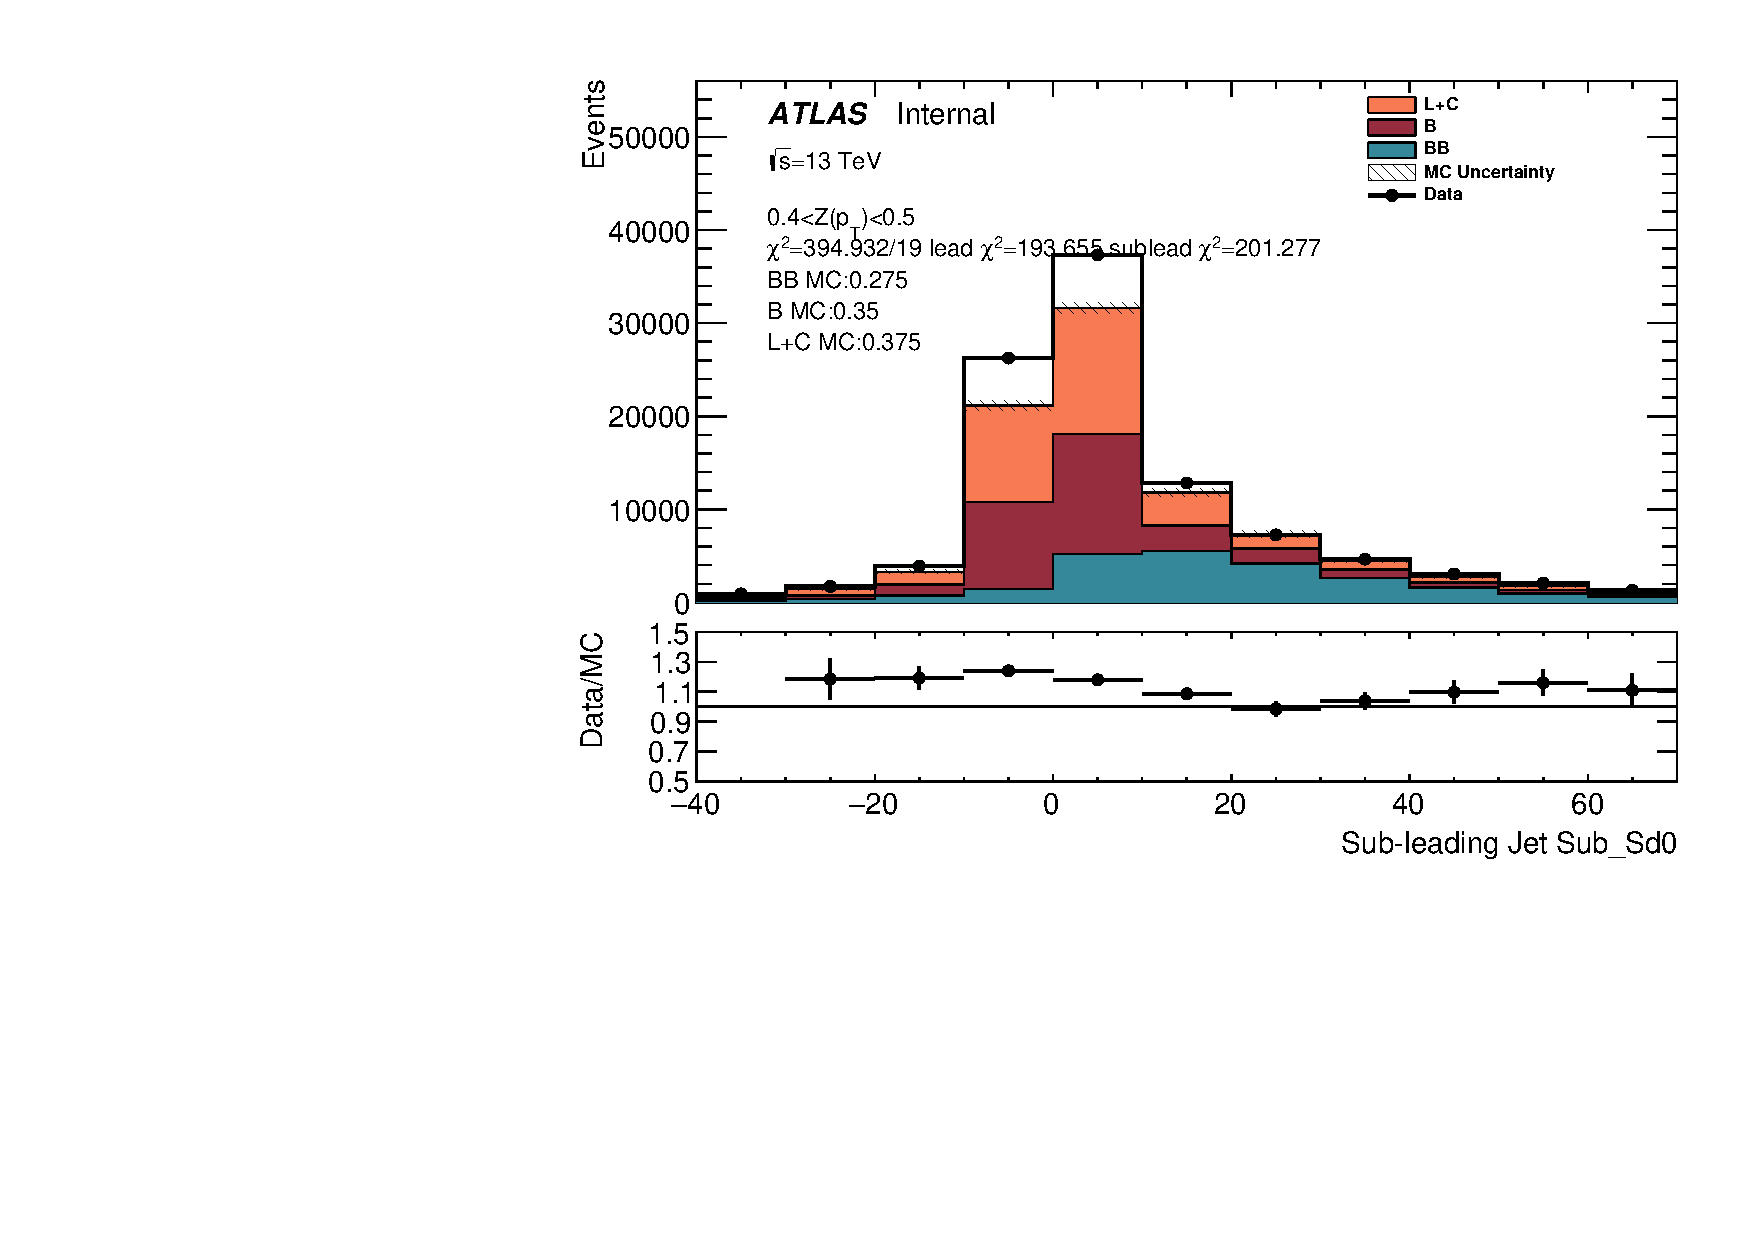
\includegraphics[width=0.32\textwidth]{figures/gbb/Sub_Sd0_Fits/Canv_PreFit_04-Zp_T-05_LpT_INF_SpT_INF_coarse_y.pdf}

\caption{Pre-fit \subsdzero distributions of the sub-leading track jet in bins of \zpt. }
  \label{fig:ZpT-prefits-subleading}
\end{figure}

\begin{figure}[htbp]
  \centering
 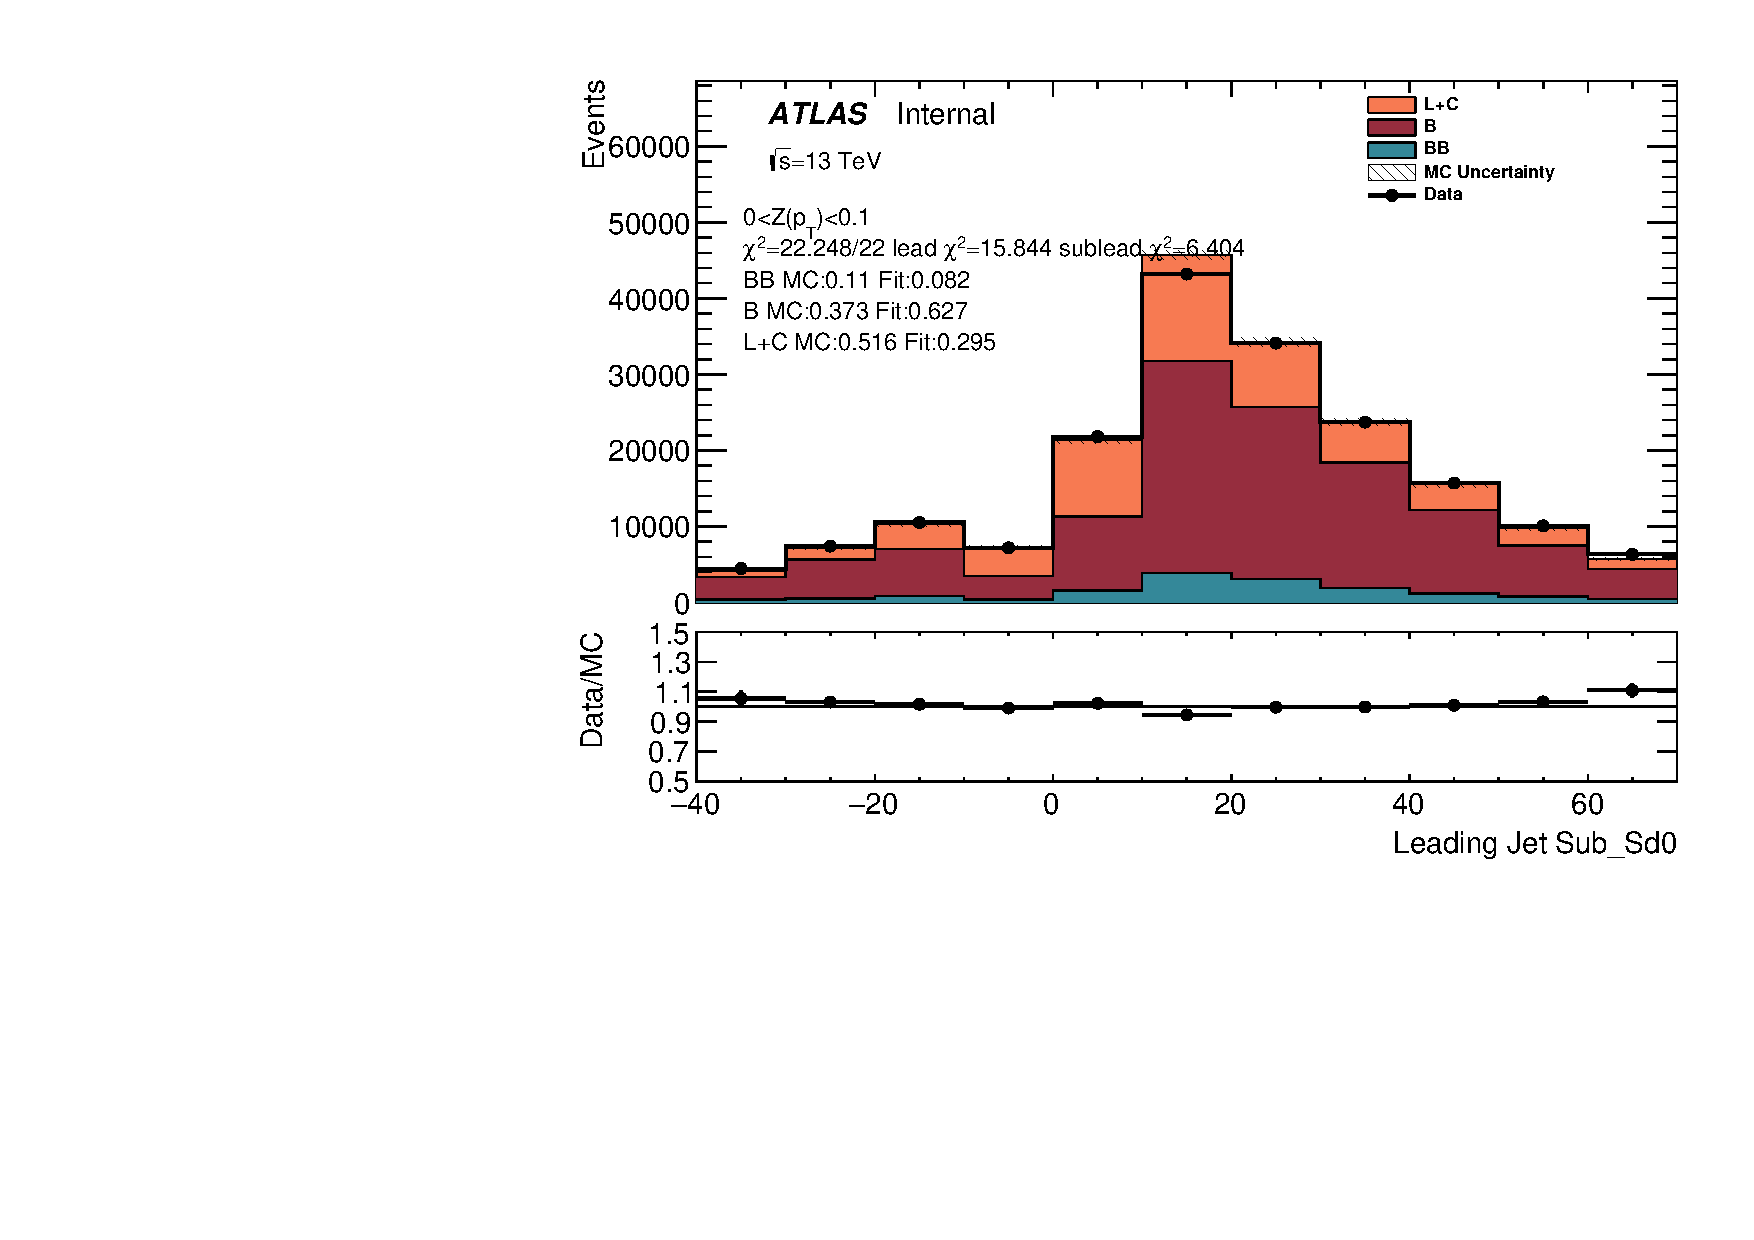
\includegraphics[width=0.32\textwidth]{figures/gbb/Sub_Sd0_Fits/Canv_Fit_0-Zp_T-01_LpT_INF_SpT_INF_coarse_x.pdf}
 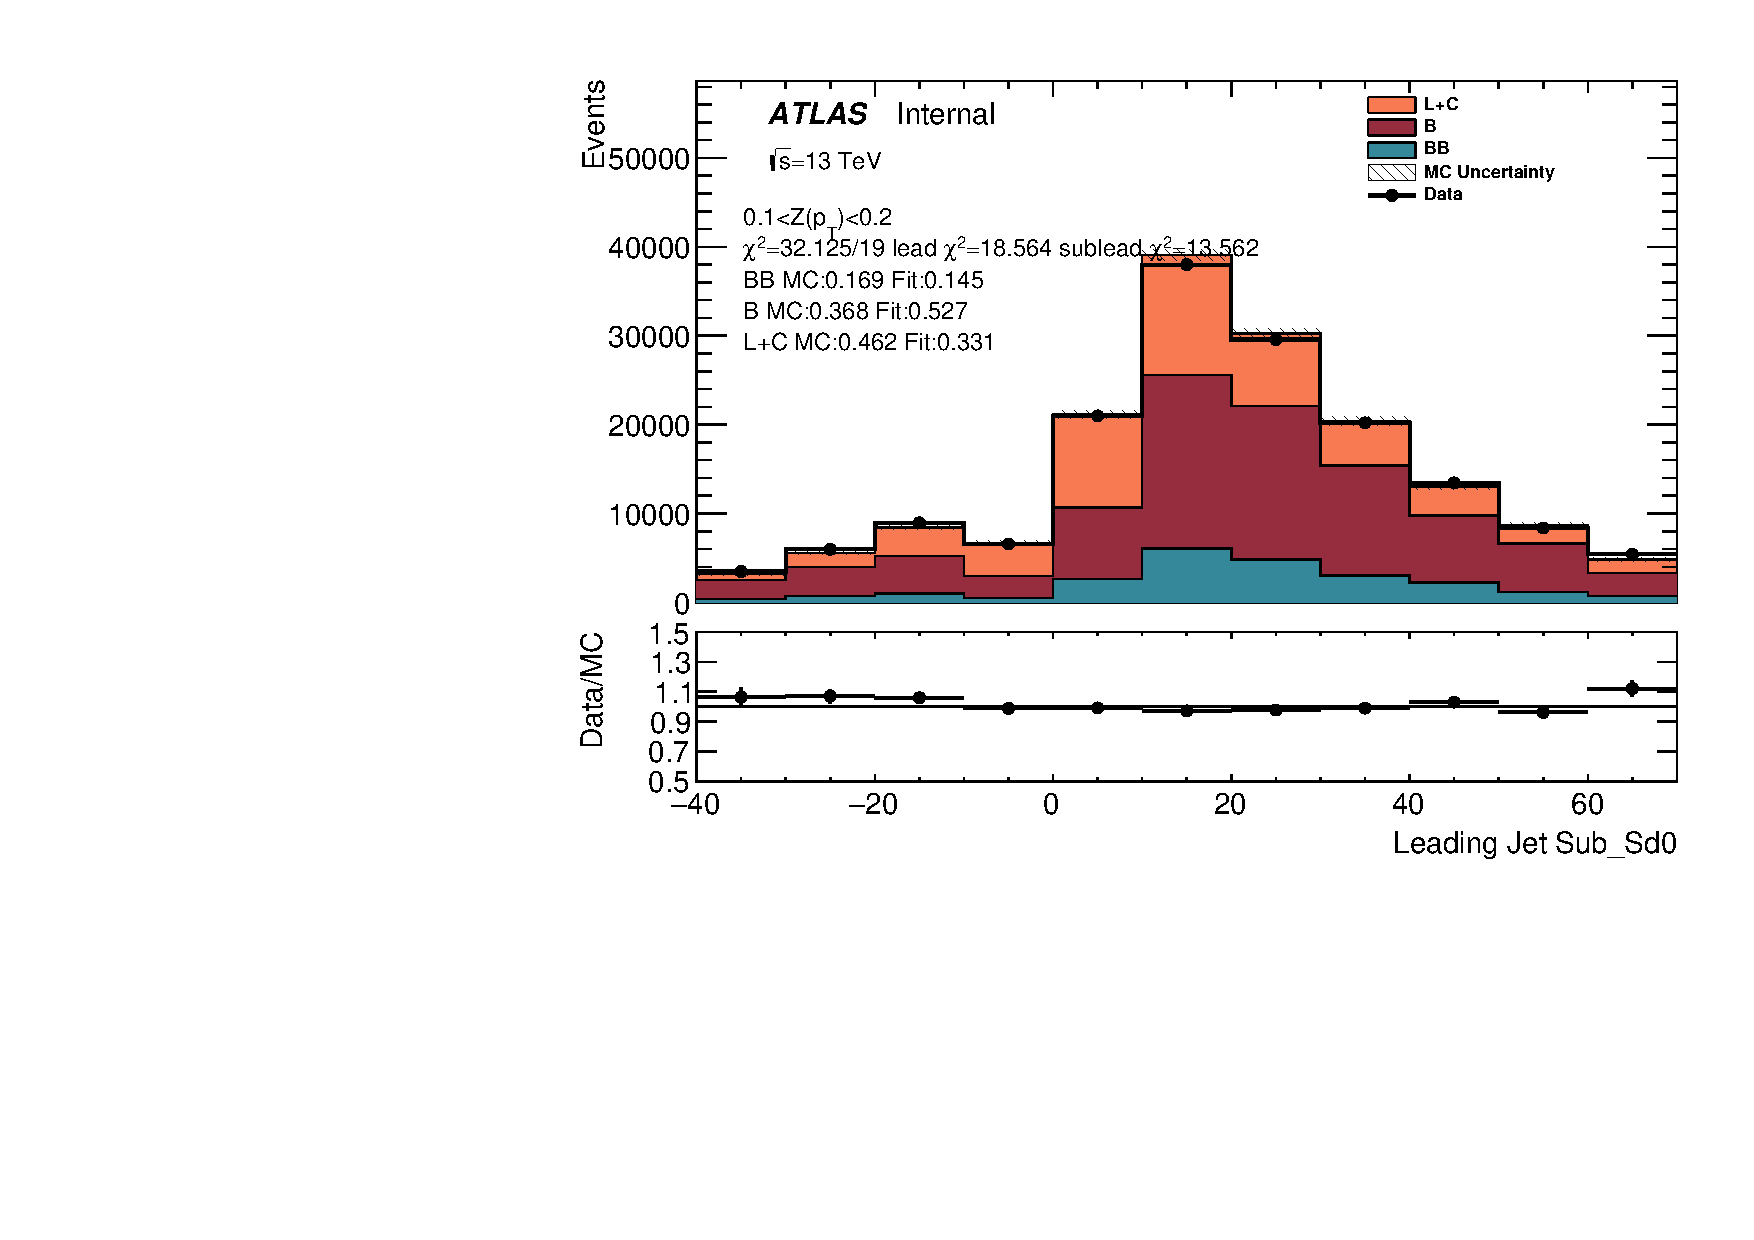
\includegraphics[width=0.32\textwidth]{figures/gbb/Sub_Sd0_Fits/Canv_Fit_01-Zp_T-02_LpT_INF_SpT_INF_coarse_x.pdf}
 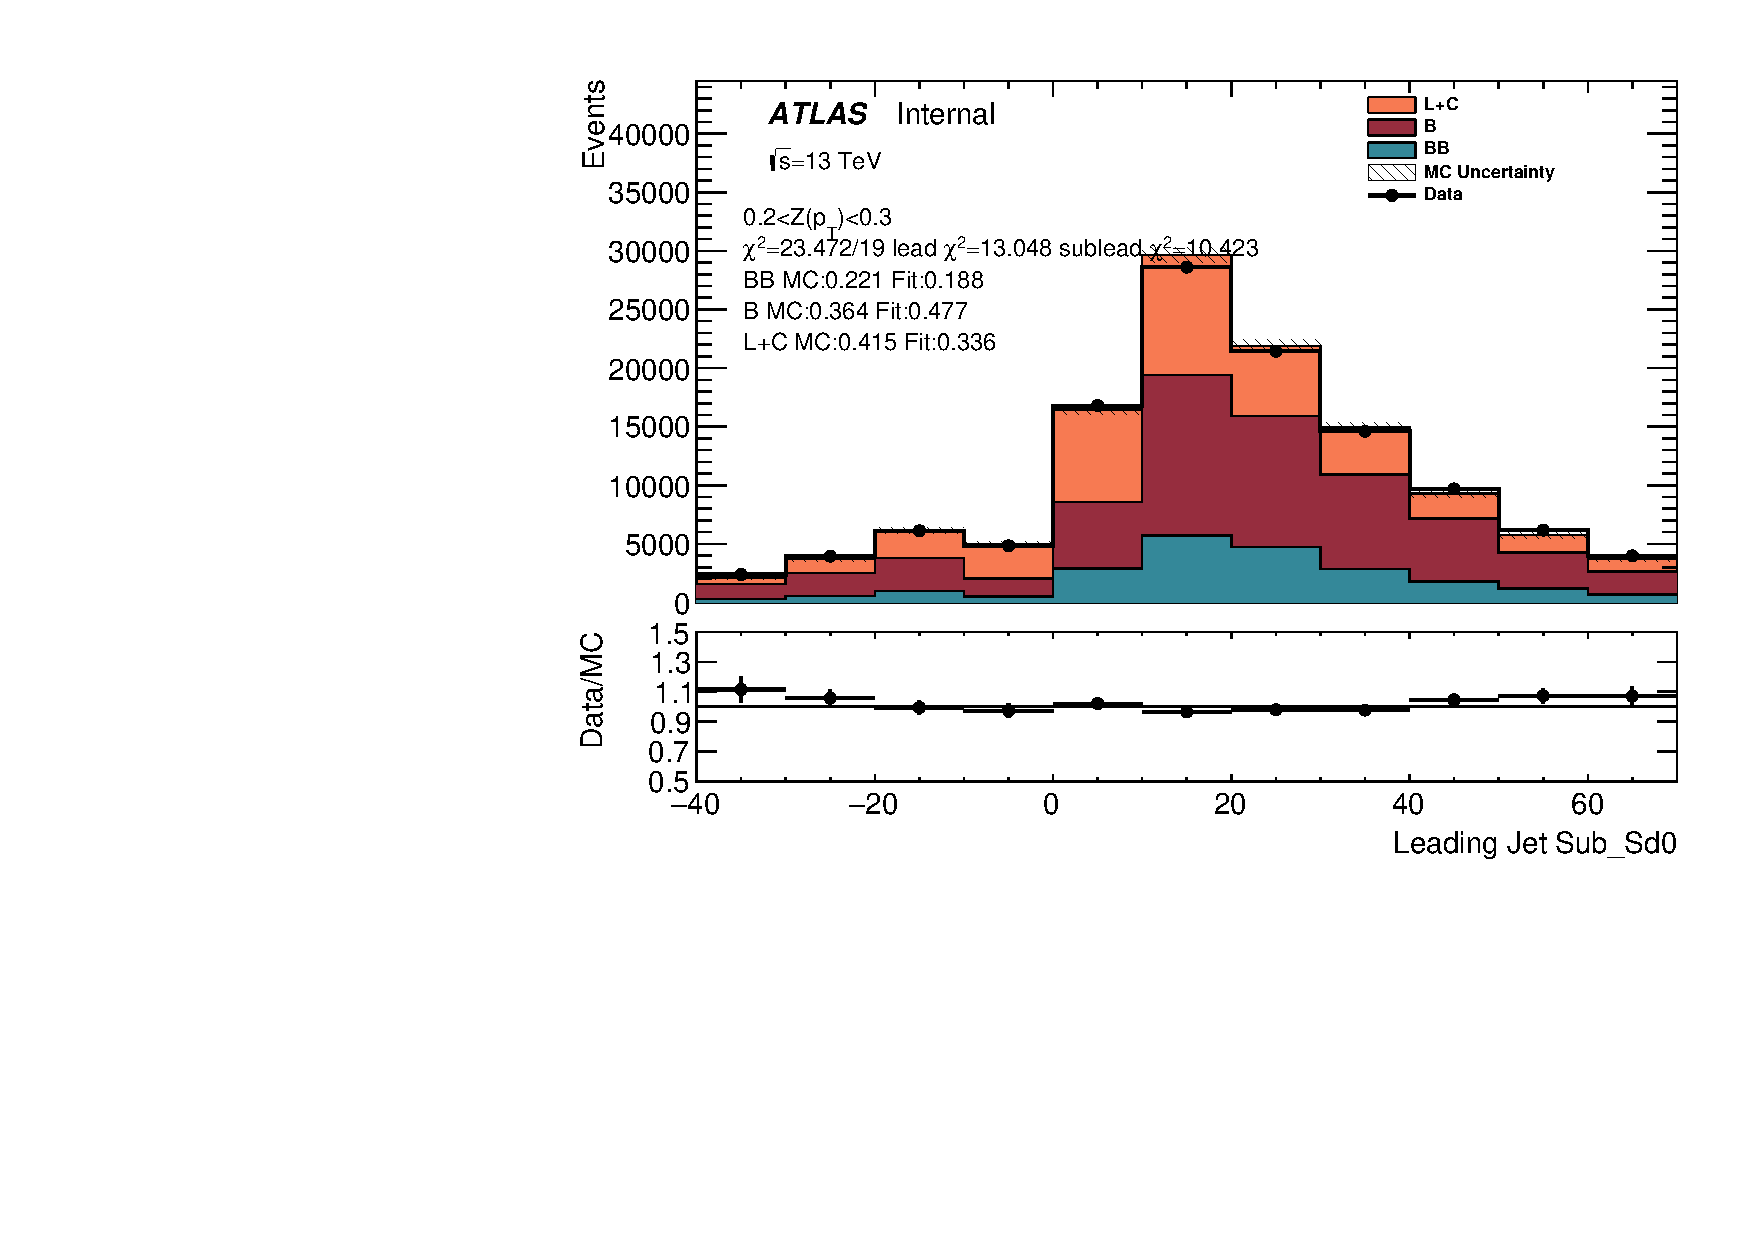
\includegraphics[width=0.32\textwidth]{figures/gbb/Sub_Sd0_Fits/Canv_Fit_02-Zp_T-03_LpT_INF_SpT_INF_coarse_x.pdf}\\
 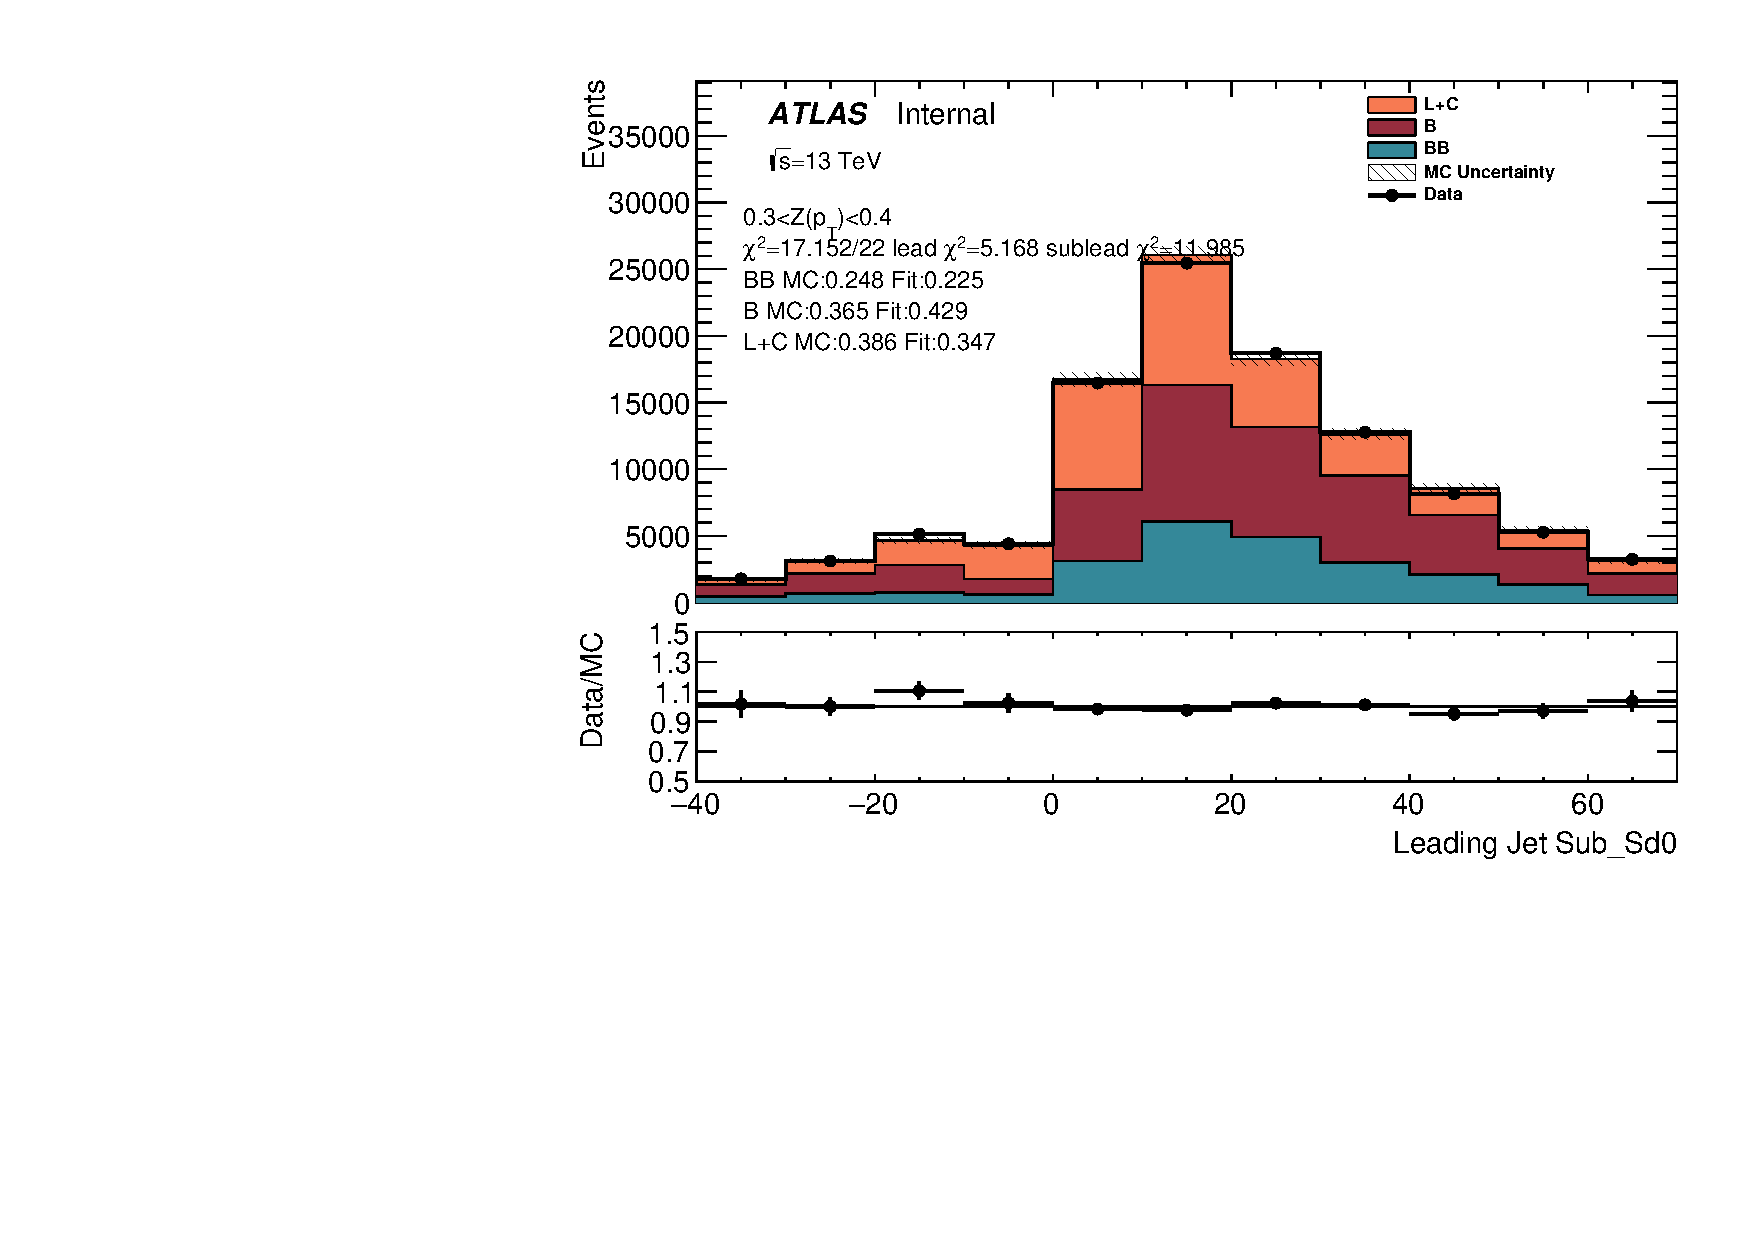
\includegraphics[width=0.32\textwidth]{figures/gbb/Sub_Sd0_Fits/Canv_Fit_03-Zp_T-04_LpT_INF_SpT_INF_coarse_x.pdf}
 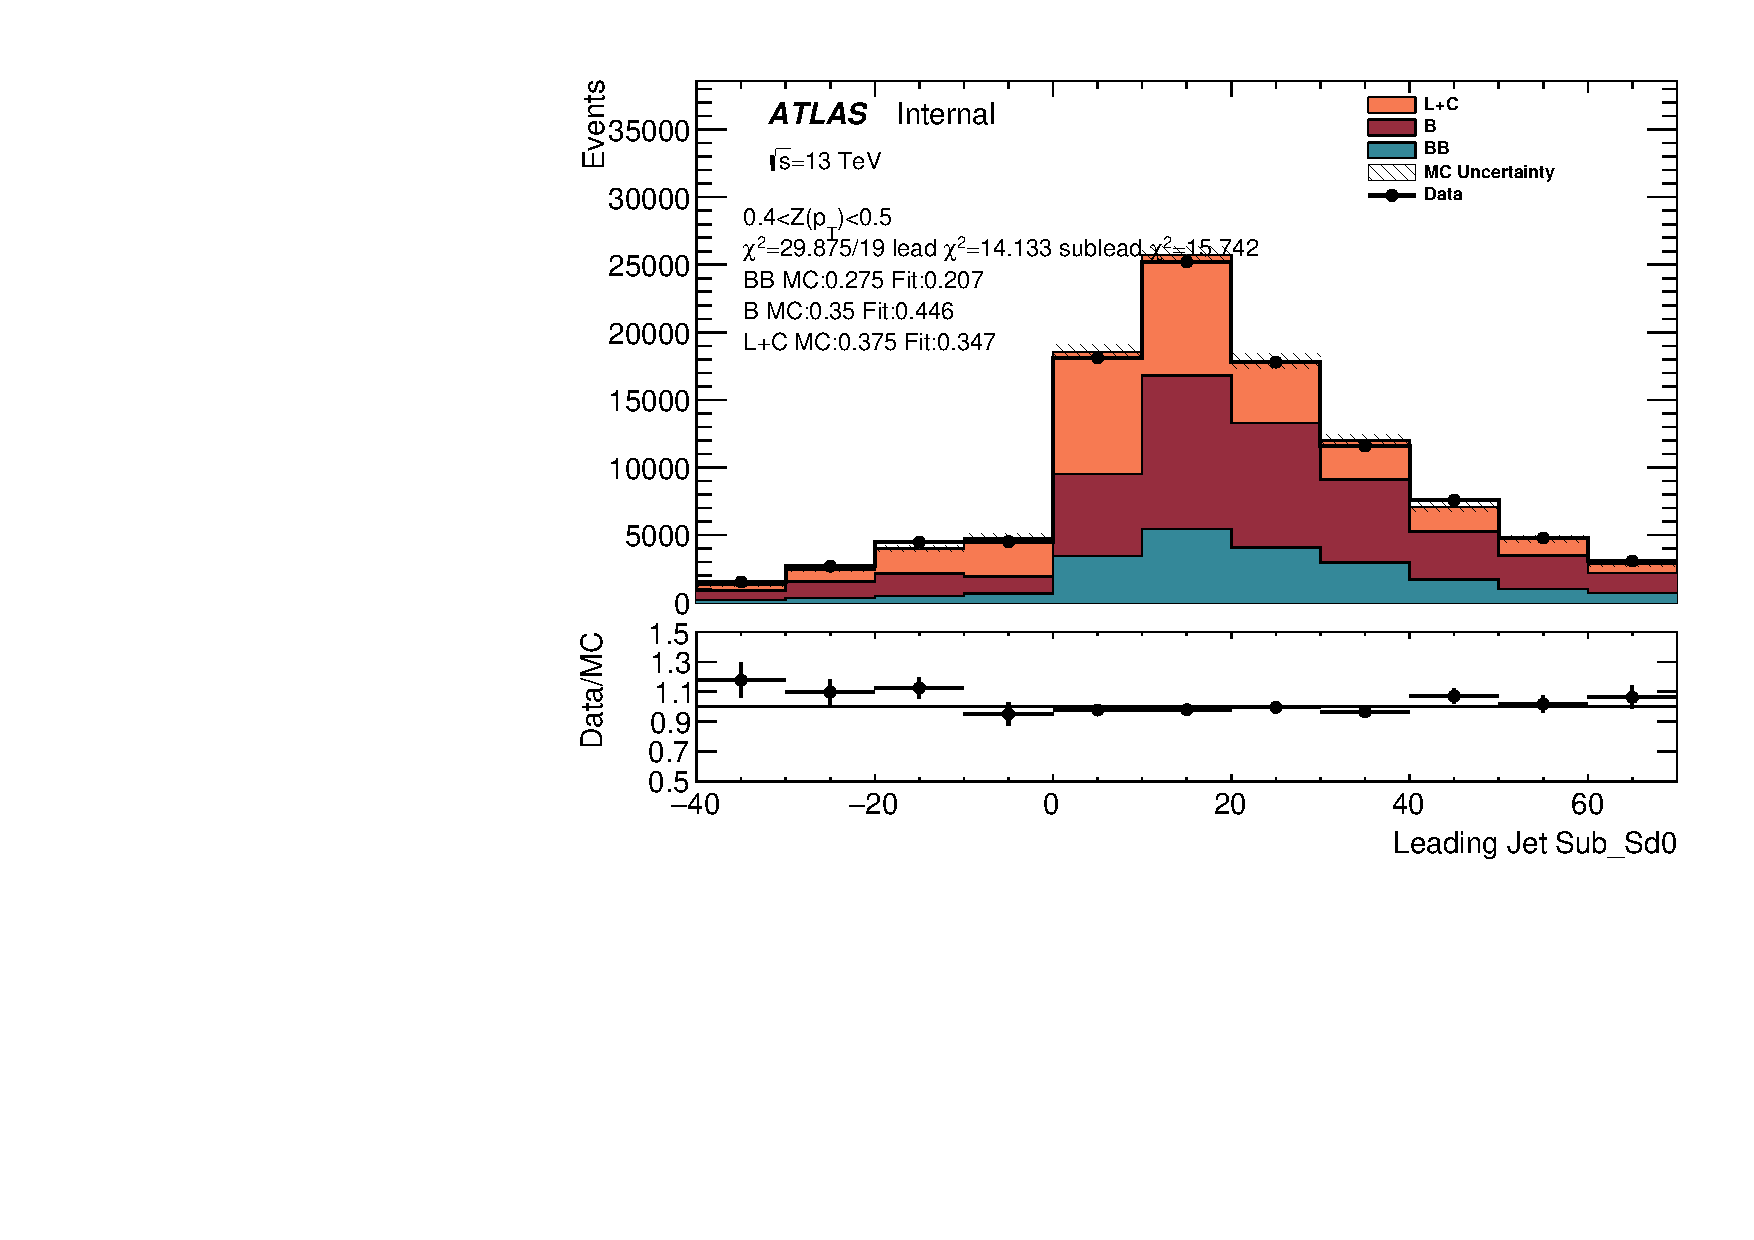
\includegraphics[width=0.32\textwidth]{figures/gbb/Sub_Sd0_Fits/Canv_Fit_04-Zp_T-05_LpT_INF_SpT_INF_coarse_x.pdf}


\caption{Post-fit \subsdzero distributions of the leading track jet in bins of \zpt. }
  \label{fig:ZpT-postfits-leading}
\end{figure}


\begin{figure}[htbp]
  \centering
 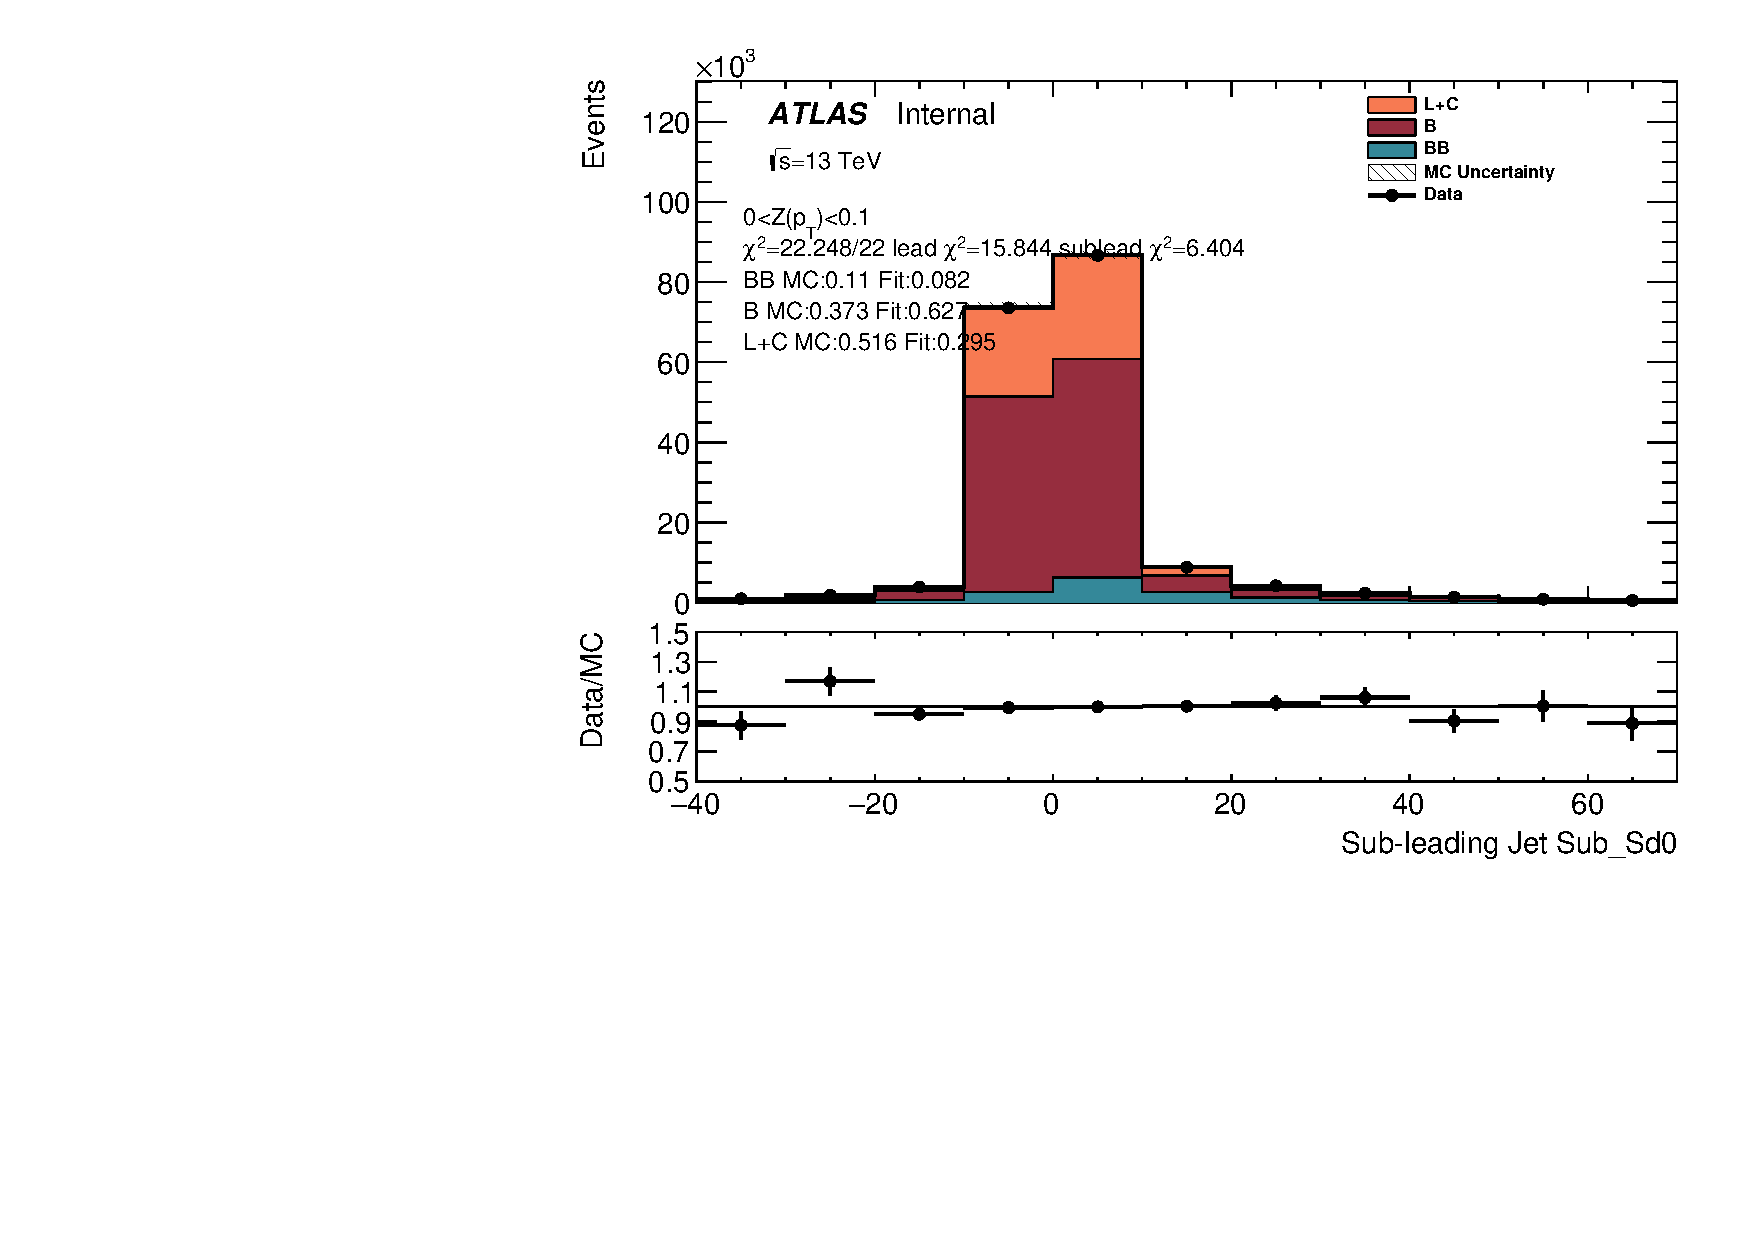
\includegraphics[width=0.32\textwidth]{figures/gbb/Sub_Sd0_Fits/Canv_Fit_0-Zp_T-01_LpT_INF_SpT_INF_coarse_y.pdf}
 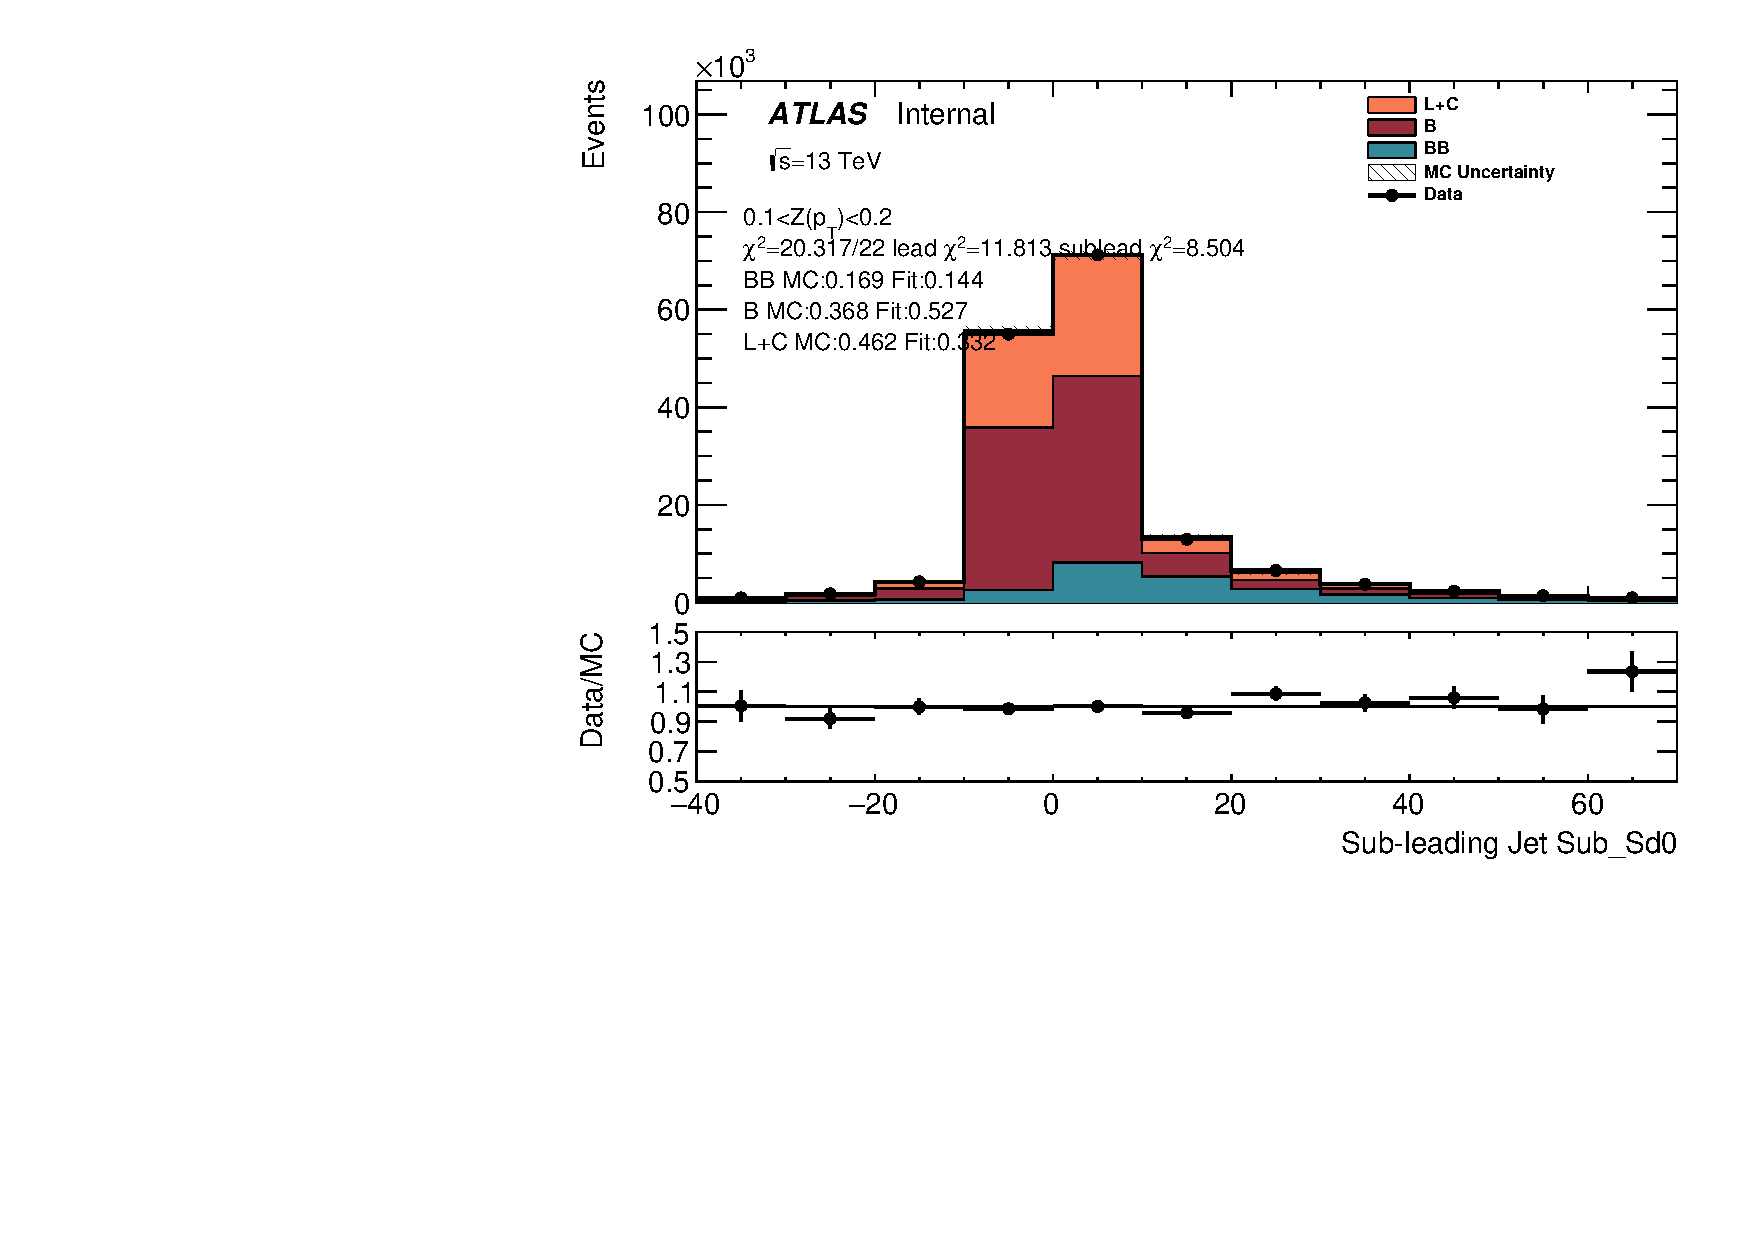
\includegraphics[width=0.32\textwidth]{figures/gbb/Sub_Sd0_Fits/Canv_Fit_01-Zp_T-02_LpT_INF_SpT_INF_coarse_y.pdf}
 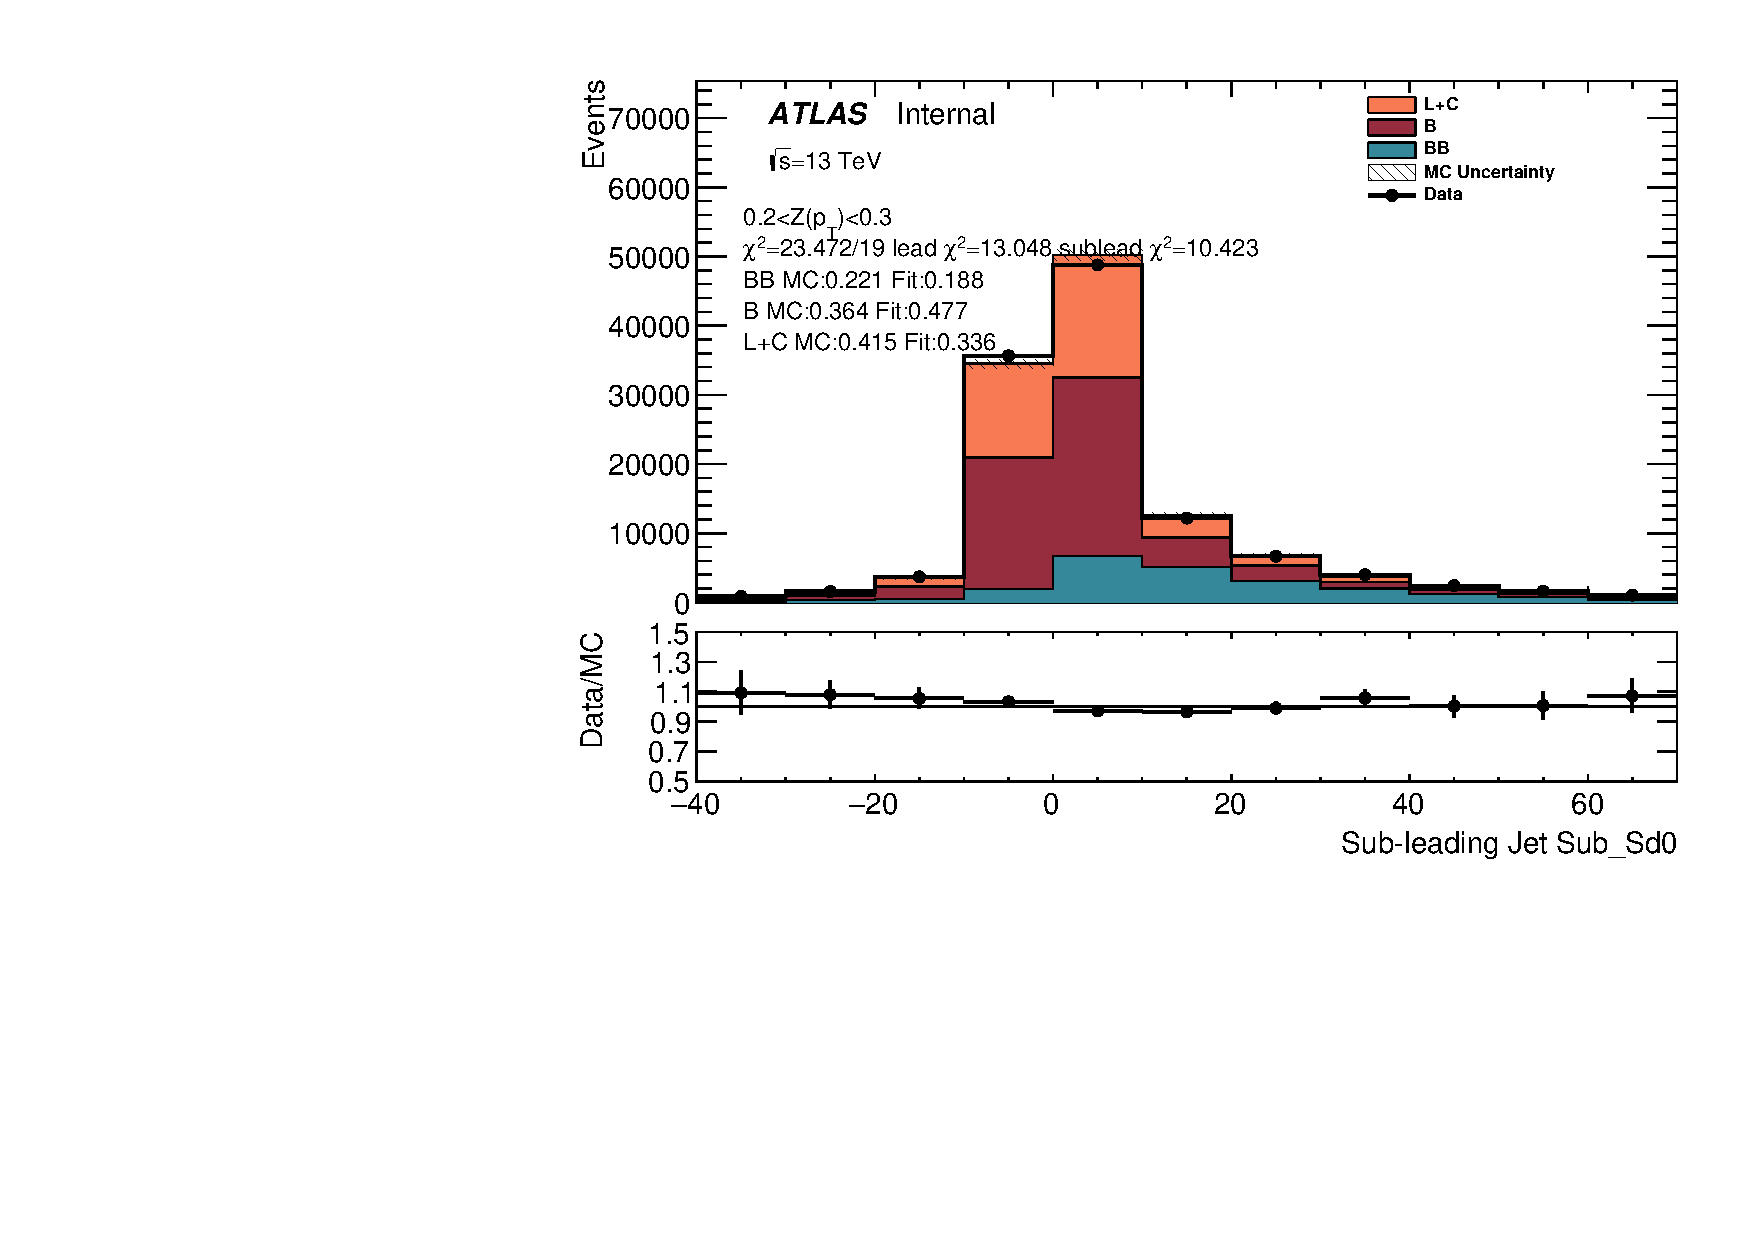
\includegraphics[width=0.32\textwidth]{figures/gbb/Sub_Sd0_Fits/Canv_Fit_02-Zp_T-03_LpT_INF_SpT_INF_coarse_y.pdf}\\
 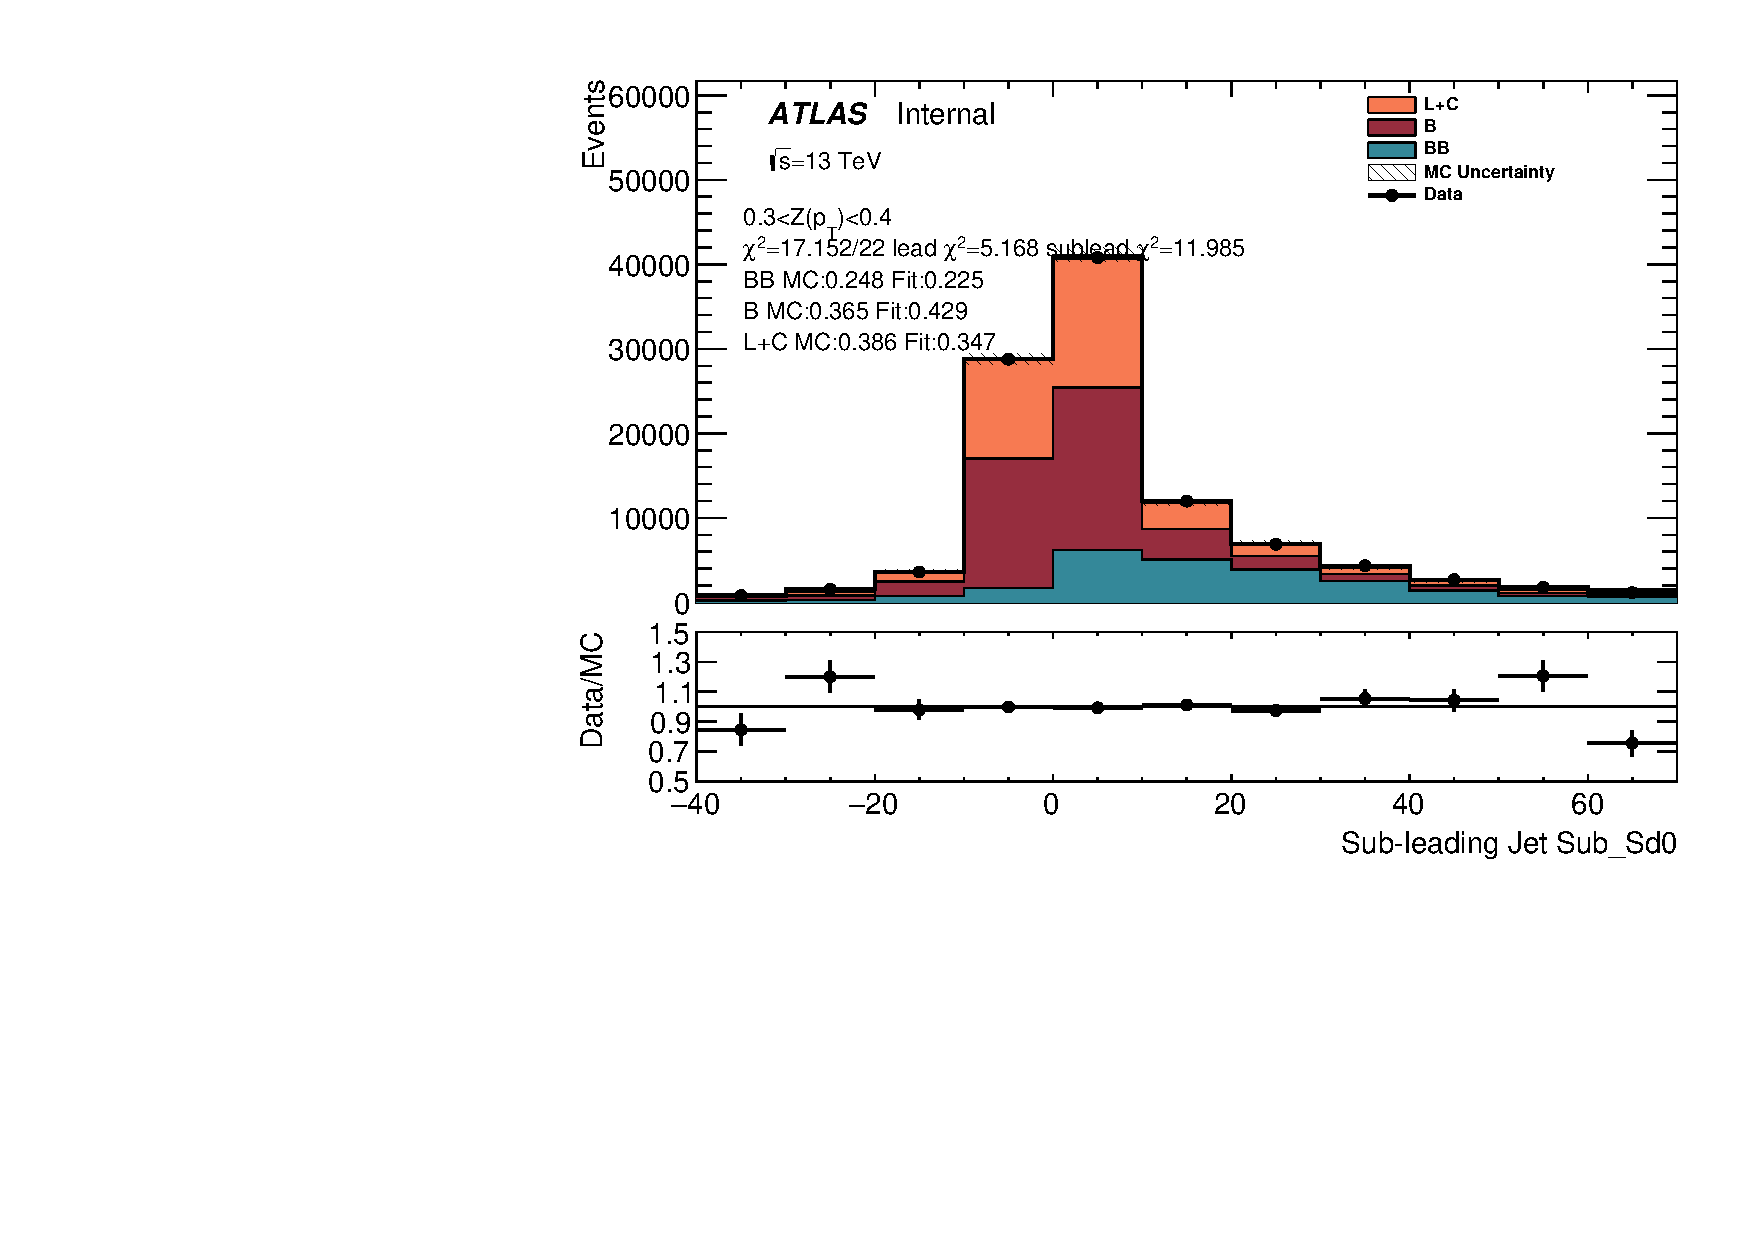
\includegraphics[width=0.32\textwidth]{figures/gbb/Sub_Sd0_Fits/Canv_Fit_03-Zp_T-04_LpT_INF_SpT_INF_coarse_y.pdf}
 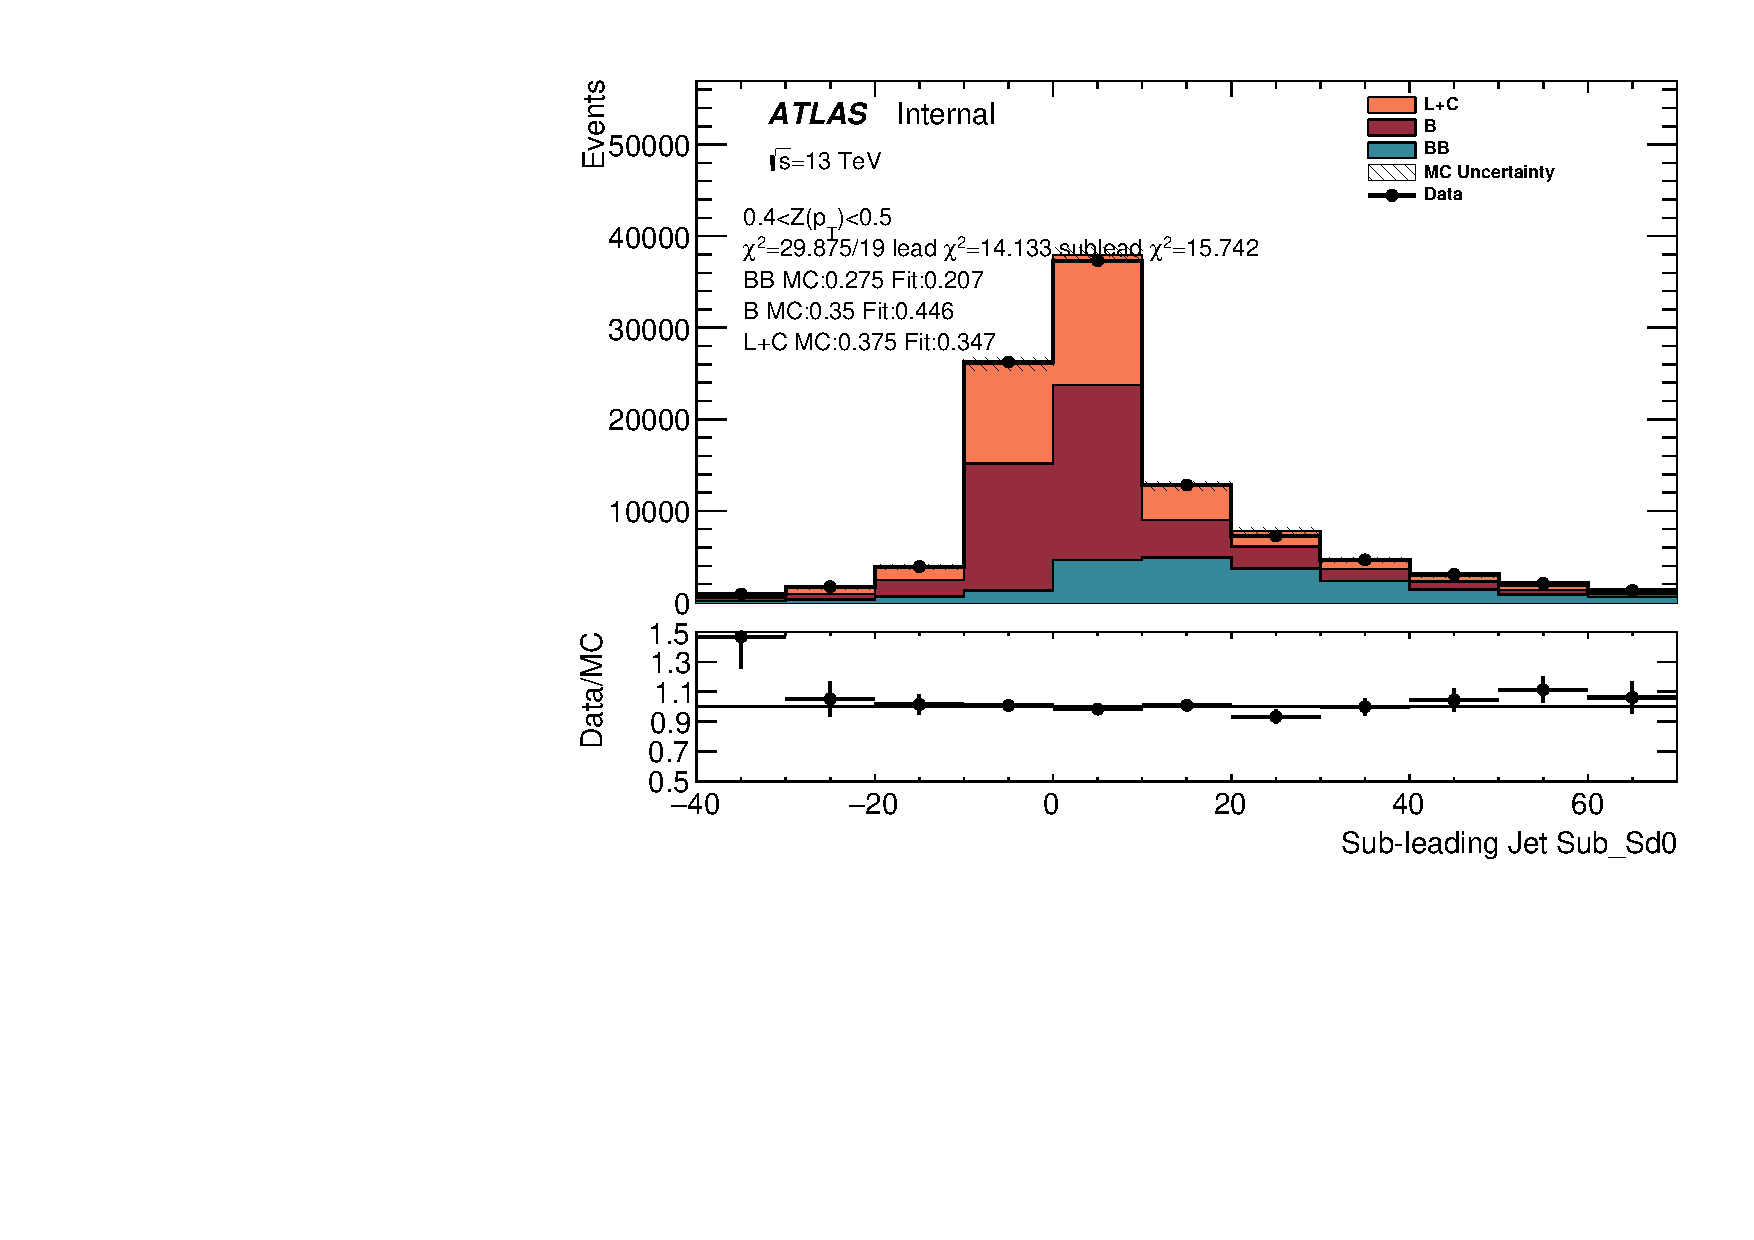
\includegraphics[width=0.32\textwidth]{figures/gbb/Sub_Sd0_Fits/Canv_Fit_04-Zp_T-05_LpT_INF_SpT_INF_coarse_y.pdf}

\caption{Post-fit \subsdzero distributions of the sub-leading track jet in bins of \zpt. }
  \label{fig:ZpT-postfits-subleading}
\end{figure}


\begin{figure}[htbp]
  \centering
 \includegraphics[width=0.45\textwidth]{figures/gbb/Sub_Sd0_Fits/Canv_ZpT_FitFrac_Original.pdf}
 \includegraphics[width=0.45\textwidth]{figures/gbb/Sub_Sd0_Fits/Canv_ZpT_FitFrac_Corrected.pdf}

\caption{MC predicted (left) and fitted (right) flavor fraction in bins of \zpt. The error bar is the quadrature sum of the uncertainty derived from fit range systematics and fit statistics as defined in Sec.~\ref{sec:gbb-sub_systematics}}
  \label{fig:ZpT-fitfrac}
\end{figure}

\begin{figure}[htbp]
  \centering
 \includegraphics[width=0.45\textwidth]{figures/gbb/Sub_Sd0_Fits/Canv_ZpT_leadCrossCheck.pdf}
 \includegraphics[width=0.45\textwidth]{figures/gbb/Sub_Sd0_Fits/Canv_ZpT_subsubCrossCheck.pdf}\\
 \includegraphics[width=0.45\textwidth]{figures/gbb/Sub_Sd0_Fits/Canv_ZpT_ptbinCrossCheck.pdf}
 \includegraphics[width=0.45\textwidth]{figures/gbb/Sub_Sd0_Fits/Canv_ZpT_noreweightCrossCheck.pdf}\\
\caption{Comparison of flavor fractions fitted (1) using \subsdzero and \sdzero (top left), (2) using \subsdzero and \subsubsdzero (top right), (3) using inclusive and $p_T$ parameterized templates (bottom left) and (4) with and without track jet kinematic reweighting (bottom right) in bins of \zpt}
  \label{fig:ZpT-fitfrac-crosscheck}
\end{figure}


\clearpage
\begin{table}[htbp]
\centering
\caption{Fit systematics size in percentage in bins of \zpt}
\label{tab:ZpTsys}
\resizebox{\textwidth}{!}{
\begin{tabular}{lrrrrr}
\hline
Syst Name     & $0<\zpt<0.1$ & $0.1<\zpt<0.2$ & $0.2<\zpt<0.3$ & $0.3<\zpt<0.4$ & $0.4<\zpt<0.5$ \\ \hline
Trk\_Eff                           & 9.08             & 1.33               & -2.55              & -4.41              & 3.95               \\
Trk\_Fake                          & 7.48             & -3.42              & 0.06               & -2.51              & 9.52               \\
Trk\_In\_Jet                       & 4.46             & -1.55              & -1.01              & -1.65              & 4.5                \\
Trk\_Sagitta                       & 6.46             & -3.28              & -6.76              & -4.85              & 0.75               \\
Trk\_d0Smear                       & 14.66            & -0.28              & -2.39              & -1.03              & 1.16               \\
FitRange\_Left                     & 0.04             & -0.39              & 1.42               & -0.93              & -0.34              \\
FitRange\_Right                    & 2.27             & -1.32              & -1.72              & -1.51              & -1.63              \\
BLUp                               & 6.1              & 2.91               & 1.88               & 1.38               & 1.99               \\
BLDn                               & -11.06           & -5.31              & -3.0               & -2.31              & -3.53              \\
BCUp                               & -11.46           & -5.39              & -3.2               & -2.65              & -3.26              \\
BCDn                               & 6.25             & 2.96               & 1.6                & 1.29               & 1.95               \\
LLUp                               & 4.69             & 3.89               & 3.04               & 1.98               & 1.44               \\
LLDn                               & -3.53            & -2.42              & -1.87              & -1.14              & -0.36              \\
LCUp                               & -2.55            & -1.04              & -0.59              & -1.54              & -0.56              \\
LCDn                               & 0.83             & 0.58               & 0.17               & 0.63               & 0.35               \\
LBUp                               & -2.06            & -1.69              & -1.05              & -1.39              & -2.23              \\
LBDn                               & 0.83             & 0.91               & 0.16               & 0.23               & 1.25               \\
CLUp                               & 5.7              & 5.29               & 3.87               & 4.85               & 5.72               \\
CLDn                               & -4.34            & -4.24              & -3.17              & -5.0               & -4.82              \\
CCUp                               & -6.61            & -6.25              & -4.69              & -4.82              & -2.19              \\
CCDn                               & 4.07             & 4.16               & 3.23               & 3.36               & 1.89               \\
CBUp                               & -1.97            & -1.92              & -1.46              & -1.58              & -2.52              \\
CBDn                               & 0.8              & 0.76               & 0.67               & 0.28               & 1.41               \\
StatUp                             & 7.11             & 4.23               & 4.03               & 3.85               & 5.23               \\
StatDn                             & -6.95            & -4.32              & -4.5               & -4.75              & -5.27              \\
FT\_EFF\_Eigen\_B\_0\_\_1down      & 0.13             & 0.15               & -0.32              & -0.25              & -0.13              \\
FT\_EFF\_Eigen\_B\_1\_\_1down      & 0.3              & 0.05               & 0.28               & -0.3               & -0.02              \\
FT\_EFF\_Eigen\_C\_0\_\_1down      & 0.08             & -0.02              & -0.38              & -0.09              & 0.26               \\
FT\_EFF\_Eigen\_C\_1\_\_1down      & -0.58            & -0.34              & -0.74              & -0.37              & 0.3                \\
FT\_EFF\_Eigen\_C\_2\_\_1down      & -0.57            & -0.38              & -0.45              & -0.75              & -0.01              \\
FT\_EFF\_Eigen\_Light\_0\_\_1down  & 1.12             & 1.0                & 1.03               & -0.17              & -0.87              \\
FT\_EFF\_Eigen\_Light\_1\_\_1down  & 1.03             & 0.68               & 0.58               & -0.41              & -0.45              \\
FT\_EFF\_Eigen\_Light\_2\_\_1down  & 0.68             & -0.91              & -0.63              & -0.32              & 0.05               \\
FT\_EFF\_Eigen\_Light\_3\_\_1down  & -0.25            & 0.0                & -0.29              & -0.23              & -0.06              \\
FT\_EFF\_extrapolation\_\_1down    & 0.8              & 0.6                & 0.42               & -0.26              & 0.12               \\
FT\_EFF\_Eigen\_B\_0\_\_1up        & -0.24            & 0.48               & -0.31              & -0.08              & 0.1                \\
FT\_EFF\_Eigen\_B\_1\_\_1up        & 0.02             & -0.11              & -0.42              & -0.39              & -0.08              \\
FT\_EFF\_Eigen\_C\_0\_\_1up        & -0.24            & 0.36               & 0.18               & -0.16              & -0.13              \\
FT\_EFF\_Eigen\_C\_1\_\_1up        & 0.36             & 0.71               & 0.84               & 0.09               & -0.19              \\
FT\_EFF\_Eigen\_C\_2\_\_1up        & 0.41             & 0.35               & 0.18               & -0.09              & -0.15              \\
FT\_EFF\_Eigen\_Light\_0\_\_1up    & -1.32            & -0.76              & -1.1               & 0.44               & 1.27               \\
FT\_EFF\_Eigen\_Light\_1\_\_1up    & -1.22            & -0.46              & -0.66              & -0.01              & 0.8                \\
FT\_EFF\_Eigen\_Light\_2\_\_1up    & 0.23             & 1.03               & 0.46               & 0.13               & 0.12               \\
FT\_EFF\_Eigen\_Light\_3\_\_1up    & 0.33             & -0.04              & 0.04               & -0.53              & 0.05               \\
FT\_EFF\_extrapolation\_\_1up      & -0.73            & -0.74              & -0.75              & -0.38              & -0.12              \\
JET\_JER                           & 4.43             & -4.16              & -1.91              & -5.57              & 5.26               \\
JET\_Comb\_Baseline\_All\_\_1up    & 13.03            & 0.75               & 3.29               & -0.58              & 4.8                \\
JET\_Comb\_Modelling\_All\_\_1down & -9.04            & -11.67             & -10.95             & -13.82             & 2.95               \\
JET\_Comb\_Modelling\_All\_\_1up   & 32.83            & 10.02              & 4.84               & -1.52              & 7.22               \\
JET\_Comb\_TotalStat\_All\_\_1down & 2.99             & 2.72               & 0.53               & -1.4               & 2.12               \\
JET\_Comb\_TotalStat\_All\_\_1up   & 1.01             & -1.4               & 0.81               & 1.37               & 1.71               \\
JET\_Comb\_Tracking\_All\_\_1down  & 4.9              & -6.24              & -1.41              & -4.93              & 10.36              \\
JET\_Comb\_Tracking\_All\_\_1up    & 12.53            & 3.18               & -2.41              & -4.71              & 3.48               \\
JET\_Comb\_Baseline\_All\_\_1down  & -4.57            & -4.51              & -2.03              & -6.83              & 3.93               \\
Sherpa                             & 39.38            & 13.9               & 7.35               & -12.26             & -7.23              \\
\end{tabular}}
\end{table}



\clearpage
\subsection{\mpt}

In total, there are five bins of the \mpt observable we are measuring. The flavor fraction fits are performed for \mpt $\in\{[-3, -2.2], [-2.2, -1.9], [-1.9, -1.5], [-1.5, -1.1], [-1.1,0]\}$. The pre-fit and post-fit Data/MC comparison are shown in Figures.~\ref{fig:fracmasspt-prefits-leading},\ref{fig:fracmasspt-prefits-subleading},\ref{fig:fracmasspt-postfits-leading},\ref{fig:fracmasspt-postfits-subleading}. The MC predicted and fitted fraction of each flavor component is shown in Fig.~\ref{fig:fracmasspt-fitfrac}. Four sets of fit cross check are performed: (1) using \sdzero as discriminant (2) using \subsubsdzero (3) using $p_T$ parameterized templates and (4) without track jet kinematics reweighting. The cross check results are summarized in Fig.~\ref{fig:fracmasspt-fitfrac-crosscheck}. We observe closure of fitted signal (`BB') event fraction in all the cross checks within fitting uncertainties. The size of each of the systematic uncertainties is summarized in Table~\ref{tab:fracmassptsys}.


\begin{figure}[htbp]
  \centering
 \includegraphics[width=0.32\textwidth]{figures/gbb/Sub_Sd0_Fits/Canv_PreFit_-3-logM_bb_over_p_TG--22_LpT_INF_SpT_INF_coarse_x.pdf}
 \includegraphics[width=0.32\textwidth]{figures/gbb/Sub_Sd0_Fits/Canv_PreFit_-22-logM_bb_over_p_TG--19_LpT_INF_SpT_INF_coarse_x.pdf}
 \includegraphics[width=0.32\textwidth]{figures/gbb/Sub_Sd0_Fits/Canv_PreFit_-19-logM_bb_over_p_TG--15_LpT_INF_SpT_INF_coarse_x.pdf}\\
 \includegraphics[width=0.32\textwidth]{figures/gbb/Sub_Sd0_Fits/Canv_PreFit_-15-logM_bb_over_p_TG--11_LpT_INF_SpT_INF_coarse_x.pdf}
 \includegraphics[width=0.32\textwidth]{figures/gbb/Sub_Sd0_Fits/Canv_PreFit_-11-logM_bb_over_p_TG-0_LpT_INF_SpT_INF_coarse_x.pdf}

\caption{Pre-fit \subsdzero distributions of the leading track jet in bins of \mpt. }
  \label{fig:fracmasspt-prefits-leading}
\end{figure}


\begin{figure}[htbp]
  \centering
 \includegraphics[width=0.32\textwidth]{figures/gbb/Sub_Sd0_Fits/Canv_PreFit_-3-logM_bb_over_p_TG--22_LpT_INF_SpT_INF_coarse_y.pdf}
 \includegraphics[width=0.32\textwidth]{figures/gbb/Sub_Sd0_Fits/Canv_PreFit_-22-logM_bb_over_p_TG--19_LpT_INF_SpT_INF_coarse_y.pdf}
 \includegraphics[width=0.32\textwidth]{figures/gbb/Sub_Sd0_Fits/Canv_PreFit_-19-logM_bb_over_p_TG--15_LpT_INF_SpT_INF_coarse_y.pdf}\\
 \includegraphics[width=0.32\textwidth]{figures/gbb/Sub_Sd0_Fits/Canv_PreFit_-15-logM_bb_over_p_TG--11_LpT_INF_SpT_INF_coarse_y.pdf}
 \includegraphics[width=0.32\textwidth]{figures/gbb/Sub_Sd0_Fits/Canv_PreFit_-11-logM_bb_over_p_TG-0_LpT_INF_SpT_INF_coarse_y.pdf}

\caption{Pre-fit \subsdzero distributions of the sub-leading track jet in bins of \mpt. }
  \label{fig:fracmasspt-prefits-subleading}
\end{figure}

\begin{figure}[htbp]
  \centering
 \includegraphics[width=0.32\textwidth]{figures/gbb/Sub_Sd0_Fits/Canv_Fit_-3-logM_bb_over_p_TG--22_LpT_INF_SpT_INF_coarse_x.pdf}
 \includegraphics[width=0.32\textwidth]{figures/gbb/Sub_Sd0_Fits/Canv_Fit_-22-logM_bb_over_p_TG--19_LpT_INF_SpT_INF_coarse_x.pdf}
 \includegraphics[width=0.32\textwidth]{figures/gbb/Sub_Sd0_Fits/Canv_Fit_-19-logM_bb_over_p_TG--15_LpT_INF_SpT_INF_coarse_x.pdf}\\
 \includegraphics[width=0.32\textwidth]{figures/gbb/Sub_Sd0_Fits/Canv_Fit_-15-logM_bb_over_p_TG--11_LpT_INF_SpT_INF_coarse_x.pdf}
 \includegraphics[width=0.32\textwidth]{figures/gbb/Sub_Sd0_Fits/Canv_Fit_-11-logM_bb_over_p_TG-0_LpT_INF_SpT_INF_coarse_x.pdf}


\caption{Post-fit \subsdzero distributions of the leading track jet in bins of \mpt. }
  \label{fig:fracmasspt-postfits-leading}
\end{figure}


\begin{figure}[htbp]
  \centering
 \includegraphics[width=0.32\textwidth]{figures/gbb/Sub_Sd0_Fits/Canv_Fit_-3-logM_bb_over_p_TG--22_LpT_INF_SpT_INF_coarse_y.pdf}
 \includegraphics[width=0.32\textwidth]{figures/gbb/Sub_Sd0_Fits/Canv_Fit_-22-logM_bb_over_p_TG--19_LpT_INF_SpT_INF_coarse_y.pdf}
 \includegraphics[width=0.32\textwidth]{figures/gbb/Sub_Sd0_Fits/Canv_Fit_-19-logM_bb_over_p_TG--15_LpT_INF_SpT_INF_coarse_y.pdf}\\
 \includegraphics[width=0.32\textwidth]{figures/gbb/Sub_Sd0_Fits/Canv_Fit_-15-logM_bb_over_p_TG--11_LpT_INF_SpT_INF_coarse_y.pdf}
 \includegraphics[width=0.32\textwidth]{figures/gbb/Sub_Sd0_Fits/Canv_Fit_-11-logM_bb_over_p_TG-0_LpT_INF_SpT_INF_coarse_y.pdf}

\caption{Post-fit \subsdzero distributions of the sub-leading track jet in bins of \mpt. }
  \label{fig:fracmasspt-postfits-subleading}
\end{figure}


\begin{figure}[htbp]
  \centering
 \includegraphics[width=0.45\textwidth]{figures/gbb/Sub_Sd0_Fits/Canv_fracmasspt_FitFrac_Original.pdf}
 \includegraphics[width=0.45\textwidth]{figures/gbb/Sub_Sd0_Fits/Canv_fracmasspt_FitFrac_Corrected.pdf}

\caption{MC predicted (left) and fitted (right) flavor fraction in bins of \mpt. The error bar is the quadrature sum of the uncertainty derived from fit range systematic uncertainties and fit statistics as defined in Sec.~\ref{sec:gbb-sub_systematics}}
  \label{fig:fracmasspt-fitfrac}
\end{figure}


\begin{figure}[htbp]
  \centering
 \includegraphics[width=0.45\textwidth]{figures/gbb/Sub_Sd0_Fits/Canv_fracmasspt_leadCrossCheck.pdf}
 \includegraphics[width=0.45\textwidth]{figures/gbb/Sub_Sd0_Fits/Canv_fracmasspt_subsubCrossCheck.pdf}\\
 \includegraphics[width=0.45\textwidth]{figures/gbb/Sub_Sd0_Fits/Canv_fracmasspt_ptbinCrossCheck.pdf}
 \includegraphics[width=0.45\textwidth]{figures/gbb/Sub_Sd0_Fits/Canv_fracmasspt_noreweightCrossCheck.pdf}\\
\caption{Comparison of flavor fractions fitted (1) using \subsdzero and \sdzero (top left), (2) using \subsdzero and \subsubsdzero (top right), (3) using inclusive and $p_T$ parameterized templates (bottom left) and (4) with and without track jet kinematic reweighting (bottom right) in bins of \mpt}
  \label{fig:fracmasspt-fitfrac-crosscheck}
\end{figure}


\clearpage
\begin{table}[htbp]
\centering
\caption{Fit systematics size in percentage in bins of \mpt}
\label{tab:fracmassptsys}
\resizebox{\textwidth}{!}{
\begin{tabular}{lrrrrr}
\hline
Syst Name     & $-3<\mpt<-2.2$ & $-2.2<\mpt<-1.9$ & $-1.9<\mpt<-1.5$ & $-1.5<\mpt<-1.1$ & $-1.1<\mpt<0$ \\ \hline
Trk\_Eff                                              & -1.03             & 2.31   & 3.04  & 1.36  & 1.1    \\
Trk\_Fake                                             & 1.83              & 1.09   & 2.01  & 2.46  & 7.22   \\
Trk\_In\_Jet                                          & -0.74             & 1.39   & -0.11 & 6.84  & -0.83  \\
Trk\_Sagitta                                          & 2.18              & -4.4   & 0.87  & -3.71 & 3.05   \\
Trk\_d0Smear                                          & 3.34              & -2.83  & 1.3   & 7.01  & 4.74   \\
FitRange\_Left                                        & -1.04             & -0.25  & 0.06  & 1.39  & 2.67   \\
FitRange\_Right                                       & 2.08              & 1.23   & -1.01 & -1.67 & -0.38  \\
BLUp                                                  & 3.79              & 1.85   & 1.9   & 2.92  & 2.39   \\
BLDn                                                  & -4.82             & -3.5   & -3.95 & -4.14 & -3.94  \\
BCUp                                                  & -4.87             & -3.53  & -3.86 & -4.07 & -3.05  \\
BCDn                                                  & 3.53              & 1.86   & 2.11  & 2.45  & 2.44   \\
LLUp                                                  & 4.53              & 2.66   & 2.99  & 3.52  & 1.93   \\
LLDn                                                  & -2.61             & -1.57  & -2.24 & -1.33 & -0.69  \\
LCUp                                                  & -0.7              & -0.51  & -0.66 & -0.52 & -1.04  \\
LCDn                                                  & 1.07              & 0.23   & 0.08  & 0.71  & 0.9    \\
LBUp                                                  & -1.0              & -1.08  & -1.29 & -1.29 & -1.45  \\
LBDn                                                  & 1.18              & 0.38   & 0.34  & 1.12  & 1.24   \\
CLUp                                                  & 5.71              & 3.96   & 4.5   & 5.73  & 5.7    \\
CLDn                                                  & -3.24             & -3.09  & -4.17 & -5.0  & -3.98  \\
CCUp                                                  & -6.98             & -4.58  & -5.51 & -5.37 & -3.22  \\
CCDn                                                  & 4.82              & 3.05   & 3.43  & 4.46  & 2.66   \\
CBUp                                                  & -0.71             & -1.2   & -1.76 & -1.7  & -2.2   \\
CBDn                                                  & 1.01              & 0.79   & 0.66  & 1.15  & 0.97   \\
StatUp                                                & 5.96              & 3.34   & 2.84  & 4.83  & 8.74   \\
StatDn                                                & -5.01             & -3.41  & -3.24 & -4.49 & -8.71  \\
FT\_EFF\_Eigen\_B\_0\_\_1down                         & 0.24              & 0.04   & -0.19 & 0.13  & -0.07  \\
FT\_EFF\_Eigen\_B\_1\_\_1down                         & -0.04             & -0.21  & -0.24 & 0.32  & 0.03   \\
FT\_EFF\_Eigen\_C\_0\_\_1down                         & -0.11             & -0.17  & -0.4  & 0.06  & 0.1    \\
FT\_EFF\_Eigen\_C\_1\_\_1down                         & -0.16             & -0.12  & -0.5  & -0.28 & 0.03   \\
FT\_EFF\_Eigen\_C\_2\_\_1down                         & 0.3               & -0.16  & -0.25 & 0.16  & -0.6   \\
FT\_EFF\_Eigen\_Light\_0\_\_1down                     & 2.26              & 1.01   & 1.0   & 1.07  & 0.15   \\
FT\_EFF\_Eigen\_Light\_1\_\_1down                     & 1.53              & 0.87   & 0.64  & 0.9   & 0.09   \\
FT\_EFF\_Eigen\_Light\_2\_\_1down                     & 1.46              & 0.45   & 0.26  & 0.57  & -0.28  \\
FT\_EFF\_Eigen\_Light\_3\_\_1down                     & 0.18              & 0.02   & -0.4  & 0.22  & -0.11  \\
FT\_EFF\_extrapolation\_\_1down                       & 0.3               & -0.37  & -0.37 & 0.29  & 0.76   \\
FT\_EFF\_Eigen\_B\_0\_\_1up                           & 0.39              & -0.25  & -0.21 & 0.38  & 0.4    \\
FT\_EFF\_Eigen\_B\_1\_\_1up                           & 0.42              & 0.09   & -0.29 & 0.26  & -0.24  \\
FT\_EFF\_Eigen\_C\_0\_\_1up                           & 0.79              & 0.05   & -0.02 & 0.59  & 0.09   \\
FT\_EFF\_Eigen\_C\_1\_\_1up                           & 1.3               & 0.24   & 0.43  & 0.81  & 0.01   \\
FT\_EFF\_Eigen\_C\_2\_\_1up                           & 0.82              & 0.03   & 0.03  & 0.47  & 0.44   \\
FT\_EFF\_Eigen\_Light\_0\_\_1up                       & -2.53             & -1.25  & -1.65 & -0.53 & 0.83   \\
FT\_EFF\_Eigen\_Light\_1\_\_1up                       & -1.55             & -0.81  & -1.28 & -0.2  & -0.32  \\
FT\_EFF\_Eigen\_Light\_2\_\_1up                       & -1.12             & -0.69  & -0.82 & -0.01 & -0.16  \\
FT\_EFF\_Eigen\_Light\_3\_\_1up                       & 0.28              & 0.04   & -0.18 & 0.1   & -0.02  \\
FT\_EFF\_extrapolation\_\_1up                         & 0.38              & -0.05  & 0.06  & 0.17  & -0.02  \\
JET\_JER                                              & -2.45             & -0.65  & 0.15  & -0.23 & 5.96   \\
JET\_Comb\_Baseline\_All\_\_1up                       & 1.37              & 3.25   & 5.41  & 3.27  & 7.06   \\
JET\_Comb\_Modelling\_All\_\_1down                    & -6.28             & -13.14 & -6.25 & -7.24 & -2.16  \\
JET\_Comb\_Modelling\_All\_\_1up                      & 13.99             & 7.81   & 7.36  & 11.62 & 13.61  \\
JET\_Comb\_TotalStat\_All\_\_1down                    & -2.1              & 1.64   & 1.96  & 3.95  & 4.36   \\
JET\_Comb\_TotalStat\_All\_\_1up                      & -1.55             & -2.57  & 3.05  & 4.59  & 5.2    \\
JET\_Comb\_Tracking\_All\_\_1down                     & -4.12             & -1.54  & 4.0   & -0.34 & 6.26   \\
JET\_Comb\_Tracking\_All\_\_1up                       & 7.82              & 3.19   & 2.13  & 2.84  & 0.71   \\
JET\_Comb\_Baseline\_All\_\_1down                     & -6.8              & -2.95  & -1.25 & -2.06 & 0.79   \\
Sherpa                                                & 10.66             & 7.09   & -1.28 & 4.09  & -10.54 \\
\end{tabular}}
\end{table}


\clearpage
\subsection{\dphi}

In total, there are five bins of the \dphi observable we are measuring. The flavor fraction fits are performed for \dphi $\in\{[0, \pi/5], [\pi/5, 2\pi/5], [2\pi/5, 3\pi/5], [3\pi/5, 4\pi/5], [4\pi/5, \pi]\}$. The pre-fit and post-fit Data/MC comparison are shown in Figures.~\ref{fig:dphi-prefits-leading},\ref{fig:dphi-prefits-subleading},\ref{fig:dphi-postfits-leading},\ref{fig:dphi-postfits-subleading}. The MC predicted and fitted fraction of each flavor component is shown in Fig.~\ref{fig:dphi-fitfrac}. Four sets of fit cross check are performed: (1) using \sdzero as discriminant (2) using \subsubsdzero (3) using $p_T$ parameterized templates and (4) without track jet kinematic reweighting. The cross check results are summarized in Fig.~\ref{fig:dphi-fitfrac-crosscheck}. We observe closure of fitted signal (`BB') event fraction in all the cross checks within fitting uncertainties. The size of each of the systematic uncertainties is summarized in Table.\ref{tab:dphisys}.


\begin{figure}[htbp]
  \centering
 \includegraphics[width=0.32\textwidth]{figures/gbb/Sub_Sd0_Fits/Canv_PreFit_0-Deltaphi-0628_LpT_INF_SpT_INF_coarse_x.pdf}
 \includegraphics[width=0.32\textwidth]{figures/gbb/Sub_Sd0_Fits/Canv_PreFit_0628-Deltaphi-1256_LpT_INF_SpT_INF_coarse_x.pdf}
 \includegraphics[width=0.32\textwidth]{figures/gbb/Sub_Sd0_Fits/Canv_PreFit_1256-Deltaphi-1884_LpT_INF_SpT_INF_coarse_x.pdf}\\
 \includegraphics[width=0.32\textwidth]{figures/gbb/Sub_Sd0_Fits/Canv_PreFit_1884-Deltaphi-2512_LpT_INF_SpT_INF_coarse_x.pdf}
 \includegraphics[width=0.32\textwidth]{figures/gbb/Sub_Sd0_Fits/Canv_PreFit_2512-Deltaphi-3140_LpT_INF_SpT_INF_coarse_x.pdf}

\caption{Pre-fit \subsdzero distributions of the leading track jet in bins of \dphi. }
  \label{fig:dphi-prefits-leading}
\end{figure}


\begin{figure}[htbp]
  \centering
 \includegraphics[width=0.32\textwidth]{figures/gbb/Sub_Sd0_Fits/Canv_PreFit_0-Deltaphi-0628_LpT_INF_SpT_INF_coarse_y.pdf}
 \includegraphics[width=0.32\textwidth]{figures/gbb/Sub_Sd0_Fits/Canv_PreFit_0628-Deltaphi-1256_LpT_INF_SpT_INF_coarse_y.pdf}
 \includegraphics[width=0.32\textwidth]{figures/gbb/Sub_Sd0_Fits/Canv_PreFit_1256-Deltaphi-1884_LpT_INF_SpT_INF_coarse_y.pdf}\\
 \includegraphics[width=0.32\textwidth]{figures/gbb/Sub_Sd0_Fits/Canv_PreFit_1884-Deltaphi-2512_LpT_INF_SpT_INF_coarse_y.pdf}
 \includegraphics[width=0.32\textwidth]{figures/gbb/Sub_Sd0_Fits/Canv_PreFit_2512-Deltaphi-3140_LpT_INF_SpT_INF_coarse_y.pdf}

\caption{Pre-fit \subsdzero distributions of the sub-leading track jet in bins of \dphi. }
  \label{fig:dphi-prefits-subleading}
\end{figure}

\begin{figure}[htbp]
  \centering
 \includegraphics[width=0.32\textwidth]{figures/gbb/Sub_Sd0_Fits/Canv_Fit_0-Deltaphi-0628_LpT_INF_SpT_INF_coarse_x.pdf}
 \includegraphics[width=0.32\textwidth]{figures/gbb/Sub_Sd0_Fits/Canv_Fit_0628-Deltaphi-1256_LpT_INF_SpT_INF_coarse_x.pdf}
 \includegraphics[width=0.32\textwidth]{figures/gbb/Sub_Sd0_Fits/Canv_Fit_1256-Deltaphi-1884_LpT_INF_SpT_INF_coarse_x.pdf}\\
 \includegraphics[width=0.32\textwidth]{figures/gbb/Sub_Sd0_Fits/Canv_Fit_1884-Deltaphi-2512_LpT_INF_SpT_INF_coarse_x.pdf}
 \includegraphics[width=0.32\textwidth]{figures/gbb/Sub_Sd0_Fits/Canv_Fit_2512-Deltaphi-3140_LpT_INF_SpT_INF_coarse_x.pdf}


\caption{Post-fit \subsdzero distributions of the leading track jet in bins of \dphi. }
  \label{fig:dphi-postfits-leading}
\end{figure}


\begin{figure}[htbp]
  \centering
 \includegraphics[width=0.32\textwidth]{figures/gbb/Sub_Sd0_Fits/Canv_Fit_0-Deltaphi-0628_LpT_INF_SpT_INF_coarse_y.pdf}
 \includegraphics[width=0.32\textwidth]{figures/gbb/Sub_Sd0_Fits/Canv_Fit_0628-Deltaphi-1256_LpT_INF_SpT_INF_coarse_y.pdf}
 \includegraphics[width=0.32\textwidth]{figures/gbb/Sub_Sd0_Fits/Canv_Fit_1256-Deltaphi-1884_LpT_INF_SpT_INF_coarse_y.pdf}\\
 \includegraphics[width=0.32\textwidth]{figures/gbb/Sub_Sd0_Fits/Canv_Fit_1884-Deltaphi-2512_LpT_INF_SpT_INF_coarse_y.pdf}
 \includegraphics[width=0.32\textwidth]{figures/gbb/Sub_Sd0_Fits/Canv_Fit_2512-Deltaphi-3140_LpT_INF_SpT_INF_coarse_y.pdf}

\caption{Post-fit \subsdzero distributions of the sub-leading track jet in bins of \dphi. }
  \label{fig:dphi-postfits-subleading}
\end{figure}


\begin{figure}[htbp]
  \centering
 \includegraphics[width=0.45\textwidth]{figures/gbb/Sub_Sd0_Fits/Canv_dphi_FitFrac_Original.pdf}
 \includegraphics[width=0.45\textwidth]{figures/gbb/Sub_Sd0_Fits/Canv_dphi_FitFrac_Corrected.pdf}
\caption{MC Predicted (left) and fitted (right) flavor fraction in bins of \dphi. The error bar is the quadrature sum of the uncertainty derived from fit range systematics and fit statistics as defined in Sec.~\ref{sec:gbb-sub_systematics}}
  \label{fig:dphi-fitfrac}
\end{figure}


\begin{figure}[htbp]
  \centering
 \includegraphics[width=0.45\textwidth]{figures/gbb/Sub_Sd0_Fits/Canv_dphi_leadCrossCheck.pdf}
 \includegraphics[width=0.45\textwidth]{figures/gbb/Sub_Sd0_Fits/Canv_dphi_subsubCrossCheck.pdf}\\
 \includegraphics[width=0.45\textwidth]{figures/gbb/Sub_Sd0_Fits/Canv_dphi_ptbinCrossCheck.pdf}
 \includegraphics[width=0.45\textwidth]{figures/gbb/Sub_Sd0_Fits/Canv_dphi_noreweightCrossCheck.pdf}\\
\caption{Comparison of flavor fractions fitted (1) using \subsdzero and \sdzero (top left), (2) using \subsdzero and \subsubsdzero (top right), (3) using inclusive and $p_T$ parameterized templates (bottom left) and (4) with and without track jet kinematic reweighting (bottom right) in bins of \dphi}
  \label{fig:dphi-fitfrac-crosscheck}
\end{figure}


\clearpage
\begin{table}[htbp]
\centering
\caption{Fit systematics size in percentage in bins of \dphi}
\label{tab:dphisys}
\resizebox{\textwidth}{!}{
\begin{tabular}{lrrrrr}
\hline
Syst Name                          & 0$<\Delta\phi<$0.6 & 0.6$<\Delta\phi<$1.2 & 1.2$<\Delta\phi<$1.8 & 1.8$<\Delta\phi<$2.4 & 2.4$<\Delta\phi<$3.2 \\ \hline
Trk\_Eff                           & 0.46               & 8.58                 & 2.6                  & 5.63                 & -0.67                \\
Trk\_Fake                          & -1.28              & 3.84                 & 9.64                 & 5.93                 & 3.64                 \\
Trk\_In\_Jet                       & -0.67              & 5.78                 & 9.2                  & 5.98                 & -2.07                \\
Trk\_Sagitta                       & -1.73              & 3.2                  & 2.64                 & 1.08                 & -1.95                \\
Trk\_d0Smear                       & -0.9               & 8.5                  & 3.19                 & 8.35                 & -3.76                \\
FitRange\_Left                     & 0.35               & 1.02                 & -0.18                & 0.16                 & -0.06                \\
FitRange\_Right                    & 1.0                & 0.19                 & -0.55                & -1.84                & -0.29                \\
BLUp                               & 2.42               & 1.93                 & 2.8                  & 2.74                 & 1.65                 \\
BLDn                               & -4.01              & -2.81                & -4.87                & -4.89                & -2.78                \\
BCUp                               & -3.82              & -2.94                & -4.76                & -4.75                & -2.75                \\
BCDn                               & 2.39               & 2.0                  & 2.67                 & 2.87                 & 1.56                 \\
LLUp                               & 3.96               & 3.49                 & 4.31                 & 4.71                 & 3.05                 \\
LLDn                               & -2.57              & -1.77                & -2.92                & -3.05                & -1.81                \\
LCUp                               & -0.88              & -0.49                & -0.99                & -0.94                & -0.14                \\
LCDn                               & 0.83               & 0.8                  & 0.66                 & 0.65                 & 0.26                 \\
LBUp                               & -1.26              & -0.94                & -1.06                & -1.64                & -1.27                \\
LBDn                               & 0.97               & 0.63                 & 0.51                 & 0.78                 & 0.51                 \\
CLUp                               & 4.46               & 4.85                 & 3.11                 & 3.99                 & 3.67                 \\
CLDn                               & -3.5               & -4.28                & -2.53                & -3.29                & -2.87                \\
CCUp                               & -4.99              & -5.77                & -4.81                & -6.23                & -4.69                \\
CCDn                               & 3.43               & 4.22                 & 3.35                 & 4.28                 & 3.33                 \\
CBUp                               & -2.16              & -1.24                & -1.61                & -1.26                & -1.54                \\
CBDn                               & 0.98               & 1.03                 & 0.55                 & 0.52                 & 0.77                 \\
StatUp                             & 4.0                & 4.83                 & 4.49                 & 4.44                 & 4.3                  \\
StatDn                             & -4.2               & -4.63                & -4.29                & -4.51                & -3.87                \\
FT\_EFF\_Eigen\_B\_0\_\_1down      & 0.17               & 0.26                 & 0.07                 & 0.22                 & 0.1                  \\
FT\_EFF\_Eigen\_B\_1\_\_1down      & -0.16              & 0.07                 & -0.21                & -0.04                & -0.21                \\
FT\_EFF\_Eigen\_C\_0\_\_1down      & -0.29              & -0.13                & -0.41                & -0.35                & -0.04                \\
FT\_EFF\_Eigen\_C\_1\_\_1down      & -0.42              & -0.22                & -0.71                & -0.73                & -0.54                \\
FT\_EFF\_Eigen\_C\_2\_\_1down      & -0.35              & 0.09                 & -0.5                 & -0.57                & 0.13                 \\
FT\_EFF\_Eigen\_Light\_0\_\_1down  & 1.97               & 1.68                 & 1.93                 & 2.23                 & 1.74                 \\
FT\_EFF\_Eigen\_Light\_1\_\_1down  & 1.54               & 1.15                 & 1.66                 & 1.87                 & 1.25                 \\
FT\_EFF\_Eigen\_Light\_2\_\_1down  & 1.86               & 1.68                 & 1.21                 & 1.4                  & 1.33                 \\
FT\_EFF\_Eigen\_Light\_3\_\_1down  & -0.12              & 0.36                 & -0.02                & -0.18                & 0.07                 \\
FT\_EFF\_extrapolation\_\_1down    & -0.93              & -0.92                & -0.62                & -0.43                & -0.71                \\
FT\_EFF\_Eigen\_B\_0\_\_1up        & 0.06               & 0.3                  & 0.18                 & -0.17                & 0.03                 \\
FT\_EFF\_Eigen\_B\_1\_\_1up        & 0.35               & 0.28                 & 0.22                 & 0.16                 & 0.1                  \\
FT\_EFF\_Eigen\_C\_0\_\_1up        & 0.39               & 0.17                 & 0.3                  & 0.57                 & 0.29                 \\
FT\_EFF\_Eigen\_C\_1\_\_1up        & 1.02               & 0.44                 & 1.0                  & 1.05                 & 0.69                 \\
FT\_EFF\_Eigen\_C\_2\_\_1up        & 0.27               & 0.26                 & 0.39                 & 0.55                 & 0.39                 \\
FT\_EFF\_Eigen\_Light\_0\_\_1up    & -2.39              & -1.81                & -2.45                & -3.63                & -1.78                \\
FT\_EFF\_Eigen\_Light\_1\_\_1up    & -1.56              & -0.93                & -1.77                & -2.25                & -1.38                \\
FT\_EFF\_Eigen\_Light\_2\_\_1up    & -2.06              & -1.82                & -1.21                & -1.46                & -1.29                \\
FT\_EFF\_Eigen\_Light\_3\_\_1up    & -0.01              & -0.11                & -0.12                & 0.48                 & -0.06                \\
FT\_EFF\_extrapolation\_\_1up      & 1.02               & 0.78                 & 0.39                 & 0.25                 & 0.77                 \\
JET\_JER                           & 0.05               & 6.45                 & 3.34                 & 2.48                 & -1.94                \\
JET\_Comb\_Baseline\_All\_\_1up    & 3.31               & 12.12                & 7.8                  & 13.27                & 2.89                 \\
JET\_Comb\_Modelling\_All\_\_1down & -10.82             & -11.16               & -11.74               & -3.48                & -15.9                \\
JET\_Comb\_Modelling\_All\_\_1up   & 12.41              & 19.56                & 19.19                & 15.06                & 6.25                 \\
JET\_Comb\_TotalStat\_All\_\_1down & 0.81               & 7.21                 & 5.52                 & 5.06                 & -0.65                \\
JET\_Comb\_TotalStat\_All\_\_1up   & -2.85              & 3.38                 & 8.91                 & 6.43                 & 1.02                 \\
JET\_Comb\_Tracking\_All\_\_1down  & -1.57              & 5.69                 & 3.94                 & 3.76                 & -0.9                 \\
JET\_Comb\_Tracking\_All\_\_1up    & 3.8                & 6.89                 & 6.85                 & 9.34                 & -4.82                \\
JET\_Comb\_Baseline\_All\_\_1down  & -2.15              & -1.04                & -4.0                 & -1.58                & -7.59                \\
Sherpa                             & -9.44              & 7.11                 & 18.0                 & -16.63               & 7.05                 \\
\end{tabular}}
\end{table}

\clearpage

